
\documentclass[12pt]{iopart}
\pdfoutput=1
\usepackage{iopams}
\usepackage{amssymb, epsfig}
%\usepackage{amsmath, amssymb,epsfig}
\usepackage{latexsym}

%\usepackage[hypertex,hyperindex]{hyperref}
%\usepackage{showkeys}
\usepackage{graphicx}
\usepackage{color}

\newcommand{\pf}{\mbox{pf}}

\begin{document}
	
	\bibliographystyle{plain}
	\def\debproof{\noindent {\bf Proof.} }
	\def\finproof{\hfill {\small $\Box$} \\}
	%\renewcommand{\theequation}{\arabic{section}.\arabic{equation}}
	
	\makeatletter % `@' now normal "letter"
	\@addtoreset{equation}{section}
	\makeatother  % `@' is restored as "non-letter"
	\renewcommand\theequation{{\thesection}.{\arabic{equation}}}
	\title[]{}
	
	
	
	\maketitle
	\newcommand{\eps}{\varepsilon}
	\newcommand{\RR}{\mathcal{R}}
	\newtheorem{lem}{Lemma}[section]
	\newtheorem{prop}{Proposition}[section]
	\newtheorem{cor}{Corollary}[section]
	\newtheorem{thm}{Theorem}[section]
	\newtheorem{rem}{Remark}[section]
	\newtheorem{alg}{Algorithm}[section]
	\newtheorem{assum}{Assumption}[section]
	\newtheorem{definition}{Definition}[section]
	
	
	\newcounter{RomanNumber}
	\newcommand{\MyRoman}[1]{\rm\setcounter{RomanNumber}{#1}\Roman{RomanNumber}}
	
	\newcommand{\bL}{\mathbf{L}}
	\newcommand{\bH}{\mathbf{H}}
	\newcommand{\bW}{\mathbf{W}}
	\newcommand{\bP}{\mathbf{P}}
	\newcommand{\bQ}{\mathbf{Q}}
	\newcommand{\bp}{\mathbf{p}}
	\newcommand{\bq}{\mathbf{q}}
	\newcommand{\uL}{u_{_{\rm L}}}
	\newcommand{\vL}{v_{_{\rm L}}}
	\newcommand{\tuL}{\tilde u_{_{\rm L}}}
	\newcommand{\tvL}{\tilde v_{_{\rm L}}}
	\newcommand{\fL}{f_{_{\rm L}}}
	\newcommand{\gL}{g_{_{\rm L}}}
	\newcommand{\bpL}{\bp_{_{\rm L}}}
	\newcommand{\bqL}{\bq_{_{\rm L}}}
	\newcommand{\tbpL}{\tilde{\bp}_{_{\rm L}}}
	\newcommand{\tbqL}{\tilde{\bq}_{_{\rm L}}}
	\newcommand{\tbpLf}{\tilde{\bp}_{_{\rm L,1}}}
	\newcommand{\tbpLs}{\tilde{\bp}_{_{\rm L,2}}}
	\newcommand{\tbqLf}{\tilde{\bq}_{_{\rm L,1}}}
	\newcommand{\tbqLs}{\tilde{\bq}_{_{\rm L,2}}}
	\newcommand{\bn}{\nu}
	\newcommand{\bv}{\mathbf{v}}
	\newcommand{\om}{\omega}
	\newcommand{\pa}{\partial}
	\newcommand{\la}{\langle}
	\newcommand{\ra}{\rangle}
	\newcommand{\lla}{\la{\hskip -2pt}\la}
	\newcommand{\rra}{\ra{\hskip -2pt}\ra}
	\newcommand{\jj}{\|{\hskip -0.8pt} |}
	\newcommand{\al}{\alpha}
	\newcommand{\ze}{\zeta}
	\newcommand{\si}{\sigma}
	\newcommand{\ep}{\varepsilon}
	\newcommand{\na}{\nabla}
	\newcommand{\vp}{\varphi}
	\newcommand{\ga}{\gamma}
	\newcommand{\Ga}{\Gamma}
	\newcommand{\Om}{\Omega}
	\newcommand{\de}{\delta}
	\newcommand{\Th}{\Theta}
	\newcommand{\De}{\Delta}
	\newcommand{\Lam}{\Lambda}
	\newcommand{\lam}{\lambda}
	\newcommand{\tri}{\triangle}
	\newcommand{\lj}{[{\hskip -2pt} [}
	\newcommand{\rj}{]{\hskip -2pt} ]}
	\newcommand{\bks}{\backslash}
	%\newcommand{\diag}{\mathrm{diag}}
	\newcommand{\diam}{\mathrm{diam}}
	\newcommand{\osc}{\mathrm{osc}}
	\newcommand{\meas}{\mathrm{meas}}
	\newcommand{\dist}{\mathrm{dist}}
	
	\newcommand{\mL}{\mathscr{L}}
	\newcommand{\cT}{{\cal T}}
	\newcommand{\cM}{{\cal M}}
	\newcommand{\cE}{{\cal E}}
	\newcommand{\cL}{{\cal L}}
	\newcommand{\cF}{{\cal F}}
	\newcommand{\cB}{{\cal B}}
	\newcommand{\PML}{{\rm PML}}
	\newcommand{\FEM}{{\rm FEM}}
	\newcommand{\rd}{\,\mathrm{d}}
	
	\renewcommand{\i}{\mathbf{i}}
	\renewcommand{\v}{\mathbf{v}}
	\renewcommand{\u}{\mathbf{u}}
	\renewcommand{\r}{\mathbf{r}}
	\newcommand{\R}{{\mathbb{R}}}
	\newcommand{\Z}{{\mathbb{Z}}}
	\newcommand{\C}{{\mathbb{C}}}
	\renewcommand{\Re}{\mathrm{Re}\,}
	\renewcommand{\Im}{\mathrm{Im}\,}
	\renewcommand{\div}{\mathrm{div}}
	\newcommand{\curl}{\mathrm{curl}}
	\newcommand{\Curl}{\mathbf{curl}}
	
	
	%%%%%%%%%%%%%%%%%%%%%%%%%%%%%%%%%%%%%%%%%%%%%%%%%%%%%%%%%%%%%%%%%%%%
	\newcommand{\be}{\begin{eqnarray}}
	\newcommand{\ee}{\end{eqnarray}}
	\newcommand{\ben}{\begin{eqnarray*}}
		\newcommand{\een}{\end{eqnarray*}}
	\newcommand{\nn}{\nonumber}
	
	
	\section{Estimate of Dirichlet Green Tensor}
	We need the following slight generalization of Van der Corput lemma for the oscillatory integral \cite[P.152]{grafakos}.
	\begin{lem}\label{van}
		Let $-\infty<a<b<\infty$, and $u$ is a $C^k$ function $u$ in $(a,b)$. \\
		1. If $|u'(t)|\ge 1$ for $t\in (a,b)$ and $u'$ is monotone in (a,b), then for any $\phi(t)$ in $(a,b)$ with integrable derivatives
		\ben
		\left|\int^b_a e^{\i\lambda u(t)}\phi(t)dt\right|\le
		3\lambda^{-1}\left[|\phi(b)|+\int^b_a|\phi'(t)|dt\right].
		\een
		2. For all $k\geq2$, if $|u^{(k)}(t)|\ge 1$ for $t\in (a,b)$ , then for any $\phi(t)$ in $(a,b)$ with integrable derivatives
		\ben
		\left|\int^b_a e^{\i\lambda u(t)}\phi(t)dt\right|\le
		12k\lambda^{-1/k}\left[|\phi(b)|+\int^b_a|\phi'(t)|dt\right].
		\een
	\end{lem}
	\debproof
	The assertion can be proved by extending the Van der Corptut lemma in \cite{grafakos}. Here we omit the details.
	\finproof
	We recall following lemma, see e.g. \cite{Wong_Asymptotic}:
	\begin{lem} \label{asym_frac}
		Let $F(\rho,a)=\int_{0}^{a} t^{\alpha-1}f(t)e^{-\i\rho t}dt$ where $0<a\leq+\infty$, $0<\alpha<1$, $\rho>0$ and $t^{\alpha-1}f\in L^1(0,a)$, then we have
		\be
		|F(\rho,a)|\leq C(\frac{1}{\rho^\alpha}f(0)+\frac{1}{\rho}(a^{\alpha-1}f(a)+|t^{\alpha-1}f|_{L^1(0,a)})
		\ee
	\end{lem}
	\debproof
	Put
	\be
	g_0(t)=t^{\alpha-1}e^{-\i\rho t}
	\ee
	and define
	\be
	g_1(t)=-\int_{t}^{t-\i\infty} x^{\alpha-1}e^{-\i\rho x} dx
	\ee
	where the path of integration is the vertical line $x=t-\i y, y\geq0$. It is easy to show that $g_1(t)'=g_0(t)$. Substituting $x=t-\i y$ into $g_1(t)$, we have
	\be
	g_1(t)=\i\int_{0}^{\infty}(t-\i y)^{\alpha-1}e^{-\i\rho t}e^{-\rho y} d y
	\ee
	Upon integration by parts, we have
	\ben
	F(\rho,a)&=&\int_{0}^{a}f(t)dg_1(t)\\
	&=&e^{-\i\frac{\alpha\pi}{2}}f(0)\Gamma(\alpha)\frac{1}{\rho^{\alpha}}+f(a)g_1(a)-\int_{0}^{a}f'(t)g_1(t)dt \\
	&=&e^{-\i\frac{\alpha\pi}{2}}f(0)\Gamma(\alpha)\frac{1}{\rho^{\alpha}} -\i
	\int_{0}^{\infty}e^{-\rho y}dy \int_{0}^{a}f'(t)(t-\i y)^{\alpha-1}e^{-\i\rho t}dt
	\een
	Let 
	\ben
	h(y)=\int_{0}^{a}f'(t)(t-\i y)^{\alpha-1}e^{-\i\rho t}dt
	\een
	and observe that
	\ben
	|h(y)|\leq\int_{0}^{a}|f'(t)|(t^2+y^2)^{\frac{\alpha-1}{2}}dt
	\een
	\finproof
	\begin{lem} \label{asym_frac_2}
		Let $F(\rho,a)=\int_{0}^{a} t^{-1/2}f(t)e^{-\i\rho t}dt$ where $0<a\leq+\infty$ and $\rho>0$, then we have
		\be
		& &|F(\rho,a)-e^{-\i\frac{\pi}{4}}f(0)\Gamma(1/2)\frac{1}{\rho^{1/2}}|\\
		&\leq& C (\int_{0}^{\infty}e^{-\rho y}dy \int_{0}^{a}|f'(t)|(t^2+y^2)^{-\frac{1}{4}}dt+\frac{1}{\rho}a^{-1/2}f(a))
		\ee
	\end{lem}
	\debproof
	Put
	\be
	g_0(t)=t^{-1/2}e^{-\i\rho t}
	\ee
	and define
	\be
	g_1(t)=-\int_{t}^{t-\i\infty} x^{-1/2}e^{-\i\rho x} dx
	\ee
	where the path of integration is the vertical line $x=t-\i y, y\geq0$. It is easy to show that $g_1‘(t)=g_0(t)$. Substituting $x=t-\i y$ into $g_1(t)$, we have
	\be
	g_1(t)=\i\int_{0}^{\infty}(t-\i y)^{-1/2}e^{-\i\rho t}e^{-\rho y} d y
	\ee
	Upon integration by parts, we have
	\ben
	F(\rho,a)&=&\int_{0}^{a}f(t)dg_1(t)\\
	&=&e^{-\i\frac{\pi}{4}}f(0)\Gamma(1/2)\frac{1}{\rho^{1/2}}+f(a)g_1(a)-\int_{0}^{a}f'(t)g_1(t)dt \\
	&=&e^{-\i\frac{\pi}{4}}f(0)\Gamma(1/2)\frac{1}{\rho^{1/2}}+\i f(a)\int_{0}^{\infty}(a-\i y)^{-1/2}e^{-\i\rho t}e^{-\rho y} d y
	\\ & & -\i
	\int_{0}^{\infty}e^{-\rho y}dy \int_{0}^{a}f'(t)(t-\i y)^{-1/2}e^{-\i\rho t}dt
	\een
	Let 
	\ben
	h(y)=\int_{0}^{a}f'(t)(t-\i y)^{-1/2}e^{-\i\rho t}dt
	\een
	and observe that
	\ben
	|h(y)|\leq\int_{0}^{a}|f'(t)|(t^2+y^2)^{-\frac{1}{4}}dt
	\een
	It is easy to see that
	\ben
	|g_1(a)|\leq a^{-1/2}\int_{0}^{\infty} e^{-\rho y}dy\leq C\frac{1}{\rho}
	\een
	\finproof
	\begin{lem}
		Assume that $0<\kappa:=\sin\phi_\kappa<1,0<\phi_\kappa<\pi/2$, $0\leq\phi\leq\pi/2$ and $-\pi/2<t_1<t_2<\pi/2$ satisfy that $\kappa^2=\sin^2(\phi+t_1)=\sin^2(\phi+t_2)$. Let $f(\theta)$:
		\be
		f(t,\phi):=F(\sin(t+\phi),\cos(t+\phi),(\kappa^2-\sin^2(t+\phi))^{1/2})
		\ee
		be a function in $C^\infty(([-\pi/2,\pi/2]\bks\{t_1,t_2\})\times[0,\pi/2])$. Moreover, there exits $\epsilon>0$ such that $f(\theta)$ can be represented as
		\be\label{convention_1}
		f(t,\phi)=g_1(t,\phi)+g_2(t,\phi)(\kappa^2-\sin^2(t+\phi))^{1/2})^{N/2}
		\ee 
		where $g_1,g_2\in C^\infty((\bigcup\limits_{i=1,2}(t_i-\epsilon,t_i+\epsilon))\times[0,\pi/2]))$ and $N=\pm1$. Then for any $\rho\geq1$, we have
		\be\nn
		\bigg|I(\rho,\phi):=\int_{-\pi/2}^{\pi/2}f(\theta)e^{\i\rho\cos\theta}d\theta
		-\frac{N+1}{2}\bigg(\frac{2\pi}{\rho}\bigg)^{1/2}f(0) e^{\i\rho-\i\pi/4}\bigg| \\
		\leq C\frac{1}{\rho^{(2+N)/4}}
		\ee	
	\end{lem}
	\debproof
	The proof will be split into two parts about whether $\phi$ equal to $\phi_\kappa$. 
	
	If $\phi\neq\phi_\kappa$,  there exists $0<\delta<\pi/4$ such that
	\be \label{assume_1}
	|(\kappa^2-\sin^2(t+\phi))^{1/2}|>\frac{1}{2}|(\kappa^2-\sin^2\phi)^{1/2}|
	\ee
	for any $t\in(-\delta,\delta)$. Let $\chi_\delta\in C^\infty_0(-\pi/2,\pi/2)$ be the cut-off function with that $0\leq\chi_\delta\leq1$, $\chi_\delta=1$ in $(-\delta/2,\delta/2)$ and $\chi_\delta=0$  in $(-\pi/2,\pi/2)\bks(-\delta,\delta)$. Then we can divide $I$ into two parts such that
	\ben\label{I_splits}
	I=\int_{-\delta}^{\delta} f(t) \chi_\delta(t)e^{\i \rho\cos t} dt +
	\int_{-\pi/2}^{\pi/2} f(t) (1-\chi_\delta(t))e^{\i \rho\cos t} dt  \\ 
	=: I_{1} + I_{2}
	\een
	Subtitating $t(s)=2\arcsin s/2$ for t in $I_{1}$, we can obtain
	\be
	I_{1}&=&\int_\R f(t(s))\chi_\delta(t(s))\frac{1}{\sqrt{1-s^2/4}}e^{\i  \rho}e^{-\i \rho s^2/2} ds \\
	&=&\int_\R h_\delta(s)e^{\i \rho}e^{-\i \rho s^2/2} ds
	\ee
	It is easy to see that $h_\delta(s)\in C^4_0(\R)$. By the lemma of the stationary phase for quadratic term in \cite{Evans2010}, we have
	\be
	I_{1}=e^{\i  \rho}\int_\R h_\delta(s)e^{-\i\frac{\rho}{2}s^2}ds=
	e^{\i  \rho}\int_\R \widehat{h_\delta}(y)\alpha(-y)dy
	\ee
	where
	\be
	\alpha(y)=(\frac{1}{2\pi  \rho})^{1/2}e^{-\i\pi/4}e^{\frac{\i}{2  \rho}y^2} \\
	=(\frac{1}{2\pi  \rho})^{1/2}e^{-\i\pi/4}(1+O(\frac{y^2}{\rho}))
	\ee
	Consequently
	\be
	I_{1}=(\frac{1}{2\pi  \rho})^{1/2}e^{\i  \rho-\i\pi/4}
	\int_\R \widehat{h_\delta}(y)(1+\frac{1}{ \rho}O(y^2)) dy
	\ee
	Moreover, $\int_\R \widehat{h_\delta}(y)dy=2\pi h_\delta(0)$ and $|\int_\R \widehat{h_\delta}(y)y^2 dy|<C$ since $\widehat{h_\delta}(y)=O(1/y^4)$. Now, it turns to estimate $I_{2}$. 
	
	When $N=1$, using integration by parts, we have
	\be
	|I_{2}|&=&\Bigg|\int_{(-\frac{\pi}{2},\frac{\pi}{2})\bks(-\frac{\delta}{2},\frac{\delta}{2})}f(t) (1-\chi_\delta(t))/\sin t \ \  de^{\i \rho\cos t} \Bigg| \\
	\\
	&\leq& C\frac{1}{\rho}+\Bigg|\int_{(-\frac{\pi}{2},\frac{\pi}{2})\bks(-\frac{\delta}{2},\frac{\delta}{2})}(f(t) (1-\chi_\delta(t))/\sin t)' \ e^{\i \rho\cos t} dt\Bigg| \\
	&\leq& C\frac{1}{\rho}
	\ee
	From above analysis, we obtain
	\be
	\bigg|I(\rho,\phi)
	-\bigg(\frac{2\pi}{\rho}\bigg)^{1/2}f(0) e^{\i\rho-\i\pi/4}\bigg| 
	\leq C(\phi)\frac{1}{\rho}
	\ee
	When $N=-1$, we can not use integration by parts again since $f'(\theta)$ is not integrable. However,  for any $0<\lambda_1<1$ and $1<\lambda_2<1/\kappa$, there exists $0<\sigma<\epsilon$, such that $\chi:=((t_1-\sigma,t_1+\sigma)\cup(t_2-\sigma,t_2+\sigma))\cap(-\delta,\delta)=0$, dependent on $\lambda_1,\lambda_2$ and
	\be \label{assume2}
	\lambda_1\kappa<|\sin (t+\phi)|<\lambda_2\kappa.
	\ee
	for any $t\in\chi$. 
	
	We only analysis the integral on $\chi_{1}=(t_1-\sigma,t_1+\sigma)\cap[-\pi/2,\pi/2]$ here, which denoted by $I_{\chi_1}$, the proof of $I_{\chi_2}$ is similar. It is easy to see that $\sin (t+\phi)$ is monotonic in $\chi_1$. Without loss of generality, we assume that $\sin (t_1-\sigma+\phi)<\kappa<\sin (t_1+\sigma+\phi)$. Let $\sin (t+\phi) = \kappa \sin \theta$ and the implicit mapping from $\theta$ to $t$ is denoted by $t(\theta)$ while the inverse mapping by $\theta(t)$, taking the interval $\chi_1$ onto $L_\theta : \theta_1\rightarrow\pi/2\rightarrow\pi/2-\i\theta_2$ where $\sin(t_1-\sigma+\phi)=\kappa\sin \theta_1,\sin(t_1+\sigma+\phi)=\kappa\sin(\pi/2-\i\theta_2)$. By substituting $t(\theta)$ into $I_{\chi_1}$, we have
	\be
	I_{\chi_1}&=&\int_{t_1-\sigma}^{t_1+\sigma}\frac{f(t)(\kappa^2-\sin^2(t+\phi))^{1/2}}{(\kappa^2-\sin^2(t+\phi))^{1/2}} e^{\i\rho\cos t}\\
	&=&\int_{L_\theta}\frac{\kappa f(t(\theta))\cos\theta}{(1-\kappa^2\sin^2\theta)^{1/2}}e^{\i
		\rho(\cos(t(\theta)))} d\theta \\
	&=&\int_{L_\theta}\frac{\kappa g_1(t(\theta))\cos\theta+g_2(t(\theta))}{(1-\kappa^2\sin^2\theta)^{1/2}}e^{\i
		\rho(\cos(t(\theta)))} d\theta \\
	&:=&\int_{L_\theta}\frac{h(\theta)}{(1-\kappa^2\sin^2\theta)^{1/2}}e^{\i
		\rho(\cos(t(\theta)))} d\theta 
	\ee
	Observe that $h(\theta)$ and $\pa h/\pa\theta$ are integrable on the path $L_\theta$ by (\ref{convention_1}). A simple computation show that
	\ben\hspace{-0.5cm}
	\frac{dt(\theta)}{d\theta}=\frac{\kappa\cos\theta}{\cos(t+\phi)} \ \ \ \ \ \
	\frac{d^2 t(\theta)}{dt^2}=\frac{\kappa^2\cos^2\theta\sin(t+\phi)-\kappa\sin\theta\cos^2(t+\phi)}{\cos^3(t+\phi)}
	\een
	Then we can obtain
	\ben
	\frac{d\cos t}{d\theta}&=&\frac{-\kappa\sin t\cos\theta}{\cos(t+\phi)} \\
	\frac{d^2\cos t}{d\theta^2}&=&\frac{d^2\cos t}{dt^2}(\frac{dt}{d\theta})^2+\frac{d\cos t}{dt}\frac{d^2t}{d\theta^2} \\
	&=&\frac{-\kappa^2\cos^2\theta\cos t}{\cos^2(t+\phi)}+\frac{\kappa\sin\theta\cos^2(t+\phi)\sin t -\kappa^2\cos^2\theta\sin(t+\phi)\sin t}{\cos^3(t+\phi)} \\
	&=&\frac{-\kappa^2\cos^2\theta\cos\phi+\kappa\sin\theta\cos^2(t+\phi)\sin t}{\cos^3(t+\phi)} \\
	&=&\frac{(\sin^2(t+\phi)-\kappa^2)\cos\phi+\cos^2(t+\phi)\sin(t+\phi)\sin t}{\cos^3(t+\phi)}
	\een
	Since $|\sin t|>|\sin\delta|$ and $1-\lambda_2^2\kappa^2<\cos^2(t+\phi)<1-\lambda_1^2\kappa^2$ for $t\in\chi_1$, it follows that $\theta=\pi/2$ is the only stationary point of $\cos(t(\theta))$ and 
	\be
	\Bigg|\frac{d^2\cos t}{d\theta^2}(\pi/2)\Bigg|=\frac{(1-\kappa^2)\kappa}{(1-\kappa^2)^{3/2}}|\sin t|>\frac{(1-\kappa^2)\kappa}{(1-\kappa^2)^{3/2}}\sin \delta
	\ee
	Therefore, we can choose appropriate $\lambda_1,\lambda_2$ such that 
	\be
	|\frac{d^2\cos t}{d\theta^2}|>\frac{(1-\kappa^2)\kappa}{(1-\kappa^2)^{3/2}}\sin \delta
	\ee
	for any 
	$\theta\in \theta(\chi_1)$. According to lemma (\ref{van}), we obtian $|I_{\chi_1}|\leq C\frac{1}{\rho^{1/2}}$, and also $|I_{\chi_2}|\leq C\frac{1}{\rho^{1/2}}$. Using integration by parts, we get
	\ben
	\Bigg|\int_{[-\pi/2,\pi/2]\bks((-\delta,\delta)\cup\chi)}f(t) (1-\chi_\delta(t)) e^{\i \rho\cos t} dt\Bigg| 
	\leq C\frac{1}{\rho}
	\een
	Consequently, for $N=-1$ and $\phi\neq\phi_\kappa$, we get $|I(\rho,\phi)|\leq\frac{1}{\rho^{1/2}}$.
	
	We now turn to the case of $\phi=\phi_\kappa$. By (\ref{convention_1}), we can define $\chi_\epsilon$ similarly and also decompose $I$ into $I_1$ and $I_2$. Using the same agurement above, we can easily carry out that:
	for $N=1$, we have $|I_2|\leq C \frac{1}{\rho}$;
	for $N=-1$, we have $|I_2|\leq C \frac{1}{\rho^{1/2}}$. Finally, it remains to analysis $I_1$. By (\ref{convention_1}), we have
	\ben\hspace{-2cm}
	I_1&=&\int_{-\epsilon}^{\epsilon}g_1\chi_\epsilon+g_2\chi_\epsilon(\sin^2\phi_{\kappa}-\sin^2(t+\phi_\kappa))^{N/2}e^{\i\rho\cos t}dt \\ \hspace{-2cm}
	&=&\int_{-\epsilon}^{\epsilon}g_1\chi_\epsilon+g_2\chi_\epsilon(-2(\sin\phi_{\kappa}+\sin(t+\phi_\kappa))\cos\frac{2\phi_\kappa+t}{2}\sin t/2)^{N/2}e^{\i\rho\cos t}dt \\ \hspace{-2cm}
	&=&\int_\R g_1\chi_\epsilon+g_2\chi_\epsilon((\sin\phi_{\kappa}+\sin(t+\phi_\kappa))\cos\frac{2\phi_\kappa+t}{2})^{N/2}(-2\sin t/2)^{N/2}e^{\i\rho\cos t}dt
	\een
	Also, subtituting $t(s)=2\arcsin s/2$ for t in $I_{1}$, it follows that
	\be
	I_1&=&\int_\R h_1(s) e^{-\i\rho\frac{s^2}{2}}+h_2(s)(-s)^{N/2} e^{-\i\rho\frac{s^2}{2}}\\
	&=&I_{11}+I_{12}
	\ee
	where 
	\ben\hspace{-1cm}
	h_1(s)=g_1(t(s))\chi_\epsilon(t(s))\sqrt{1-s^2/4}  \ e^{\i\rho} \\\hspace{-1cm}
	h_2(s)=g_2\chi_\epsilon((\sin\phi_{\kappa}+\sin(t+\phi_\kappa))\cos\frac{2\phi_\kappa+t}{2})^{N/2}_{t=t(s)}\sqrt{1-s^2/4} \ e^{\i\rho}
	\een
	and $h_1(s),h_2(s)\in C^\infty_c(\R)$. Using stationary phase lemma similarly, if $N=1$, 
	\be
	I_{11}&=&\bigg(\frac{2\pi}{\rho}\bigg)^{1/2}g_1(0) e^{\i\rho-\i\pi/4}+O(\frac{1}{\rho})\\
	&=&\bigg(\frac{2\pi}{\rho}\bigg)^{1/2}f(0) e^{\i\rho-\i\pi/4}+O(\frac{1}{\rho})
	\ee
	if $N=-1$, we get $|I_{11}|\leq C\frac{1}{\rho^{1/2}}$.
	For $I_{12}$, we have
	\be
	I_{12}&=&\int_{0}^{\infty}(\i h_2(s)+h_2(-s)) s^{N/2}\ e^{-\i\rho s^2/2} ds \\ 
	&=&\frac{1}{2}\int_{0}^{\infty} (\i h_2(\sqrt{s})+h_2(-\sqrt{s})) s^{N/4-1/2} e^{-\i\rho s/2} ds
	\ee
	By lemma (\ref{asym_frac}), we get $|I_{12}|\leq C\frac{1}{\rho^{(N+2)/4}}$.
	\finproof
	\section{Some draft about Green Tensor Analysis}
	Let substitute $\xi=k\sin\theta$ into integral and shift the variable, we have
	\be
	I(y)=\int_\R f(\xi)e^{\i \xi y_1+\mu(\xi) y_2} d\xi =\int_\R f(\xi)e^{\i \xi (y_1-z_1)+\mu(\xi) (y_2-z_2)}e^{\i \xi z_1 +\mu(\xi) z_2} d\xi \\
	=k\int_{L} f(k\sin\theta)\cos\theta e^{\i k|y-z|\cos(\theta-\eta)}e^{\i|z|\cos(\theta-\phi)} d\theta\\
	=k\int_{L_\phi} f(k\sin(\theta+\phi))\cos(\theta+\phi) e^{\i k|y-z|\cos(\theta+\phi-\eta)}e^{\i|z|\cos\theta} d\theta\\
	=k\int_{L} f(k\sin(\theta+\phi))\cos(\theta+\phi) e^{\i k|y-z|\cos(\theta+\phi-\eta)}e^{\i|z|\cos\theta} d\theta
	\ee
	where $y_1,y_2>0,\sin\phi=\frac{z_1}{|z|},\cos\phi=\frac{z_2}{|z|},0<\phi<\pi/2$ and $\sin\eta=\frac{y_1-z_1}{|y-z|},\cos\eta=\frac{y_2-z_2}{|y-z|},0<\eta<\pi$. It is easy to see that $\phi+\eta<\pi$. Roughly, using stationary phase lemma, we obtain:
	\be
	I(y)=f(k\sin\phi)k\cos\phi e^{\i k|y-z|\cos(\phi-\eta)}(\frac{2\pi}{|z|})^{1/2}e^{\i|z|-\i\frac{\pi}{4}}(1+O(\frac{1}{|z|}))
	\ee
	\be
	\cos(a+\i b)=\frac{e^b+e^{-b}}{2}\cos a+\i\frac{e^{-b}-e^b}{2}\sin a \\
	\sin(a+\i b)=\frac{e^b+e^{-b}}{2}\sin a+\i\frac{e^{b}-e^{-b}}{2}\cos a
	\ee
	When $\theta\in(-a-\pi/2,-a-\pi/2+\i\infty)$, let $\theta=-a-\pi/2\i t$, where $t>0,0\leq
	a\leq\phi$, then
	\be\nn
	-\Im(|z|\cos\theta+|y-z|\cos(\theta+\phi-\eta))\\
	=|z|\sin(a+\pi/2)+|y-z|\sin(a+\pi/2-\phi+\eta) \\
	=|z|\cos a+|y-z|\cos(a-\phi+\eta) \\
	=|z|\cos a +\cos a|y-z|(\cos\phi\cos\eta+\sin\phi\sin\eta)\\
	+\sin a |y-z|(\sin\phi\cos\eta-\cos\phi\sin\eta)\\
	=|z|\cos a +\cos a((y_2-z_2)\cos\phi+(y_1-z_1)\sin\phi)\\
	+\sin a((y_2-z_2)\sin\phi-(y_1-z_1)\cos\phi) \\
	=y_1\sin(\phi-a)+y_2\cos(\phi-a)>0
	\ee
	Now, Using Cauchy Integral Theorem, we have
	\be
	I(y)=k\int_{L} f(k\sin(\theta+\phi))\cos(\theta+\phi) e^{\i k|y-z|\cos(\theta+\phi-\eta)}e^{\i|z|\cos\theta} d\theta
	\ee
	Let $L_1=(-\pi/2,-\pi/2+\i\infty)$ and $\theta=-\pi/2+\i t,t>0$, then
	\be
	I_1(y)=k\int_{L_1} f(k\sin(\theta+\phi))\cos(\theta+\phi) e^{\i k|y-z|\cos(\theta+\phi-\eta)}e^{\i|z|\cos\theta} d\theta \\
	=
	\ee
	\be
	I(y)=f(k\sin\phi)k\cos\phi e^{\i k|y-z|\cos(\phi-\eta)}(\frac{2\pi}{|z|})^{1/2}e^{\i|z|-\i\frac{\pi}{4}}\\
	+\frac{kz_2}{|z|}O(\Bigg(\frac{1}{k|z|}\Bigg)^{3/4}+\frac{1}{k|y|})+\frac{kz_1}{|z|}O(\Bigg(\frac{1}{k|z|}\Bigg)^{5/4}+\Bigg(\frac{1}{k|y|}\Bigg)^2)
	\ee
	It is easy to see
	\be
	\int_{-d}^{d}\frac{k}{(k|x-z|)^\alpha}\frac{1}{(k|x-y|)^\beta} dx_1\leq C(\frac{1}{(kz_2)^{\alpha+\beta-1}}+\frac{1}{(ky_2)^{\alpha+\beta-1}})
	\ee
	where $z,y\in\R^2_+$, $x\in\Gamma_0$ and $\alpha+\beta>0$.
	\be
	e^{\i \mu  y_2+\i\xi(x_1-y_1)}=e^{\i\mu y_2 -\i y_2/\tan\phi}=e^{\i y_2(\mu-\xi/\tan\phi)}
	\ee
	Another method
	\be
	\int_{-\pi/2}^{\pi/2}f(k\sin(\theta+\psi))k\cos(\theta+\psi)e^{\i k|x-y|\cos\theta}\\
	=\int_{-\pi/2}^{\pi/2}f(k\sin(\theta+\psi))k\cos(\theta+\psi)e^{\i k|x-y|\cos(\theta+\psi-\psi)} \\
	=\int_{-\pi/2}^{\pi/2}f(k\sin(\theta+\psi))k\cos(\theta+\psi)e^{\i ky_2\cos(\theta+\psi)+\i k|x_1-y_1|\sin(\theta+\psi)} \\
	=\int_{-\pi/2}^{\pi/2}f(k\sin(\theta+\psi))k\cos(\theta+\psi)\\
	e^{\i k(y_2-z_2)\cos(\theta+\psi)+\i k(|x_1-y_1|-|x_1-z_1|)\sin(\theta+\psi)+\i k|z|\cos(\theta+\psi-\phi)}
	\ee
	\section{Finite Aperture Point Spread Function}
	If $x\in \Gamma_0$ and $z,y\in \R^2_+$, by lemma (\ref{pr_dgreen}) we have
	\be \hspace{-2.5cm} \nn
	G(x,y)=\frac{\i k_s}{\mu\sqrt{2\pi}}\frac{1}{\delta(\xi)}\Bigg(
	\begin{array}{cc}
		\mu_s\beta & \xi\beta \\
		2\xi\mu_s\mu_p & 2\xi^2\mu_p
	\end{array}\Bigg)_{\xi=k_s\frac{x_1-y_1}{|x-y|}} \frac{y_2}{|x-y|}\frac{1}{(k_s|x-y|)^{1/2}}
	e^{\i k_s|x-y|-\i\frac{\pi}{4}}\\ \hspace{-1cm}
	+\frac{\i k_p}{\mu\sqrt{2\pi}}\frac{1}{\delta(\xi)}	
	\Bigg(\begin{array}{cc}
		2\xi^2\mu_s & -2\xi\mu_s\mu_p\\
		-\xi\beta & \mu_p\beta
	\end{array} \Bigg)_{\xi=k_p\frac{x_1-y_1}{|x-y|}} \frac{y_2}{|x-y|}\frac{1}{(k_p|x-y|)^{1/2}}
	e^{\i k_p|x-y|-\i\frac{\pi}{4}} \\ \hspace{-1cm}\nn
	+O(\frac{y_2}{|x-y|}\frac{1}{(k_s|x-y|)^{3/4}}+\frac{|x_1-y_1|}{|x-y|}\frac{1}{(k_s|x-y|)^{5/4}}) \\ \hspace{-1cm}\nn
	:=\mathcal{G}_s(x,y)+\mathcal{G}_p(x,y)+O(\frac{y_2}{|x-y|}\frac{1}{(k_s|x-y|)^{3/4}}+\frac{|x_1-y_1|}{|x-y|}\frac{1}{(k_s|x-y|)^{5/4}})
	\ee
	\be
	\hspace{-2.5cm} \nn
	T_D(x,z)=\frac{k_s}{\sqrt{2\pi}}\frac{1}{\gamma(\xi)}\Bigg(
	\begin{array}{cc}
		\mu_s\mu_p & \xi\mu_p \\
		\xi\mu_s & \xi^2
	\end{array}\Bigg)_{\xi=k_s\frac{x_1-z_1}{|x-z|}} \frac{z_2}{|x-z|}\frac{1}{(k_s|x-z|)^{1/2}}
	e^{\i k_s|x-z|-\i\frac{\pi}{4}}\\ \hspace{-1cm}
	+\frac{ k_p}{\sqrt{2\pi}}\frac{1}{\gamma(\xi)}	
	\Bigg(\begin{array}{cc}
		\xi^2 & -\xi\mu_p \\
		-\xi\mu_s & \mu_p\mu_s
	\end{array} \Bigg)_{\xi=k_p\frac{x_1-z_1}{|x-z|}} \frac{z_2}{|x-z|}\frac{1}{(k_p|x-z|)^{1/2}}
	e^{\i k_p|x-z|-\i\frac{\pi}{4}}\\ \hspace{-1cm} \nn
	+O(\frac{k_s z_2}{|x-z|}\frac{1}{(k_s|x-z|)^{3/4}}+\frac{k_s|x_1-z_1|}{|x-z|}\frac{1}{(k_s|x-z|)^{5/4}}) \\ \hspace{-1cm}\nn
	:=\mathcal{T}_s(x,z)+\mathcal{T}_p(x,z)+O(\frac{k_s z_2}{|x-z|}\frac{1}{(k_s|x-z|)^{3/4}}+\frac{k_s|x_1-z_1|}{|x-z|}\frac{1}{(k_s|x-z|)^{5/4}})
	\ee
	Now we consider the finite aperture point spread function $J_d(z,y)$:
	\be
	\int_{-d}^{d} (T_D(x_1,0;z_1,z_2))^T\overline{G(x_1,0;y_1,y_2)}dx_1
	\ee
	Recall following standard asymptotic expansion:
	\be
	|x-y|=|x-z|+\widehat{x-z}\cdot (z-y)+O(\frac{|y-z|^2}{|x-z|}) \\
	|y|^{-\alpha}=|z|^{-\alpha}(1+\frac{|y|-|z|}{|z|})^{-\alpha}=|z|^{-\alpha}(1+O(\frac{|y-z|}{|z|})) \\
	e^{\i t}=1+O(t) \\
	|a^{1/2}-b^{1/2}|\leq C \sqrt{|a-b|}
	\ee
	where $x,y,z\in \R^2$, $t,a,b\in\R $ and $\alpha>0$.
	\begin{lem}
		For any $z,y\in \R^2_+$, $J_d(z,y)=F(z,y)+O((1+\frac{|y-z|}{z_2})(\frac{1}{k_s z_2})^{1/4}+\frac{(k_s|y-z|)^2}{k_s z_2}+(\frac{|y-z|}{z_2})^{1/2})$, where
		\be \hspace{-2.2cm}
		F(z,y) =-\frac{\i}{2\pi\mu}\int_{\theta^d_1}^{\theta^d_2}f_s(\theta)
		\Bigg(
		\begin{array}{cc}
			\sin^2\theta & \sin\theta\cos\theta  \\
			\sin\theta\cos\theta & \cos^2\theta
		\end{array}\Bigg)
		e^{\i k_s(z_1-y_1)\cos\theta+\i k_s(z_2-y_2)\sin\theta} d\theta \\ \hspace{-1.2cm}
		-\frac{\i}{2\pi\mu} \int_{\theta^d_1}^{\theta^d_2}f_p(\theta)
		\Bigg(
		\begin{array}{cc}
			\cos^2\theta & -\sin\theta\cos\theta  \\
			-\sin\theta\cos\theta & \sin^2\theta
		\end{array}\Bigg)
		e^{\i k_p(z_1-y_1)\cos\theta+\i k_p(z_2-y_2)\sin\theta}d\theta
		\ee
		and
		\ben\hspace{-3cm}
		f_s(\theta)=\frac{\sin\theta((\kappa^2-\cos^2\theta)^{1/2}(1-2\cos^2\theta)+2\overline{(\kappa^2-\cos^2\theta)^{1/2}}\cos^2\theta)}
		{(\cos^2\theta+\sin\theta(\kappa^2-\cos^2\theta)^{1/2})\overline{((1-2\cos^2\theta)^2+4\cos^2\theta\sin\theta(\kappa^2-\cos\theta)^{1/2}})} \\\hspace{-3cm}
		f_p(\theta)=\frac{\sin\theta(1/\kappa^2-\cos^2\theta)^{1/2}}
		{(\cos^2\theta+\sin\theta(1/\kappa^2-\cos^2\theta)^{1/2})((1/\kappa^2-2\cos^2\theta)^2+4\cos^2\theta\sin\theta(1/\kappa^2-\cos\theta)^{1/2})}
		\een
		where $0<\theta^d_1<\pi/2<\theta^d_2<\pi$ and $z_2=(d+z_1)\tan \theta^d_1=(z_1-d)\tan \theta^d_2$.
	\end{lem}
	\debproof
	\ben
	\frac{y_2}{|x-y|}\frac{1}{(k_s|x-y|)^{3/4}}+\frac{|x_1-y_1|}{|x-y|}\frac{1}{(k_s|x-y|)^{5/4}} \\ \hspace{-0.5cm}
	=(\frac{ z_2}{|x-z|}\frac{1}{(k_s|x-z|)^{3/4}}+\frac{|x_1-z_1|}{|x-z|}\frac{1}{(k_s|x-z|)^{5/4}})(1+O(\frac{|y-z|}{|x-z|}))
	\een
	\ben
	|\mu_\i(k_j\frac{x_1-y_1}{|x-y|})-\mu_\i(k_j\frac{x_1-z_1}{|x-z|})| \\  \leq
	C k_j \sqrt{\Big|\frac{x_1-y_1}{|x-y|}-\frac{x_1-z_1}{|x-z|}\Big|} \leq C k_j \Big(\frac{|y-z|}{|x-z|}\Big)^{1/2}
	\een
	where $i,j=s,p$. By above, we can obtain
	\be \label{G_sprin}\hspace{-2cm}
	\mathcal{G}_s(x,y)=\mathcal{G}_s(x,z)e^{\i k_s\widehat{x-z}\cdot (z-y)}+O(\frac{(k_s|y-z|)^2}{(k_s|x-z|)^{3/2}})+O(\frac{(k_s|y-z|)^{1/2}}{k_s|x-z|}) \\ \hspace{-2cm}\label{G_pprin}
	\mathcal{G}_p(x,y)=\mathcal{G}_p(x,z)e^{\i k_p\widehat{x-z}\cdot (z-y)}+O(\frac{(k_p|y-z|)^2}{(k_p|x-z|)^{3/2}})+O(\frac{(k_p|y-z|)^{1/2}}{k_p|x-z|})
	\ee
	For $l>1$, a simple computation show that
	\be\label{int_d} \hspace{-1cm}
	\int_{-d}^{d}\frac{k_s }{(k_s|x-z|)^l}dx_1=\frac{1}{(k_s z_2)^{l-1}}\int_{\frac{-d-z_1}{z_2}}^{\frac{d-z_1}{z_2}}\frac{1}{(1+t^2)^{l/2}} dt\leq C\frac{1}{(k_s z_2)^{l-1}}
	\ee
	Let
	\be
	\mathcal{G}_\alpha(x,y)=\frac{\i}{\sqrt{2\pi}\mu}g_\alpha(\frac{x_1-y_1}{|x-y|},\kappa)\frac{1}{(k_\alpha|x-y|)^{1/2}}e^{\i k_\alpha|x-y|-\i\frac{\pi}{4}} \\
	\mathcal{T}_\alpha(x,y)=\frac{k_\alpha}{\sqrt{2\pi}}
	t_\alpha(\frac{x_1-z_1}{|x-z|},\kappa)\frac{1}{(k_s|x-z|)^{1/2}}
	e^{\i k_\alpha|x-z|-\i\frac{\pi}{4}}
	\ee
	where $\alpha=s,p$.
	Now, by substituting (\ref{G_sprin}-\ref{G_pprin}) into $J_d(z,y)$ and using inequality (\ref{int_d}), we have
	\be\nn\hspace{-1.5cm}\nn
	J_d(z,y)=\frac{-\i}{2\pi\mu}\int_{-d}^{d}t_s(\frac{x_1-z_1}{|x-z|},\kappa)^T\overline{g_s(\frac{x_1-z_1}{|x-z|},\kappa)}\frac{e^{\i k_s\widehat{x-z}\cdot (y-z)}}{|x-z|}\\
	+t_p(\frac{x_1-z_1}{|x-z|},\kappa)^T\overline{g_p(\frac{x_1-z_1}{|x-z|},\kappa)}\frac{e^{\i k_p\widehat{x-z}\cdot (y-z)}}{|x-z|}dx_1\\
	-\frac{\i}{2\pi\mu}\int_{-d}^{d}t_p(\frac{x_1-z_1}{|x-z|},\kappa)^T\overline{g_s(\frac{x_1-z_1}{|x-z|},\kappa)}\frac{e^{\i k_s\widehat{x-z}\cdot (y-z)}}{|x-z|}\\
	+t_s(\frac{x_1-z_1}{|x-z|},\kappa)^T\overline{g_p(\frac{x_1-z_1}{|x-z|},\kappa)}\frac{e^{\i k_p\widehat{x-z}\cdot (y-z)}}{|x-z|}dx_1\\
	+O((1+\frac{|y-z|}{z_2})(\frac{1}{k_s z_2})^{1/4}+\frac{(k_s|y-z|)^2}{k_s z_2}+(\frac{|y-z|}{z_2})^{1/2})\\
	:=F(z,y)+R(z,y)\\
	+O((1+\frac{|y-z|}{z_2})(\frac{1}{k_s z_2})^{1/4}+\frac{(k_s|y-z|)^2}{k_s z_2}+(\frac{|y-z|}{z_2})^{1/2})
	\ee
	We denote $\widehat{x-z}=x-z/|x-z|=(cos(\phi+\pi),\sin(\phi+\pi))$, then taking the substitution $x_1=z_1-z_2\cot\phi$, we obtain
	\be
	F(z,y)&=&\frac{-\i}{2\pi\mu} \int_{\theta^d_1}^{\theta^d_2}A_s(\phi,\kappa)e^{\i k_s(z_1-y_1)\cos\phi+\i k_s(z_2-y_2)\sin\phi} \\
	&+&\frac{-\i}{2\pi\mu} \int_{\theta^d_1}^{\theta^d_2}A_p(\phi,\kappa)e^{\i k_p(z_1-y_1)\cos\phi+\i k_p(z_2-y_2)\sin\phi}
	\ee
	\be
	R(z,y)&=&\frac{-\i}{2\pi\mu} \int_{\theta^d_1}^{\theta^d_2}B_s(\phi,\kappa)e^{\i k_s(z_1-y_1)\cos\phi+\i k_s(z_2-y_2)\sin\phi+(k_p-k_s)|x-z|} \\
	&+&\frac{-\i}{2\pi\mu} \int_{\theta^d_1}^{\theta^d_2}B_p(\phi,\kappa)e^{\i k_p(z_1-y_1)\cos\phi+\i k_p(z_2-y_2)\sin\phi+(k_s-k_p)|x-z|}
	\ee
	It is easy to see that $|R(z,y)|\leq C\frac{|z-y|}{z_2}$.
	\finproof
	
	Let 
	\ben
	g(x_1)=\frac{1}{((x_1-z_1)^2+z_2^2)^{3/4}((x_1-y_1)^2+y_2^2)^{1/4}}\\
	\phi(x_1)=((x_1-z_1)^2+z_2^2)^{1/2}-((x_1-y_1)^2+y_2^2)^{1/2}
	\een
	Then, we have
	\ben
	g'(x_1)=-g(x_1)[\frac{3(x_1-z_1)}{2((x_1-z_1)^2+z_2^2)}+\frac{(x_1-y_1)}{2((x_1-y_1)^2+y_2^2)}]\\
	\phi'(x_1)=\frac{x_1-z_1}{((x_1-z_1)^2+z_2^2)^{1/2}}-\frac{x_1-y_1}{((x_1-y_1)^2+y_2^2)^{1/2}}\\
	=\frac{\frac{(x_1-z_1)^2}{(x_1-z_1)^2+z_2^2}-\frac{(x_1-y_1)^2}{(x_1-y_1)^2+y_2^2}}{\frac{x_1-z_1}{((x_1-z_1)^2+z_2^2)^{1/2}}+\frac{x_1-y_1}{((x_1-y_1)^2+y_2^2)^{1/2}}}\\
	=\frac{(x_1-z_1)^2y_2^2-(x_1-y_1)^2z_2^2}{(\frac{x_1-z_1}{((x_1-z_1)^2+z_2^2)^{1/2}}+\frac{x_1-y_1}{((x_1-y_1)^2+y_2^2)^{1/2}})((x_1-z_1)^2+z_2^2)((x_1-y_1)^2+y_2^2)}\\
	\phi''(x_1)=\frac{z_2^2}{((x_1-z_1)^2+z_2^2)^{3/2}}-\frac{y_2^2}{((x_1-y_1)^2+y_2^2)^{3/2}}
	\een
	Using integration by parts, we can obtain
	\ben
	\int_{-d}^{d} g(x_1)e^{\i \phi(x_1)}dx_1 \\
	=(\frac{g(d)}{\phi'(d)}e^{\i \phi(d)}-\frac{g(-d)}{\phi'(-d)}e^{\i \phi(-d)})-\int_{-d}^{d}\frac{g'(x_1)}{\phi'(x_1)}-\frac{g(x_1)\phi''(x_1)}{(\phi'(x_1))^2}dx_1
	\een
	Assume that 
	\ben
	|y_1|\leq c_0 d  \ \ \ |z_1|\leq c_0 d \ \ \ h\leq y_2,z_2\leq c_1h \ \ \ d\leq c_2
	h    
	\een
	where $0<c_0<1$. Let define $0<\theta_y,\theta_z<\pi$ such that 
	\ben
	\cos\theta_y=\frac{x_1-y_1}{((x_1-y_1)^2+y_2^2)^{1/2}} \\
	\cos\theta_z=\frac{x_1-z_1}{((x_1-z_1)^2+z_2^2)^{1/2}}
	\een
	By mean value theorem and the law of sines, we get
	\ben
	|\phi'(x_1)|&=&|\cos\theta_z-\cos\theta_y|=|\sin\theta'||\theta_z-\theta_y|\\
	&\geq&\frac{h}{(1+c_0)d}|\sin(\theta_z-\theta_y)| \\
	&=&\frac{h}{(1+c_0)d}\frac{|z-y|}{|x-y|}\sin\theta_{|x-y|}\\
	&=&\frac{h}{(1+c_0)d}\frac{|z-y|}{|x-z|}\sin\theta_{|x-z|} \\
	&\geq&\frac{h^2}{(1+c_0)^2d^2}\frac{|z-y|}{|x-y|}\\
\mbox{or}	&\geq&\frac{h^2}{(1+c_0)^2d^2}\frac{|z-y|}{|x-z|}
	\een
	Then we have
	\ben
	|\frac{g(x_1)}{\phi'(x_1)}|&\leq&\frac{(1+c_0)^2 d^2}{h^2}\frac{1}{|z-y||x-y|^{1/2}|x-z|^{1/2}} \\
	&\leq&C\frac{ d^2}{h^3}\frac{1}{|z-y|}
	\een
	Moreover, by mean value theorem agian, we have
	\ben
	|\phi''(x_1)|&=&|\frac{\sin^2\theta_z}{|x-z|}-\frac{\sin^2\theta_y}{|x-y|}|\\
	&=&|\frac{2\sin\theta'\cos\theta'}{|x-y'|}(\theta_z-\theta_y)-\frac{\sin^2\theta'}{|x-y'|^2}(|x-z|-|x-y|)| \\
	&\leq&\pi\frac{|\sin(\theta_z-\theta_y)}{h}+\frac{|z-y|}{h^2} \\
	&\leq&\pi\frac{|\sin\theta_{|x-z|}||z-y|}{h|x-z|}+\frac{|z-y|}{h^2} \\
	&\leq&C\frac{|z-y|}{h^2}
	\een
	Now, it is easy to see that
	\ben
	& &
	\Big|\int_{-d}^{d}\frac{g'(x_1)}{\phi'(x_1)}-\frac{g(x_1)\phi''(x_1)}{(\phi'(x_1))^2}dx_1\Big| \\
	&\leq&C\frac{ d^3}{h^4}\frac{1}{|z-y|}+C\frac{ d^3}{h^3}\frac{1}{|z-y|}\frac{d^2}{h^3}
	\een
	Based on the above analysis, we can obtain
	\ben
	|\int_{-d}^{d}z_2 g(x_1)e^{\i \phi(x_1)}|\leq C((\frac{d}{h})^{2}+(\frac{d}{h})^{3}+(\frac{d}{h})^{5})\frac{1}{|z-y|}
	\een
	\section{2017.11.08}
	\ben
	\sin\phi_\kappa-\sin(t+\phi)=-2\cos(\frac{\phi_\kappa+\phi+t}{2})\sin(\frac{t+\phi-\phi_\kappa}{2}) \\
	\sin(\frac{t+\phi-\phi_\kappa}{2})=\sin\frac{t}{2}\cos(\frac{\phi-\phi_\kappa}{2})+\cos\frac{t}{2}\sin(\frac{\phi-\phi_\kappa}{2})
	\een
	Some think, substituting $t=2\arcsin s/2$ into following integral
	\ben
	\int_{0}^{\infty}\chi(t)(\sin\phi_\kappa-\sin(t+\phi))^{1/2} e^{-\i\rho \cos t} \\
	=\int_{0}^{\infty}\chi(t(s))(-s\cos(\frac{\phi-\phi_\kappa}{2})-\sqrt{4-s^2}\sin(\frac{\phi-\phi_\kappa}{2})^{1/2} e^{-\i\rho s^2/2}\\
	=\int_{0}^{\infty}\chi(t)(-\sqrt{t}\cos(\frac{\phi-\phi_\kappa}{2})-\sqrt{4-t}\sin(\frac{\phi-\phi_\kappa}{2})^{1/2}t^{-1/2} e^{-\i\rho t/2}
	\een
	Let
	\ben
	f(t)= t^{-1/2} e^{-\i\rho t/2} \\
	g(t)=-\int_{t}^{t-\i\infty}x^{-1/2}e^{-\i\rho x/2} dx \\
	=\i\int_{0}^{\infty}(t-\i x)^{-1/2}e^{-\i\rho t-\rho x} dx
	\een
	It is easy to see that $g'(t)=f(t)$. Then we have
	\ben
	=\int_{0}^{\infty}\chi(t)(-\sqrt{t}\cos(\frac{\phi-\phi_\kappa}{2})-\sqrt{4-t}\sin(\frac{\phi-\phi_\kappa}{2})^{1/2}t^{-1/2} e^{-\i\rho t/2}\\
	=\chi(0)(-2\sin(\frac{\phi-\phi_\kappa}{2}))^{1/2}g(0) \\
	-\int_{0}^{\infty}(\chi(t)(-\sqrt{t}\cos(\frac{\phi-\phi_\kappa}{2})-\sqrt{4-t}\sin(\frac{\phi-\phi_\kappa}{2})^{1/2})'g(t)dt
	\een
	We get
	\ben\hspace{-2cm}
	g(x)=\int_{0}^{\infty}\chi(t)(-\sqrt{t}\cos(\frac{\phi-\phi_\kappa}{2})-\sqrt{4-t}\sin(\frac{\phi-\phi_\kappa}{2})^{-1/2}t^{-1/2}(t-\i x)^{-1/2}e^{-\i\rho t} dt \\
	R(\rho)=	\int_{0}^{\infty}g(x)e^{-\rho x}dx
	\een
	Because $\chi(t)$ has compact support $(-\delta,\delta)$, we obtain
	\ben
	gg(x)=\int_{0}^{\delta}(\sqrt{t}\cos(\theta)-\sqrt{4-t}\sin\theta)^{-1/2}t^{-1/2}(t^2+x^2)^{-1/4}dt
	\een
	where $\theta=\frac{\phi-\phi_\kappa}{2}$.
	For $x>0$, Put L(x):
	\ben
	& &\int_{0}^{a} \frac{1}{t^{3/4}}\frac{1}{(t^2+x^2)^{1/4}}dt \\
	&=& 4 \int_{0}^{a} \frac{1}{(t^2+x^2)^{1/4}}dt^{1/4} \\
	&=& 4 \int_{0}^{a^{1/4}} \frac{1}{(t^8+x^2)^{1/4}}dt \\
	&=& 4x^{-1/4} \int_{0}^{(\frac{a}{x})^{1/4}} \frac{1}{(t^8+1)^{1/4}}dt \\
	&=& 4x^{-1/4} \int_{0}^{(\frac{a}{x})^{1/4}} \frac{1}{(t^8+1)^{1/4}}dt\\
	&\leq& 4x^{-1/4} \int_{0}^{\infty} \frac{1}{(t^8+1)^{1/4}}dt
	\een
	Back to analysis $gg(x)$, we have
	\ben
	gg(x)&\leq&\int_{0}^{\delta} \Big|\frac{\sqrt{t}+2|\sin\theta|}{t-4\sin^2\theta}\Big|^{1/2}t^{-1/2}(t^2+x^2)^{-1/4}dt \\
	&=&\int_{0}^{\delta} \Big|\frac{1}{\sqrt{t}-2|\sin\theta|}\Big|^{1/2}t^{-1/2}(t^2+x^2)^{-1/4}dt \\
	&=&2\int_{0}^{\sqrt{\delta}} \Big|\frac{1}{t-2|\sin\theta|}\Big|^{1/2}(t^4+x^2)^{-1/4}dt \\
	&=&2\int_{-2|\sin\theta|}^{\sqrt{\delta}-2|\sin\theta|} |t|^{-1/2}((t+2|\sin\theta|)^4+x^2)^{-1/4}dt \\
	&\leq&4\int_{0}^{\delta^{1/4}}(t^8+x^2)^{-1/4}dt+4\int_{0}^{\sqrt{2|\sin\theta|}}((t^2-2|\sin\theta|)^4+x^2)^{-1/4}dt\\
	&\leq&C x^{-1/4}(1+\int_{0}^{\sqrt{2|\sin\theta|}}((t^2-2|\sin\theta|)^4/x+x)^{-1/4}dt)\\
	&\leq&C x^{-1/4}(1+\int_{0}^{\sqrt{2|\sin\theta|}}(t^2-2|\sin\theta|)^{-1/2}dt)\\
	&=&C x^{-1/4}(1+\int_{0}^{1}(1-t^2)^{-1/2}dt)\leq C x^{-1/4}
	\een
	Immediately, we can obtain
	\ben
	|g(x)|\leq C x^{-1/4}
	\een
	It follows that
	\ben
	R(\rho)\leq \int_{0}^{\infty} x^{-1/4}e^{-\rho x}\leq C\rho^{-3/4}
	\een
	\section{stationary of phase lemma}
	\begin{lem}
		Assume that $0<\kappa:=\sin\phi_\kappa<1,0<\phi_\kappa<\pi/2$, $0\leq\phi\leq\pi/2$. Let 
		\be
		f(t,\phi):=F(\sin(t+\phi),\cos(t+\phi),(\kappa^2-\sin^2(t+\phi))^{1/2})
		\ee
		be a complexed function in $C([-\pi/2,\pi/2]\times[0,\pi/2])$. Moreover, its partial derivative with respect to $t$ can be represented as
		\be\label{repre}
		\frac{\pa f(t,\phi)}{\pa t}=g(t,\phi)(\kappa^2-\sin^2(t+\phi))^{-1/2}
		\ee 
		where $g(t,\phi)$ is uniformly bounded. Then for any $\rho\geq1$, we have
		\be\nn
		\bigg|I(\rho,\phi):=\int_{-\pi/2}^{\pi/2}f(t)e^{\i\rho\cos t}dt
		-\bigg(\frac{2\pi}{\rho}\bigg)^{1/2}f(0) e^{\i\rho-\i\pi/4}\bigg| \\
		\leq C\frac{1}{\rho^{3/4}}
		\ee	
	\end{lem}
	\debproof
	Solving the following equation:
	\ben
	\kappa^2-\sin^2(t+\phi)=0
	\een
	we have, if $0<\phi<\pi/2-\phi_\kappa$,
	\ben
	t_1(\phi)=\phi_\kappa-\phi \ \ \ \ \ t_2(\phi)=-\phi_\kappa-\phi
	\een
	and if $\pi/2-\phi_\kappa\leq\phi<\pi/2$,
	\ben
	t_1(\phi)=\phi_\kappa-\phi  \ \ \ \ \ t_2(\phi)=\pi-\phi_\kappa-\phi
	\een
	Since $|t_2(\phi)|<\phi_\kappa$ or $|t_2(\phi)|<\pi/2-\phi_\kappa$ , we now define $\delta:=\min(\frac{\phi_\kappa}{2},\frac{\pi/2-\phi_\kappa}{2})$ and it is easy to see that
	\be \label{neq_1}
	\kappa+\sin(t+\phi)\neq0\\ \label{neq_2}
	\cos(\frac{t+\phi+\phi_\kappa}{2})\neq0
	\ee
	for any $(t,\phi)\in[-\delta,\delta]\times[0,\pi/2]$.  Let $\chi_\delta\in C^\infty_0(-\pi/2,\pi/2)$ be the cut-off function with that $0\leq\chi_\delta\leq1$, $\chi_\delta=1$ in $(-\delta/2,\delta/2)$ and $\chi_\delta=0$  in $(-\pi/2,\pi/2)\bks(-\delta,\delta)$. Then we can divide $I$ into two parts such that
	\ben\label{I_splits}
	I=\int_{-\delta}^{\delta} f(t) \chi_\delta(t)e^{\i \rho\cos t} dt +
	\int_{-\pi/2}^{\pi/2} f(t) (1-\chi_\delta(t))e^{\i \rho\cos t} dt  \\ 
	=: I_{1} + I_{2}
	\een
    Subtitating $t(s)=2\arcsin s/2$ for t in $I_{1}$, we can obtain
	\be\hspace{-1cm}
	I_{1}&=&\int_{-2\sin\frac{\delta}{2}}^{2\sin\frac{\delta}{2}}  f(t(s))\chi_\delta(t(s))\frac{1}{\sqrt{1-s^2/4}}e^{\i  \rho}e^{-\i \rho s^2/2} ds \\ \hspace{-1cm}
	&=&\int_{0}^{2\sin\frac{\delta}{2}}  (f(t(s))\chi_\delta(t(s))+f(-t(s))\chi_\delta(-t(s)))\frac{1}{\sqrt{1-s^2/4}}e^{\i  \rho}e^{-\i \rho s^2/2} ds  \\ \hspace{-1cm}
	&:=& I_{11}+I_{12}
	\ee
	Taking substitution $s=\sqrt{x}$, we get
	\ben
	I_{11}&=&\frac{1}{2}\int_{0}^{(2\sin \frac{\delta}{2})^2}  f(t(\sqrt{x}))\chi_\delta(t(\sqrt{x}))\frac{1}{\sqrt{1-x/4}}x^{-1/2}e^{\i  \rho}e^{-\i \rho x/2} dx
	\een
	Observe that
	\ben
	\sin\phi_\kappa-\sin(t+\phi)&=&-2\cos(\frac{\phi_\kappa+\phi+t}{2})\sin(\frac{t+\phi-\phi_\kappa}{2}) \\
	\sin(\frac{t+\phi-\phi_\kappa}{2})&=&\sin\frac{t}{2}\cos(\frac{\phi-\phi_\kappa}{2})+\cos\frac{t}{2}\sin(\frac{\phi-\phi_\kappa}{2}) \\
	&:=&\sin\frac{t}{2}\cos\theta+\cos\frac{t}{2}\sin\theta
	\een
	where $\theta=\frac{\phi-\phi_\kappa}{2}$.
	By lemma (\ref{asym_frac_2}) and using representation (\ref{repre}), inequality (\ref{neq_1}-\ref{neq_2}), it follows that
	\ben\hspace{-1.5cm}
	& & |I_{11}-\frac{1}{2}\sqrt{\frac{2\pi}{\rho}}f(0)e^{\i\rho-\i\frac{\pi}{4}}| \\ \hspace{-1.5cm}
	&\leq&\int_{0}^{\infty}e^{-\rho y}dy \int_{0}^{(2\sin \frac{\delta}{2})^2}\Big|\frac{\pa (f(t(\sqrt{x}))\chi_\delta(t(\sqrt{x}))\frac{1}{\sqrt{1-x/4}})}{\pa x}\Big|(x^2+y^2)^{-\frac{1}{4}}dx\\ \hspace{-1.5cm}
	&\leq&C \int_{0}^{\infty}e^{-\rho y}dy \int_{0}^{(2\sin \frac{\delta}{2})^2}
	|\sqrt{x}\cos\theta+\sqrt{4-x}\sin\theta|^{-1/2}x^{-1/2}(x^2+y^2)^{-\frac{1}{4}}dx \\ \hspace{-1.5cm}
	&\leq&C \int_{0}^{\infty}e^{-\rho y}dy \int_{0}^{(2\sin \frac{\delta}{2})^2}\frac{(\sqrt{x}|\cos\theta|+\sqrt{4-x}|\sin\theta|)^{1/2}}{|x-4\sin^2\theta|^{1/2}}
	x^{-1/2}(x^2+y^2)^{-\frac{1}{4}}dx \\ \hspace{-1.5cm}
	&\leq&C \int_{0}^{\infty}e^{-\rho y}dy \int_{0}^{(2\sin \frac{\delta}{2})^2}\frac{1}{|\sqrt{x}-2|\sin\theta||^{1/2}}
	x^{-1/2}(x^2+y^2)^{-\frac{1}{4}}dx  \\ \hspace{-1.5cm}
	&\leq&C \int_{0}^{\infty}e^{-\rho y}dy \int_{0}^{2\sin \frac{\delta}{2}}\frac{1}{|x-2\sin|\theta||^{1/2}}(x^4+y^2)^{-\frac{1}{4}}dx \\ \hspace{-1.5cm}
	&\leq&C \int_{0}^{\infty}e^{-\rho y}dy \int_{-2\sin|\theta|}^{2\sin \frac{\delta}{2}-2\sin|\theta|}\frac{1}{|x|^{1/2}}((x+2\sin|\theta|)^4+y^2)^{-\frac{1}{4}}dx \\ \hspace{-1.5cm}
	&\leq&C \int_{0}^{\infty}e^{-\rho y}dy \int_{-2\sin|\theta|}^{2\sin \frac{\delta}{2}}\frac{1}{|x|^{1/2}}((x+2\sin|\theta|)^4+y^2)^{-\frac{1}{4}}dx\\ \hspace{-1.5cm}
	&\leq&C \int_{0}^{\infty}e^{-\rho y}dy \Bigg( \int_{0}^{\sqrt{2\sin \frac{\delta}{2}}}(x^8+y^2)^{-\frac{1}{4}}dx+ \int_{0}^{\sqrt{2\sin |\theta|}}((x^2-2\sin|\theta|)^4+y^2)^{-\frac{1}{4}}dx\Bigg)\\ \hspace{-1.5cm}
	&\leq&C \int_{0}^{\infty}e^{-\rho y}dy \Bigg(y^{-\frac{1}{4}}\int_{0}^{\infty}(x^8+1)^{-\frac{1}{4}}dx+ y^{-\frac{1}{4}}\int_{0}^{\sqrt{2\sin |\theta|}}(2\sin|\theta|-x^2)^{-\frac{1}{2}}dx\Bigg)\\ \hspace{-1.5cm}
	&\leq&C \int_{0}^{\infty}y^{-\frac{1}{4}}e^{-\rho y}dy \Bigg(\int_{0}^{\infty}(x^8+1)^{-\frac{1}{4}}dx+ \int_{0}^{1}(1-x^2)^{-\frac{1}{2}}dx\Bigg)\leq C\frac{1}{\rho^{3/4}}
	\een
	Using the same agrument , we can also carry out 
	\be
	|I_{12}-\frac{1}{2}\sqrt{\frac{2\pi}{\rho}}f(0)e^{\i\rho-\i\frac{\pi}{4}}|\leq C\frac{1}{\rho^{3/4}}
	\ee 
	It remains to estimate $I_2$. Note that there exits $m>0$ such that $|\sin t|\geq m$ for any $t\in[-\pi/2,\pi/2]\bks(-\delta/2,\delta/2)$. Upon integration by parts and representation (\ref{repre}) again, we have
	\ben
	|I_{12}|&\leq&C\rho^{-1}(1+\Bigg|\int_{[-\pi/2,\pi/2]\bks(-\delta/2,\delta/2)} \frac{\pa (f(t) (1-\chi_\delta(t)))}{\pa t}\frac{1}{\sin t}dt\Bigg|) \\
	&\leq&C\rho^{-1}(1+\int_{-\pi/2}^{\pi/2} \Bigg|\frac{\pa (f(t) (1-\chi_\delta(t)))}{\pa t}\Bigg|dt) \\
	&\leq&C\rho^{-1}(1+\int_{-\pi/2}^{\pi/2} |(\kappa^2-\sin^2(t+\phi))^{-1/2}|dt)  \\
	&\leq&C\rho^{-1}(1+\int_{-\pi/2}^{\pi/2} |(\kappa^2-\sin^2 t)^{-1/2}|dt)  \\
	&\leq&C\rho^{-1}
	\een
	This completes the proof.
	\finproof
\section{cross term of psf, 17.11.15}	
We need the following slight generalization of Van der Corput lemma for the oscillatory integral \cite[P.152]{grafakos}.
\begin{lem}\label{van}
	Let $-\infty<a<b<\infty$, and $u$ is a $C^k$ function $u$ in $(a,b)$. \\
	1. If $|u'(t)|\ge 1$ for $t\in (a,b)$ and $u'$ is monotone in (a,b), then for any $\phi(t)$ in $(a,b)$ with integrable derivatives
	\ben
	\left|\int^b_a e^{\i\lambda u(t)}\phi(t)dt\right|\le
	3\lambda^{-1}\left[|\phi(b)|+\int^b_a|\phi'(t)|dt\right].
	\een
	2. For all $k\geq2$, if $|u^{(k)}(t)|\ge 1$ for $t\in (a,b)$ , then for any $\phi(t)$ in $(a,b)$ with integrable derivatives
	\ben
	\left|\int^b_a e^{\i\lambda u(t)}\phi(t)dt\right|\le
	12k\lambda^{-1/k}\left[|\phi(b)|+\int^b_a|\phi'(t)|dt\right].
	\een
\end{lem}
\debproof
The assertion can be proved by extending the Van der Corptut lemma in \cite{grafakos}. Here we omit the details.
\finproof
\begin{lem}
	For $0<\kappa<1$, let $F(\lambda)=\int_{0}^{\kappa}f(t)e^{\i\lambda(\sqrt{1-t^2}-\tau\sqrt{\kappa^2-t^2}+\alpha t)}dt$, where $\tau\geq c_0>0$ and $\alpha\in\R$, then we have
	\ben
	|F(\lambda)|\leq C(\kappa) \lambda^{-\frac{1}{2N_*}} \Big[|f(\kappa)|+\int_{0}^{\kappa}|f'(t)|dt\Big]
	\een
	where $N_*=\min\{N|\kappa^{2N-1}<c_0,N\in \Z_+ \}$.
\end{lem}
\debproof
Put $\phi(t)=-\sqrt{1-t^2}$ and $\psi(t,\tau)=\tau\phi(t/\kappa)-\phi(t)+\alpha t$. For easy of notations, we denote the $n$-th partial derivative of $g(t)$ with respect to $t$ by $g^{(n)}(t)$. Then, it is to see that, for $n>1$
\ben
\psi^{(n)}(t,\tau)=\frac{\tau}{\kappa^{n-1}}\phi^{(n)}(\frac{t}{\kappa})-\phi^{(n)}(t)
\een
A standard computation show that
\ben
\phi^{(1)}(t)=\frac{t}{\sqrt{1-t^2}}  \\
\phi^{(2)}(t)=\frac{1}{(1-t^2)^{3/2}}\\
\phi^{(3)}(t)=\frac{3t}{(1-t^2)^{5/2}}
\een
Moreover, for $n\geq3$, we have
\be
\phi^{(n)}(t)=\frac{p_n(t)}{(1-t^2)^{n-1/2}}
\ee
where $p_n=\sum_{0}^{n-2}a^n_{k}t^k$ is a $(n-2)$-th polynomial such that its  coefficients satisfy the following recursion formula:
\ben
a^{n+1}_{n-1}=(n+1)a^n_{n-2}, \ \ \ a^{n+1}_{n-2}=(n+2)a^n_{n-3} \\
a^{n+1}_{k}=(k+1)a^n_{k+1}+(2n-k)a^n_{k-1} \ \ \ \mbox{for} \ 1\leq k\leq n-3 \\
a^{n+1}_{0}=a^n_{1}
\een
Since the polynmial coefficients are all positive, it is obvious that for $n\geq 1$, $\phi^{(n)}(t)$ is a monotone increasing positive function. Using the recursion formula, it follows that
\be \label{value_0}
\phi^{(n)}(0)=\left\{ \begin{array}{ll}
\ \ \ \ \ \ 	0  \ \ \ \ \ \ \ \ \ \ \  \ \ \ \ \ \  \mbox{n is odd},\\
	(n-1)!!(n-3)!! \ \ \mbox{n is even}.
\end{array} \right.
\ee
where $(2k-1)!!$ is double factorial and $n>3$. We are now in the position to proof the inequality. Since $0<\kappa<1$, obersev that 
\ben
\psi^{(2N_*+1)}(t,\tau)\geq \frac{\tau}{\kappa^{2N_*}}\phi^{(2N_*+1)}(t)-\phi^{(2N_*+1)}(t)>0
\een
Therefore, $\psi^{(2N_*)}(t,\tau)$ is monotone increasing in $[0,\kappa)$. By (\ref{value_0}), we get
\be\hspace{-1.5cm}
\psi^{(2N_*)}(t,\tau)\geq\psi^{(2N_*)}(0,\tau)\geq\psi^{(2N_*)}(0,c_0)=C(2N_*)(\frac{c_0}{\kappa^{2N_*-1}}-1)>0
\ee
 The lemma is now a direct consequence of lemma (\ref{van}).
\finproof
\section{Other exponential decay term: 17.11.16 on G1}
The parameterization of hyperbolic curve passing $(\pm1,0)$ is:
\ben
\xi_1=\pm\sqrt{t^2+1} \ \ \ \ \xi_2= t
\een
where $t\in\R$. Substituting $\xi=\xi_1+\i\xi_2$ into $\mu(\xi):=(1-\xi^2)^{1/2}$ and $\mu_\kappa(\xi):=(\kappa^2-\xi^2)^{1/2}$, we get
\ben
\Im\mu(\xi)&=&\Im(1-(\xi_1^2-\xi_2^2+\i2\xi_1\xi_2))^{1/2}\\&=&\Im(-2t\sqrt{t^2+1}\i)^{1/2}=t^{1/2}(t^2+1)^{1/4}
\een
\ben
\Im\mu_\kappa(\xi)&=&\Im(\kappa^2-(\xi_1^2-\xi_2^2+\i2\xi_1\xi_2))^{1/2}\\&=&\Im(\kappa^2-1-2t\sqrt{t^2+1}\i)^{1/2}\\ &=&\sqrt{\frac{\sqrt{(1-\kappa^2)^2+4t(t^2+1)}+1-\kappa^2}{2}}\\
&\geq&t^{1/2}(t^2+1)^{1/4}
\een
where we only consider the branch, denoted by $\Gamma^+$, in the first quadrant here. For $a>0,b>0$, we have
\ben
|e^{\i\xi a+\i\mu(\xi)b+\i\mu_\kappa(\xi)c}|\leq e^{-ta-t^{1/2}(t^2+1)^{1/4}b-t^{1/2}(t^2+1)^{1/4}c}\leq e^{-t(b+c)} 
\een 
\begin{lem}
	For $\xi\in\Gamma_0$, let $f(\xi)$ is a complex valued function in $L^1(\Gamma^+)$ such that $|f(\xi)|\leq C(1+\xi^k)$, $k\in \Z_+$. Then we have
	\ben
	|I(a,b,c):=\int_{\Gamma^+}f(\xi)  \ e^{\i\xi a+\i\mu(\xi)b+\i\mu_\kappa(\xi)c} \ d\xi| \\
	\leq C(\frac{1}{b+c}+\frac{1}{(b+c)^k})
	\een
\end{lem}
\debproof
\ben
\frac{d\xi(t)}{dt}=\frac{t}{\sqrt{t^2+1}}+\i
\een
Substituting $\xi(t)$ into $I(a,b,c)$, we hvae
\ben
|I(a,b,c)|&=&\Big|\int_{0}^{\infty}|f(\xi(t))\frac{d\xi(t)}{dt}e^{\i\xi(t) a+\i\mu(\xi(t))b+\i\mu_\kappa(\xi(t))c}dt \Big| \\
&\leq&C\int_{0}^{\infty}(1+t^k) e^{-t(b+c)} dt\\
&\leq& C(\frac{1}{b+c}+\frac{1}{(b+c)^k})
\een
\finproof
\begin{lem}
 Let $f(\xi)$ is a bounded complex valued function in $L^1((\kappa,1))$. Then we have
	\ben
	|I(a,b):=\int_{\kappa}^{1}|f(\xi)e^{\i\xi a+\i\mu_\kappa(\xi)b}d\xi|\\
	\leq C\frac{1}{b}
	\een
\end{lem}
\debproof
It is simple to see that
\ben
|I(a,b)|&\leq& C \int_{\kappa}^{1}e^{-b\sqrt{\xi^2-\kappa^2}}d\xi \\
&\leq& C\int_{0}^{\sqrt{1-\kappa^2}}\frac{t}{\sqrt{t^2+\kappa^2}}e^{-bt}dt \\
&\leq& C\frac{1}{b}
\een
\finproof
\section{about principle of arguement}
Put
\ben
\delta_{\pm}(t)&=&(\kappa-2t^2)^2\mp\i4t^2\sqrt{1-t^2}\sqrt{t^2-\kappa}\\
&:=&f_1(t)\mp \i f_2(t)
\een
where $0<\kappa<1$ and we have
\ben
{\delta'}_{\pm} (t)=f_1'(t)\mp \i f_2'(t)
\een
It is easy to see $f_2(1)=f_2(\kappa)=0$ and $f_1(t)>0$ for any $\kappa\leq t\leq1$. Then
\ben
& &\int_{\kappa}^{1}\frac{{\delta'}_{+} (t)}{\delta_{+}(t)}-\frac{{\delta'}_{-} (t)}{\delta_{-}(t)} dt \\
&=&2\i\int_{\kappa}^{1}\Im(\frac{{\delta'}_{+} (t)}{\delta_{+}(t)})dt\\
&=&2\i\int_{\kappa}^{1}\Im\frac{(f_1'(t)-\i f_2'(t))f_1(t)+\i f_2(t))}{(f_1(t)-\i f_2(t))(f_1(t)+\i f_2(t))} dt \\
&=&2\i\int_{\kappa}^{1}\frac{f_1'(t) f_2(t)-f_1(t) f_2'(t)}{f_1^2(t)+ f_2^2(t)} dt\\
&=&2\i\int_{\kappa}^{1}\frac{f_1^2(t)}{f_1^2(t)+ f_2^2(t)} \frac{f_1'(t) f_2(t)-f_1(t) f_2'(t)}{f_1^2(t)}dt\\
&=&-2\i\int_{\kappa}^{1}\frac{f_1^2(t)}{f_1^2(t)+ f_2^2(t)} d\frac{f_2(t)}{f_1(t)}\\
&=&-2\i\arctan \frac{f_2(t)}{f_1(t)}\Bigg|^1_\kappa=0
\een
Notic that, the condition only used above are  $f_2(1)=f_2(\kappa)=0$ and $f_1(t)>0$.


\section{Fundamental solution of Elastic wave}
\be
G(x;y)&=&\frac{1}{\omega^2}(\nabla\times\nabla\cdot(g_s(x;y)\mathbb{I})-\nabla\nabla g_p(x;y))\\
&=&\frac{1}{\omega^2}(k_s^2g_s(x,y)+\nabla\nabla (g_s(x;y)-g_p(x;y)))
\ee
where y is the Dirac source,  $g_p(x;y)$ or $g_s(x;y)$ is the fundamental solution of the scalar Helmhotlz equation with wavenumbers $k_p=\om/c_p$ or $k_s=\omega/cs$.
\be
g_\alpha=\frac{\mathrm{i}}{4}H^{(1)}_0(k_\alpha|x-y|)
\ee
where $H^{(1)}_0(t)$ is the Hankel function of the first type and order zero. By straight calculation using $H_1^{(1)}(t)=-d H_0^{(1)}(t)/dt$ and $d H_1^{(1)}(t)/dt=H_0^{(1)}(t)-H_1^{(1)}(t)/t$, we have
\ben\hspace{-2cm}
G_{ij}(x;y)=\frac{\i}{4}\{(\frac{k_s^2}{\om^2}H^{(1)}_0(k_s|x-y|)-\frac{1}{\om^2}\frac{k_sH^{(1)}_1(k_s|x-y|-k_pH^{(1)}_1(k_p|x-y|)}{|x-y|})\delta_{ij} \\ \hspace{-2.5cm}
+\frac{1}{\om^2}[(\frac{2k_sH^{(1)}_1(k_s|x-y|-2k_pH^{(1)}_1(k_p|x-y|)}{|x-y|}-(k_s^2H^{(1)}_0(k_s|x-y|)-k_p^2H^{(1)}_0(k_p|x-y|))]\frac{(x_i-y_i)(x_j-y_j)}{|x-y|^2}\}
\een
The definition of hankal function is $H_{k}^{(1)}(t)=J_{k}(t)+\i Y_k(t)$ where
\ben
J_k(t)=\sum_{p=0}^{\infty}\frac{(-1)^p}{p!(k+p)!}(t/2)^{k+2p}
\een
Specially
\ben
J_0(t)=\sum_{p=0}^{\infty}\frac{(-1)^p}{p!p!}(t/2)^{2p}= 1+\cdots\\
J_1(t)=\sum_{p=0}^{\infty}\frac{(-1)^p}{p!(1+p)!}(t/2)^{1+2p}=\frac{t}{2}+\cdots
\een
and
\ben
Y_k(t)&=&\frac{1}{\pi}\{\ln t^2-2\ln 2+2C_{euler}\}J_k(t)-\frac{1}{\pi}\sum_{p=0}^{k-1}\frac{(k-1-p)!}{p!}(2/t)^{k-2p} \\
&-&\frac{1}{\pi}\sum_{p=0}^{\infty}\frac{(-1)^p}{p!(k+p)!}(t/2)^{k+2p}\{\psi(p+k)+\psi(p)\}
\een
Speceilly
\ben
Y_0(t)=\frac{1}{\pi}\{\ln t^2-2\ln 2+2C_{euler}\}J_0(t)
-\frac{1}{\pi}\sum_{p=1}^{\infty}\frac{(-1)^p}{p!p!}(t/2)^{2p}\{2\psi(p)\} \\
Y_1(t)=\frac{1}{\pi}\{\ln t^2-2\ln 2+2C_{euler}\}J_1(t)-\frac{1}{\pi}\frac{2}{t}-\frac{t}{2\pi} \\
-\frac{1}{\pi}\sum_{p=1}^{\infty}\frac{(-1)^p}{p!(1+p)!}(t/2)^{1+2p}\{\psi(p+1)+\psi(p)\}
\een
Thus, we have
\ben
H_{0}^{(1)}(kr)=1+\i\frac{2}{\pi}(C_{euler}+\ln k-\ln 2)+\i\frac{1}{\pi}\ln r^2+o(kr)\\
H_{1}^{(1)}(kr)=\frac{kr}{2}+\i\frac{1}{\pi}(C_{euler}+\ln k-\ln 2-\frac{1}{2})kr-\i\frac{1}{\pi}\frac{2}{kr}+\i\frac{1}{\pi}\ln r^2 \frac{kr}{2}+o(k^2r^2)\\
\frac{\i}{4}H_{0}^{(1)}(kr)=\frac{\i}{4}-\frac{1}{2\pi}(C_{euler}+\ln k-\ln 2)-\frac{1}{4\pi}\ln r^2+o(kr)\\
\frac{\i}{4}H_{1}^{(1)}(kr)=\i\frac{kr}{8}-\frac{1}{4\pi}(C_{euler}+\ln k-\ln 2-\frac{1}{2})kr+\frac{1}{4\pi}\frac{2}{kr}-\frac{1}{4\pi}\ln r^2 \frac{kr}{2}+o(k^2r^2)
\een
We also need to define the surface traction $T_x^n (\cdot)$ on the normal direction n,
\ben
T_x^n u(x) := \sigma\cdot n = 2\mu\frac{\pa u}{\pa n}+\lambda n\div u + \mu n \times \curl u
\een
where 
\ben
 \sigma(u)=\Bigg(\begin{array}{cc}
 	(\lambda+2\mu)\pa u_1/\pa x_1+\lambda \pa u_2/\pa x _2  &\mu\pa u_1/\pa x_2+\mu \pa u_2/\pa x_1 \\
 	\mu\pa u_1/\pa x_2+\mu \pa u_2/\pa x_1 & (\lambda+2\mu)\pa u_2/\pa(x_2)+\lambda \pa u_1/\pa x _1 
 \end{array}\Bigg)
\een
A simple computation show that
\ben\hspace{-1cm}
\frac{\pa^3 H^{(1)}_0(k|x-y|)}{\pa x_i^2\pa x_j}=(1+2\delta_ij)(-k^2 H^{(1)}_0(kr)\frac{r_j}{r^2}+2k H^{(1)}_1(kr)\frac{r_j}{r^3})\\
+k^3 H^{(1)}_1(kr)\frac{r_i^2r_j}{r^3}+4k^2 H^{(1)}_0(kr)\frac{r_i^2r_j}{r^4}
-8k H^{(1)}_1(kr)\frac{r_i^2r_j}{r^5}
\een
where $r=|x-y|$ and $r_i=x_i-y_i$.
\ben\hspace{-3cm}
\frac{\i}{4}H^{(1)}_0(kr)=-\frac{1}{2\pi}(\ln\frac{kr}{2}+C_{euler})(1-(\frac{kr}{2})^2+\cdots)+\frac{1}{4\pi}(2(\frac{kr}{2})^2+\cdots)+\frac{\i}{4}(1-(\frac{kr}{2})^2+\cdots)\\ \hspace{-3cm}
=-\frac{1}{2\pi}(\ln\frac{kr}{2})(1+O(r^2))-\frac{1}{2\pi} C_{euler}+\frac{\i}{4}+O(r^2)\\ \hspace{-3cm}
\frac{\i}{4}H^{(1)}_1(kr)=-\frac{1}{2\pi}(\ln\frac{kr}{2}+C_{euler})(\frac{kr}{2}-\frac{1}{2}(\frac{kr}{2})^3+\cdots)+\frac{1}{4\pi}(\frac{kr}{2}+O(r^3))+\frac{\i}{4}(\frac{kr}{2}-\frac{1}{2}(\frac{kr}{2})^3+\cdots)+\frac{1}{2\pi}\frac{1}{kr}\\ \hspace{-3cm}
=-\frac{1}{4\pi}(\ln\frac{kr}{2})(kr+O(r^3))-\frac{kr}{4\pi}C_{euler}+\frac{kr}{8\pi}+\frac{\i kr}{8}+\frac{1}{2\pi}\frac{1}{kr}+O(r^3)\\ \hspace{-3cm}
A(kr):=\frac{\i}{4}(k^2H^{(1)}_0(kr)-2kH^{(1)}_1(kr)/r)=\frac{k^2}{4\pi}(\ln\frac{kr}{2})(\frac{kr}{2})^2-\frac{1}{\pi r^2}-\frac{k^2}{4\pi}+O(r^2)
\een and 
\ben\hspace{-2cm}
A_{sp}(r)=A(k_sr)-A(k_p r)=\frac{k_s^2}{4\pi}(\ln\frac{kr}{2})(\frac{kr}{2})^2-\frac{k_p^2}{4\pi}(\ln\frac{kr}{2})(\frac{kr}{2})^2-(\frac{k_s^2}{4\pi}-\frac{k_p^2}{4\pi})+O(r^2)
\een
Let
 $g^{jkk}=\frac{\pa^3 g}{\pa x_j\pa x_k^2}$, $d=g_s-g_p$, thus
\ben\hspace{-2cm}
g^{iij}=(1+2\delta_{ij})(-A(kr)\frac{r_j}{r^2})
+\frac{\i k^3}{4} H^{(1)}_1(kr)\frac{r_i^2r_j}{r^3}+4A(kr)\frac{r_i^2r_j}{r^4}\\ \hspace{-2cm}
=(1+2\delta_{ij})(\frac{1}{\pi r^3}+\frac{k^2}{4\pi r})\frac{r_j}{r}-(\frac{4}{\pi r^3}+\frac{k^2}{2\pi r})\frac{r_i^2r_j}{r^3}+O(r\ln r )\\\hspace{-2cm}
d^{iij}=(1+2\delta_{ij})(-A_{sp}\frac{r_j}{r^2})
+(\frac{\i k_s^3}{4} H^{(1)}_1(k_sr)-\frac{\i k_p^3}{4} H^{(1)}_1(k_pr))\frac{r_i^2r_j}{r^3}+4A_{sp}\frac{r_i^2r_j}{r^4}\\ \hspace{-2cm}
=(1+2\delta_{ij})(\frac{k_s^2}{4\pi r}-\frac{k_p^2}{4\pi r})\frac{r_j}{r}-(\frac{k_s^2}{2\pi r}-\frac{k_p^2}{2\pi r})\frac{r_i^2r_j}{r^3}+O(r\ln r )\\ \hspace{-2cm}
=(1+2\delta_{ij})\frac{(\lambda +\mu)\om^2}{\mu(\lambda+2\mu)}\frac{1}{4\pi r}\frac{r_j}{r}-\frac{(\lambda +\mu)\om^2}{\mu(\lambda+2\mu)}\frac{1}{2\pi r}\frac{r_i^2r_j}{r^3}+O(r\ln r )\\ \hspace{-2cm}
k^2g^i=-\frac{\i}{4}H^{(1)}_1(kr)\frac{kr_i}{r}=-\frac{k^2}{2\pi r}\frac{r_i}{r}+O(r\ln r )\\\hspace{-2cm}
d^{iij}+d^{jjj}=2\frac{(\lambda +\mu)\om^2}{\mu(\lambda+2\mu)}\frac{1}{4\pi r}\frac{r_j}{r}+O(r\ln r )
\een
Then we have \cite[p43]{hsiao2008boundary}
\ben\hspace{-2cm}
\sigma(Ge_1)n=\frac{1}{\om^2}\Bigg(
\begin{array}{ll}
	(\lambda+2\mu)(k_s^2g^1_s+d^{111})+\lambda d^{122} & \mu(k_s^2g^2_s+d^{112})+\mu d^{112} \\
	\mu(k_s^2g^2_s+d^{112})+\mu d^{112} &
	(\lambda+2\mu)d^{122}+\lambda (k_s^2g^1_s+d^{111})
\end{array}\Bigg)n \\ \hspace{-2cm}
=\frac{\mu}{2\pi(\lambda+2\mu)}\Bigg(\Bigg(
\begin{array}{cc}
	\frac{2(\lambda+\mu)r_1^2}{\mu r^2}+1 \\
	\frac{2(\lambda+\mu)r_1r_2}{\mu r^2}
\end{array}\Bigg) (-\frac{r_1 n_1}{r^2}-\frac{r_2 n_2}{r^2})-\Bigg(
\begin{array}{cc}
0\\
\frac{r_2 n_1-r_1 n_2}{r^2}
\end{array}\Bigg) \Bigg) +O(r\ln r)
\een
and
\ben\hspace{-2cm}
\sigma(Ge_2)n=\frac{1}{\om^2}\Bigg(
\begin{array}{ll}
	(\lambda+2\mu)d^{112}+\lambda (k_s^2g^2_s+d^{222}) & \mu(k_s^2g^1_s+d^{122})+\mu d^{122} \\
	\mu(k_s^2g^1_s+d^{122})+\mu d^{122} &
	(\lambda+2\mu)(k_s^2g^2_s+d^{222})+\lambda d^{112} 
\end{array}\Bigg) n\\ \hspace{-2cm}
=\frac{\mu}{2\pi(\lambda+2\mu)}\Bigg(\Bigg(
\begin{array}{cc}
	\frac{2(\lambda+\mu)r_1r_2}{\mu r^2}\\
	\frac{2(\lambda+\mu)r_2^2}{\mu r^2}+1
\end{array}\Bigg) (-\frac{r_1 n_1}{r^2}-\frac{r_2 n_2}{r^2})-\Bigg(
\begin{array}{cc}
	\frac{r_1 n_2-r_2 n_1}{r^2}\\
	0
\end{array}\Bigg) \Bigg)+O(r\ln r)
\een
Now Let $u$ be represented as single potential:
\be
u=\int_{\pa D} G(x,y)\phi(y)ds(y)
\ee 
with Neumann boundary condition 
\be
T_x u(x)=f(x)   \ \ \ \ \ \mbox{on}  \ \ \ \pa D
\ee
Then we obtain corresponding integral equation
\be
\mathbf{P.V.}\int_{\pa D}T_x G(x,y)\phi(y)ds(y)-\frac{1}{2}\phi(x)=f(x)
\ee
where $x\in\pa D$.
We describe the necessary parametrization of the integral equation 
in the two-dimensional case. We assume that the boundary curve $\pa D$ possesses a
regular analytic and $2\pi$-periodic parametric representation of the form
\ben
x(t)=(x_1(t),x_2(t))
\een
in counterclockwise orientation satisfying $|x '(t)| > 0$ for all t.  Let \cite{guiggiani1987direct}
\ben
T(x,y)=(T_x(N_1(x,y))n,T_x(N_1(x,y))n)\\
T_0(x,y)=-\frac{\mu}{2\pi(\lambda+2\mu)}\Bigg(
\begin{array}{cc}
	0&	\frac{r_1 n_2-r_2 n_1}{r^2} \\
	\frac{r_2 n_1-r_1 n_2}{r^2}	& 0
\end{array}\Bigg) \\
T_1(x,y)=T(x,y)-T_0(x,y)
\een
Then by above analysis we have
\ben\hspace{-3cm}
\int_{0}^{2\pi} T_1(x(t),x(\tau))\phi(x(\tau))|x'(\tau)|dt+ \mathbf{P.V.}\int_0^{2\pi}T_0(x(t),x(\tau))\phi(x(\tau))
|x'(\tau)|dt-\frac{1}{2}\phi(x(t))=f(x(t))
\een
In particular, using expasion above, we can deduce the diagonal terms:
\ben\hspace{-2cm}
\lim_{\tau\to t}\frac{-r_1 n_1-r_2 n_2}{r^2}=\lim_{\tau\to t} \frac{(x_1(\tau)-x_1(t))x_2'(t)-(x_2(\tau)-x_2(t))x_1'(t)}{|x(t)-x(\tau)|^2|x'(t)|}=\frac{x_1''(t)x_2'(t)-x_2''(t)x_1'(t)}{2|x'(t)|^3}
\een
and
\ben
\lim_{\tau\to t} \frac{(r_1n_2-r_2n_1)|x'(\tau)|(\tau-t)}{r^2}\\
=\lim_{\tau\to t}\frac{(x_1(\tau)-x_1(t))x_1'(t)+(x_2(\tau)-x_2(t))x_2'(t))|x'(\tau)|(\tau-t)}{|x(t)-x(\tau)|^2|x'(t)|}=1
\een
According to above analysis, it is easy to see that $T_1$ has no singularity. Therefore, the numerical formulartion for $T_1$ requires only straightforward application of simple quadrature formula. we choose
an equidistant set of knots $t_j := \pi j/n, j = 0, . . . , 2n-1$ and divide $[0,2\pi)$ into n equivalent interval $I_i=[ 2j\pi/n, 2(j+1)\pi/n)$ where $[0,2\pi)= \bigcup\limits_{j=1}^{j=n-1}I_i$. Each $I_i$ is described by 3 nodes of the intrinsic variable $\xi(-1\leq\xi\leq 1)$ and the quadratic shape functions are:
\ben
A_{-1}(\xi)=\frac{\xi(\xi-1)}{2} \\
A_0(\xi)=1-\xi^2\\
A_1(\xi)=\frac{\xi(\xi+1)}{2}
\een
let 
\ben
f(x,y)=\frac{(x_1-y_1)n_2^x-(x_2-y_2)n_1^x}{|x-y|^2}
\een
and it is easy to see that $(n_x^1,n_x^2)=(x_2'(t),-x_1'(t))/|x'(t)|$. Now, we can repersent the integral in variable $\xi\in[-1,1]$. For $x\in\pa D$ we have:
\ben
& &\mathbf{P.V.}\int_{\pa D}f(x,y)\phi(y)ds(y)\\
&=&\sum_{x\notin I_i}\int_{I_i}f(x,x(t))\phi(x(t))|x'(t)|dt+\mathbf{P.V.}\sum_{x\in I_i}\int_{I_i}f(x,x(t))\phi(x(t))|x'(t)|dt
\een
if $x=x(2j\pi/n)$, above integral becomes to
\ben
& &\sum_{i\neq j,j-1}\frac{\pi}{n}\int_{-1}^{1}\frac{\sum_{k=1,2}(x^i_k(\xi)-x_k\frac{2j\pi}{n}))x_k'(\frac{2j\pi}{n})}{|x(\frac{2j\pi}{n})-x^i(\xi)|^2}\phi(x^i(\xi)
)\frac{|x'(\frac{(2i+1+\xi)\pi}{n})|}{|x'(\frac{2j\pi}{n})|}d\xi\\
&+&\mathbf{P.V.}\sum_{i= j,j-1}\frac{\pi}{n}\int_{-1}^{1}\frac{\sum_{k=1,2}(x^i_k(\xi)-x_k\frac{2j\pi}{n}))x_k'(\frac{2j\pi}{n})}{|x(\frac{2j\pi}{n})-x^i(\xi)|^2}\phi(x^i(\xi)
)\frac{|x'(\frac{(2i+1+\xi)\pi}{n})|}{|x'(\frac{2j\pi}{n})|}d\xi\\
&\approx&\sum_{i\neq j,j-1}\sum_{l=-1}^{1}\phi(x^i(l))\frac{\pi}{n}\int_{-1}^{1}\frac{\sum_{k=1,2}(x^i_k(\xi)-x_k(\frac{2j\pi}{n}))x_k'(\frac{2j\pi}{n})}{|x(\frac{2j\pi}{n})-x^i(\xi)|^2}A_l(\xi)\frac{|x'(\frac{(2i+1+\xi)\pi}{n})|}{|x'(\frac{2j\pi}{n})|}d\xi\\
&+&\phi(x(\frac{2j\pi}{n}))\mathbf{P.V.}\frac{\pi}{n}\Bigg(\int_{-1}^{1}\frac{\sum_{k=1,2}(x^j_k(\xi)-x^j_k(-1))x_k'(\frac{2j\pi}{n})}{|x^j(-1)-x^j(\xi)|^2}A_{-1}(\xi)\frac{|x'(\frac{(2j+1+\xi)\pi}{n})|}{|x'(\frac{2j\pi}{n})|}d\xi\\
&+&\int_{-1}^{1}\frac{\sum_{k=1,2}(x^{j-1}_k(\xi)-x^{j-1}_k(1))x_k'(\frac{2j\pi}{n})}{|x^{j-1}(1)-x^{j-1}(\xi)|^2}A_{1}(\xi)\frac{|x'(\frac{(2j-1+\xi)\pi}{n})|}{|x'(\frac{2j\pi}{n})|}d\xi\Bigg)
\een
and if $x=x((2j+1)\pi/n)$, above integral becomes to
\ben
& &\sum_{i\neq j,}\frac{\pi}{n}\int_{-1}^{1}\frac{\sum_{k=1,2}(x^i_k(\xi)-x_k\frac{2j+1\pi}{n}))x_k'(\frac{2j+1\pi}{n})}{|x(\frac{2j+1\pi}{n})-x^i(\xi)|^2}\phi(x^i(\xi)
)\frac{|x'(\frac{(2i+1+\xi)\pi}{n})|}{|x'(\frac{2j+1\pi}{n})|}d\xi\\
&+&\mathbf{P.V.}\sum_{i= j,j-1}\frac{\pi}{n}\int_{-1}^{1}\frac{\sum_{k=1,2}(x^i_k(\xi)-x_k\frac{2j+1\pi}{n}))x_k'(\frac{2j+1\pi}{n})}{|x(\frac{2j+1\pi}{n})-x^i(\xi)|^2}\phi(x^i(\xi)
)\frac{|x'(\frac{(2i+1+\xi)\pi}{n})|}{|x'(\frac{2j+1\pi}{n})|}d\xi\\
&\approx&\sum_{i\neq j}\sum_{l=-1}^{1}\phi(x^i(l))\frac{\pi}{n}\int_{-1}^{1}\frac{\sum_{k=1,2}(x^i_k(\xi)-x_k(\frac{(2j+1)\pi}{n}))x_k'(\frac{(2j+1)\pi}{n})}{|x(\frac{(2j+1)\pi}{n})-x^i(\xi)|^2}A_l(\xi)\frac{|x'(\frac{(2i+1+\xi)\pi}{n})|}{|x'(\frac{(2j+1)\pi}{n})|}d\xi\\
&+&\phi(x(\frac{(2j+1)\pi}{n}))\mathbf{P.V.}\frac{\pi}{n}\Bigg(\int_{-1}^{1}\frac{\sum_{k=1,2}(x^j_k(\xi)-x^j_k(0))x_k'(\frac{(2j+1)\pi}{n})}{|x^j(0)-x^j(\xi)|^2}A_{0}(\xi)\frac{|x'(\frac{((2j+1)+\xi)\pi}{n})|}{|x'(\frac{(2j+1)\pi}{n})|}d\xi
\een
where $x^i(\xi)=x((2i+1+\xi)\pi/n)$. For simplicity, we denote a 3-D tensor $M_{jil}$:
\ben
M_{jil}=\frac{\pi}{n}\int_{-1}^{1}\frac{\sum_{k=1,2}(x^i_k(\xi)-x_k(\frac{j\pi}{n}))x_k'(\frac{j\pi}{n})}{|x(\frac{j\pi}{n})-x^i(\xi)|^2}A_l(\xi
)\frac{|x'(\frac{(2i+1+\xi)\pi}{n})|}{|x'(\frac{j\pi}{n})|}d\xi
\een
Then, the general Matrix is 
\ben
G_{ji}=\left\{
\begin{array}{ll}
	M_{j,i,-1}+M_{j,i-1,1} \ \ \ j \ \mbox{is even} \ \ \\
	M_{j,i,0} \ \ \  \ \ \ \ \ \ \ j \ \mbox{is odd}
\end{array}
 \right.
\een
\section{Traction Tenson of Neumann Green Function}
\ben \hspace{-2.5cm}
\hat{\Phi}(\xi,x_2;y_2)=\frac{\i}{2\omega^2}
\Bigg[ \Bigg( \begin{array}{cc}
	\mu_s & -\xi\frac{x_2-y_2}{|x_2-y_2|} \\
	-\xi\frac{x_2-y_2}{|x_2-y_2|} & \frac{\xi^2}{\mu_s}
\end{array} \Bigg)e^{\i\mu_s|x_2-y_2|} +
\Bigg( \begin{array}{cc}
	\frac{\xi^2}{\mu_p} & \xi\frac{x_2-y_2}{|x_2-y_2|} \\
	\xi\frac{x_2-y_2}{|x_2-y_2|} & \mu_p
\end{array} \Bigg) e^{\i\mu_p|x_2-y_2|} \Bigg]
\een

\ben \hspace{-3cm}
\sigma(\Phi)(\xi,x_2;y_2)e_1=\frac{\mu}{2\omega^2}
\Bigg[ \Bigg( \begin{array}{cc}
	-2\xi\mu_s & \frac{x_2-y_2}{|x_2-y_2|}2\xi^2\\
	-\frac{x_2-y_2}{|x_2-y_2|}\beta & \frac{\xi\beta}{\mu_s} 
\end{array} \Bigg)e^{\i\mu_s|x_2-y_2|} +
\Bigg( \begin{array}{cc}
	-\frac{\alpha\xi}{\mu_p} & -\frac{x_2-y_2}{|x_2-y_2|}\alpha\\
		-\frac{x_2-y_2}{|x_2-y_2|}2\xi^2 & -2\xi\mu_p
\end{array} \Bigg) e^{\i\mu_p|x_2-y_2|} \Bigg]
\een
\ben \hspace{-3cm}
\sigma(\Phi)(\xi,x_2;y_2)e_2=\frac{\mu}{2\omega^2}
\Bigg[ \Bigg( \begin{array}{cc}
	-\frac{x_2-y_2}{|x_2-y_2|}\beta & \frac{\xi\beta}{\mu_s} \\
	2\xi\mu_s & -\frac{x_2-y_2}{|x_2-y_2|}2\xi^2
\end{array} \Bigg)e^{\i\mu_s|x_2-y_2|} +
\Bigg( \begin{array}{cc}
	-\frac{x_2-y_2}{|x_2-y_2|}2\xi^2 & -2\xi\mu_p\\
	-\frac{\beta\xi}{\mu_p} & -\frac{x_2-y_2}{|x_2-y_2|}\beta
\end{array} \Bigg) e^{\i\mu_p|x_2-y_2|} \Bigg]
\een
where
$\alpha(\xi)=k_s^2-2\mu_p^2$, $\beta(\xi)=k_s^2-2\xi^2$.
\be
\hat N(\xi,x_2;y_2) = \hat \Phi(\xi,x_2;y_2)  -\hat \Phi(\xi,x_2;-y_2) + \hat N_c(\xi,x_2;y_2)
\ee
\be
\hat
N_c(\xi,x_2;y_2)  &=& \frac{\i}{\omega^2 \delta(\xi)} \Bigg\{ A(\xi)e^{\i\mu_s(x_2+y_2)}+B(\xi)e^{\i\mu_p(x_2+y_2)}\\ \nn
&&+C(\xi)e^{\i\mu_s x_2+\mu_p y_2}+D(\xi)e^{\i\mu_p x_2+\mu_s y_2}\Bigg\}
\ee
where
\ben
&&{A(\xi)} =
\left( \begin{array}{ll}
	\mu_s\beta^2 & -4\xi^3\mu_s\mu_p \\
	-\xi\beta^2  & 4\xi_4\mu_p
\end{array} \right)\ \ \ \ \ \
{B(\xi)} =
\left( \begin{array}{ll}
	4\xi^4\mu_s & \xi\beta^2 \\
	4\xi^3\mu_s\mu_p  & \mu_p\beta^2
\end{array} \right) \\
&&{C(\xi)} =
\left( \begin{array}{ll}
	2\xi^2\mu_s\beta & -2\xi\mu_s\mu_p\beta \\
	-2\xi^3\beta  & 2\xi^2\mu_p\beta
\end{array} \right)\ \
{D(\xi)} =
\left( \begin{array}{ll}
	2\xi^2\mu_s\beta & 2\xi^3\beta \\
	2\xi\mu_s\mu_p\beta  & 2\xi^2\mu_p\beta
\end{array} \right)
\een
The traction of integral part $N_c$:
\ben\hspace{-2cm}
\sigma(N_c(\xi,x_2;y_2))e_1  &=& \frac{-\mu}{\omega^2 \delta(\xi)} \Bigg\{ A(\xi)e^{\i\mu_s(x_2+y_2)}+B(\xi)e^{\i\mu_p(x_2+y_2)}\\ \nn
&&+C(\xi)e^{\i\mu_s x_2+\mu_p y_2}+D(\xi)e^{\i\mu_p x_2+\mu_s y_2}\Bigg\}
\een
where
\ben
&&{A(\xi)} =
\left( \begin{array}{ll}
	2\xi\mu_s\beta^2 & -8\mu_s\mu_p\xi^4\\
	\beta^3  & -4\xi^3\mu_p\beta
\end{array} \right)\ \ \ \ \ \
{B(\xi)} =
\left( \begin{array}{ll}
	4\xi^3\mu_s\alpha & \alpha\beta^2 \\
	8\xi^4\mu_s\mu_p  & 2\xi\mu_p\beta^2
\end{array} \right) \\
&&{C(\xi)} =
\left( \begin{array}{ll}
	4\xi^3\mu_s\beta & -4\xi^2\mu_s\mu_p\beta \\
	2\xi^2\beta^2  & -2\xi\mu_p\beta^2
\end{array} \right)\ \
{D(\xi)} =
\left( \begin{array}{ll}
	2\xi\mu_s\alpha\beta & 2\xi^2\alpha\beta \\
	4\xi^2\mu_s\mu_p\beta  & 4\xi^3\mu_p\beta
\end{array} \right)
\een
In particular, for $y_2=0$, a more simpler form are deduced:
\ben\hspace{-2cm}
\sigma(N(\xi,x_2;y_2))e_1  =\frac{-1}{ \delta(\xi)}
\Bigg\{\left( \begin{array}{ll}
	2\xi\mu_s\beta & -4\mu_s\mu_p\xi^2\\
	\beta^2  & -2\xi\mu_p\beta
\end{array} \right)e^{\i\mu_s x_2}+
\left( \begin{array}{ll}
	2\xi\mu_s\alpha & \alpha\beta \\
	4\xi^2\mu_s\mu_p  & 2\xi\mu_p\beta
\end{array} \right) e^{\i\mu_p x_2}\Bigg\}
\een
and
\ben\hspace{-2cm}
\sigma(N_c(\xi,x_2;y_2))e_2  &=& \frac{-\mu}{\omega^2 \delta(\xi)} \Bigg\{ A(\xi)e^{\i\mu_s(x_2+y_2)}+B(\xi)e^{\i\mu_p(x_2+y_2)}\\ \nn
&&+C(\xi)e^{\i\mu_s x_2+\mu_p y_2}+D(\xi)e^{\i\mu_p x_2+\mu_s y_2}\Bigg\}
\een
where
\ben
&&{A(\xi)} =
\left( \begin{array}{ll}
	\beta^3  & -4\xi^3\mu_p\beta\\
	-2\xi\mu_s\beta^2 & 8\mu_s\mu_p\xi^4
\end{array} \right)\ \ \ \ \ \
{B(\xi)} =
\left( \begin{array}{ll}
	8\xi^4\mu_s\mu_p  & 2\xi\mu_p\beta^2\\
	4\xi^3\mu_s\beta& \beta^3
\end{array} \right) \\
&&{C(\xi)} =
\left( \begin{array}{ll}
	2\xi^2\beta^2  & -2\xi\mu_p\beta^2\\
	-4\xi^3\mu_s\beta & 4\xi^2\mu_s\mu_p\beta 
\end{array} \right)\ \
{D(\xi)} =
\left( \begin{array}{ll}
	4\xi^2\mu_s\mu_p\beta  & 4\xi^3\mu_p\beta \\
	2\xi\mu_s\beta^2 & 2\xi^2\beta^2 \\
\end{array} \right)
\een
Similarly, for $y_2=0$,  more simpler forms are deduced:
\ben\hspace{-2cm}
\sigma(N(\xi,x_2;y_2))e_2  =\frac{-1}{ \delta(\xi)}
\Bigg\{\left( \begin{array}{ll}
	\beta^2  & -2\xi\mu_p\beta\\
	-2\xi\mu_s\beta & 4\mu_s\mu_p\xi^2
\end{array} \right)e^{\i\mu_s x_2}+
\left( \begin{array}{ll}
	4\xi^2\mu_s\mu_p  & 2\xi\mu_p\beta\\
		2\xi\mu_s\beta & \beta^2 
\end{array} \right) e^{\i\mu_p x_2}\Bigg\}
\een
where $\delta(\xi)=\beta^2+4\xi^2\mu_s\mu_p $
\section{reflection of Plane wave}
\subsection{P-wave}
We denote incident P-wave \cite[p172]{achenbach1980} as
\be
u^0=A_0(\sin t_0,\cos t_0)^Te^{\i k_p(x_1\sin t_0+x_2 \cos t_0)}
\ee
and its stress as
\ben
\sigma(u^0)=\i k_p A_0(2\mu \sin t_0\cos t_0,\lambda+2\mu \cos^2 t_0)^Te^{\i k_p(x_1\sin t_0+x_2 \cos t_0)}
\een
The reflected P-wave is represented as
\ben
u^1=A_1(\sin t_1,-\cos t_1)^Te^{\i k_p(x_1\sin t_1-x_2 \cos t_1)}\\
\sigma(u^1)=\i k_p A_1(-2\mu \sin t_1\cos t_1,\lambda+2\mu \cos^2 t_1)^Te^{\i k_p(x_1\sin t_1+x_2 \cos t_1)}
\een
and reflected S-wave as
\ben
u^2=A_2(\cos t_2,\sin t_2)^Te^{\i k_s(x_1\sin t_2-x_2 \cos t_2)}\\
\sigma(u^2)=\i k_sA_2(\mu(\sin^2t_2-\cos^2 t_2),-2\mu\sin t_2\cos t_2)^Te^{\i k_s(x_1\sin t_2-x_2 \cos t_2)}
\een
We consider the clamped condition, then the total field on the $x_2=0$ vanish:
\ben
u^0(x_1,0)+u^1(x_1,0)+u^2(x_1,0)=0
\een
for any $x_1\in \R$. A simple computation show that
\ben
t_1=t_0  \ \ \ \ \ \ \mbox{and} \ \ \ \ \frac{\sin t_2}{\sin t_0}=\frac{k_p}{k_s}:=\kappa \\
 A_0=\cos(t_0-t_2) \ \ \ \ \ A_1=\cos(t_0+t_2) \ \ \ \ \ \ A_2=-\sin 2t_0
\een
\subsection{S-wave}
Similarly, we denote incident S-wave as 
\be
u^0=A_0(-\cos t_0,\sin t_0)^Te^{\i k_p(x_1\sin t_0+x_2 \cos t_0)}\\
\sigma(u^0)=\i k_s(\mu(\sin^2t_0-\cos^2 t_0),2\mu\sin t_0\cos t_0)e^{\i k_p(x_1\sin t_0+x_2 \cos t_0)}
\ee
The reflected P-wave is represented as
\ben
u^1=A_1(\sin t_1,-\cos t_1)^Te^{\i k_p(x_1\sin t_1-x_2 \cos t_1)}\\
\sigma(u^1)=\i k_p A_1(-2\mu \sin t_1\cos t_1,\lambda+2\mu \cos^2 t_1)^Te^{\i k_p(x_1\sin t_1+x_2 \cos t_1)}
\een
and reflected S-wave as
\ben
u^2=A_2(\cos t_2,\sin t_2)^Te^{\i k_s(x_1\sin t_2-x_2 \cos t_2)}\\
\sigma(u^2)=\i k_sA_2(\mu(\sin^2t_2-cos^2 t_2),-2\mu\sin t_2\cos t_2)^Te^{\i k_s(x_1\sin t_2-x_2 \cos t_2)}
\een
The result is 
\ben
t_2=t_0  \ \ \ \ \ \ \mbox{and} \ \ \ \ \frac{\sin t_1}{\sin t_0}=\frac{k_s}{k_p}=\frac{1}{\kappa} \\
A_0=\cos(t_0-t_1) \ \ \ \ \ A_1=\sin 2t_0 \ \ \ \ \ \ A_2=\cos(t_0+t_1)
\een

\section{scattering relation of elastic wave}
The solution for the scattering of a plane P-wave  $u_p$(or S-wave $u_s$) with incident direction $d_0$ at a plane $\Gamma := {x \in \R^2 :
x \cdot \nu = 0}$ through the origin with normal vector $\nu$ is described by
\be
u=u_p + u_{p,p}+u_{p,s}=A_0d_0 e^{\i kp x\cdot d}+A_1 d_1 e^{\i kp x\cdot d_1}+A _2d_2^\perp d_0^{\i ks x\cdot d_2}\\
u=u_s + u_{s,p}+u_{s,s}=A_0d_0^\perp e^{\i ks x\cdot d}+A_1 d_1 e^{\i kp x\cdot d_1}+A_2 d_2^\perp d^{\i ks x\cdot d_2}
\ee
where $d_i=(d_i^1,d_i^2)^T$ are unit vectors, $d_i^\perp=(d_i^2,-d_i^1)^T$ and $A_i$ are corresponding amplitude. For fixed boundary, we have $u=0$ for $x\in\Gamma$. After a standard computation, we get
for P-wave:
\be
d_1= d_0- 2\alpha\nu\\
d_2= \kappa d_0- \beta\nu\\
A_0=\kappa(d,\nu)^2-\kappa(d,\nu^\perp)^2-\beta(d,\nu)\\
A_1=\kappa-\beta(d,\nu)\\
A_2=-2(d,\nu)(d,\nu^\perp)
\ee
where $\alpha=(d,\nu)$, $\beta=\kappa\alpha-\sqrt{\kappa^2\alpha^2-\kappa^2+1}$ and $\kappa=k_p/k_s$. For S-wave:
\be
d_1 =\kappa_1 d_0- \gamma\nu \\
d_2 =d_0- 2\alpha\nu\\
A_0=\kappa_1(d,\nu)^2-\kappa_1(d,\nu^\perp)^2-\gamma(d,\nu)\\
A_1=2(d,\nu)(d,\nu^\perp)\\
A_2=\kappa_1-\gamma(d,\nu)
\ee
where $\gamma=\kappa_1\alpha-\sqrt{\kappa_1^2\alpha^2-\kappa_1^2+1}$ and $\kappa_1=1/\kappa$. Thus the traction of $u(x)$ on the plane $\Gamma$ can be obtained. For P-wave
\ben
\sigma(u)\cdot\nu=[\i k_p A_0 (\lambda\nu+2\mu(d_0,\nu)d_0)+\i k_p A_1 (\lambda\nu+2\mu(d_1,\nu)d_1)\\+\i k_s A_2\mu((d_2,\nu)d_2^\perp+(d_2^\perp,\nu)d_2)]e^{\i k_p x\cdot d}:=\i k_p Rf_p(x,d,\nu) e^{\i k_p x\cdot d}
\een For S-wave
\ben
\sigma(u)\cdot\nu=[\i k_s A_0 \mu((d_0,\nu)d_0^\perp+(d_0^\perp,\nu)d_0)+\i k_p A_1 (\lambda\nu+2\mu(d_1,\nu)d_1)\\+\i k_s A_2\mu((d_2,\nu)d_2^\perp+(d_2^\perp,\nu)d_2)]e^{\i k_s x\cdot d}:=\i k_s Rf_s(x,d,\nu) e^{\i k_s x\cdot d}
\een
\begin{definition}
For any unit vector $d\in \R^2$, let $u^i_p =d e^{\i k_p x\cdot d}$ or $u^i_s= d^\perp e^{\i k_s x\cdot d}$ be the incident wave and $u^s_\alpha = u^s_\alpha(x;d)$ be the radiation solution of the Navier equation:
\be
u^s_\alpha + \om^2u^s_\alpha = 0\ \ \mbox{in} \ \  \R^2\bks\bar{D} \\
u^s_\alpha =-u^i_\alpha \ \ \mbox{on} \ \ \pa D 
\ee
The scattering coecient R(x;d) for $x\in\pa D$ is defined by the relation
\ben
\sigma(u^s_\alpha+u^i_\alpha)\cdot \nu= \i k_\alpha R_\alpha(x;d)e^{\i k_\alpha x\cdot d}  \ \ \ \mbox{on}\ \ \pa D
\een
where $\alpha=p,s$.
\end{definition}
For the high frequence, ie. for small wavelength, a convex object $D$ locally may be cosidered at each point $x$ as a plane with normal $\nu(x)$. Then the scattering coecient can be approximated by
\ben
R_\alpha(x;d)=\left\{ \begin{array}{ll}
		Rf_\alpha(x;d,\nu)    \ \  \  \mbox{if} \ \ x \in \pa D^{-}_d=\{x\in \pa D, \nu(x)\cdot d<0\},\\ 
	0 \ \ \ \ \ \ \ \  \ \ \ \ \ \ \ \ \ \mbox{if} \ \ x \in \pa D^{-}_d=\{x\in \pa D, \nu(x)\cdot d\geq0\}.
\end{array} \right.
\een
\begin{figure}
	\centering
	\includegraphics[width=0.8\textwidth]{./graphic/pwave_kirchhoffpi0.eps}
	\includegraphics[width=0.8\textwidth]{./graphic/swave_kirchhoffpi0.eps}	
	\caption{$\theta=0\pi$}\label{figure_1}
\end{figure}
\begin{figure}
	\centering
	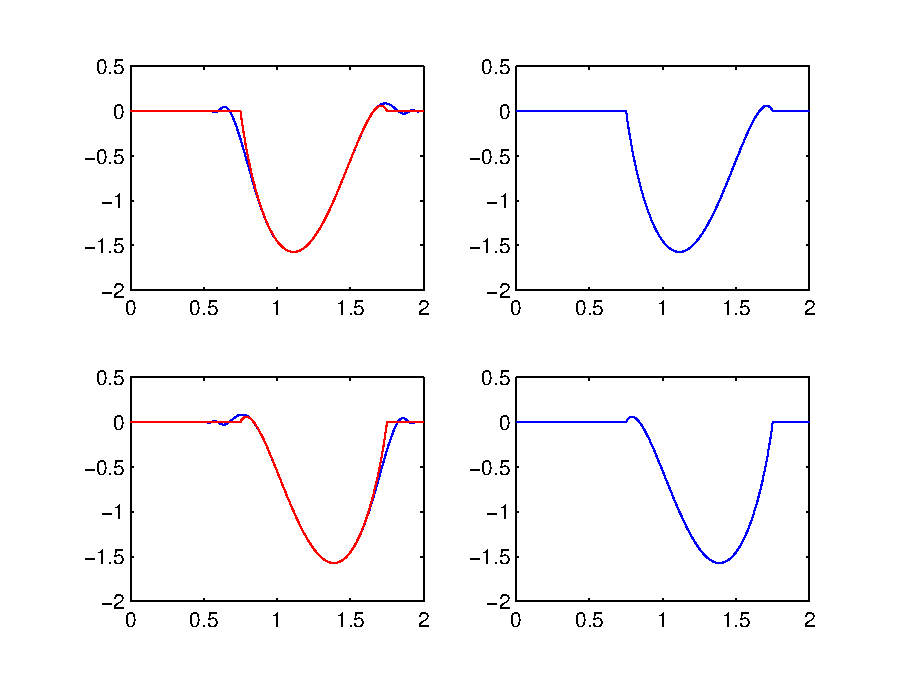
\includegraphics[width=0.8\textwidth]{./graphic/pwave_kirchhoff.eps}
	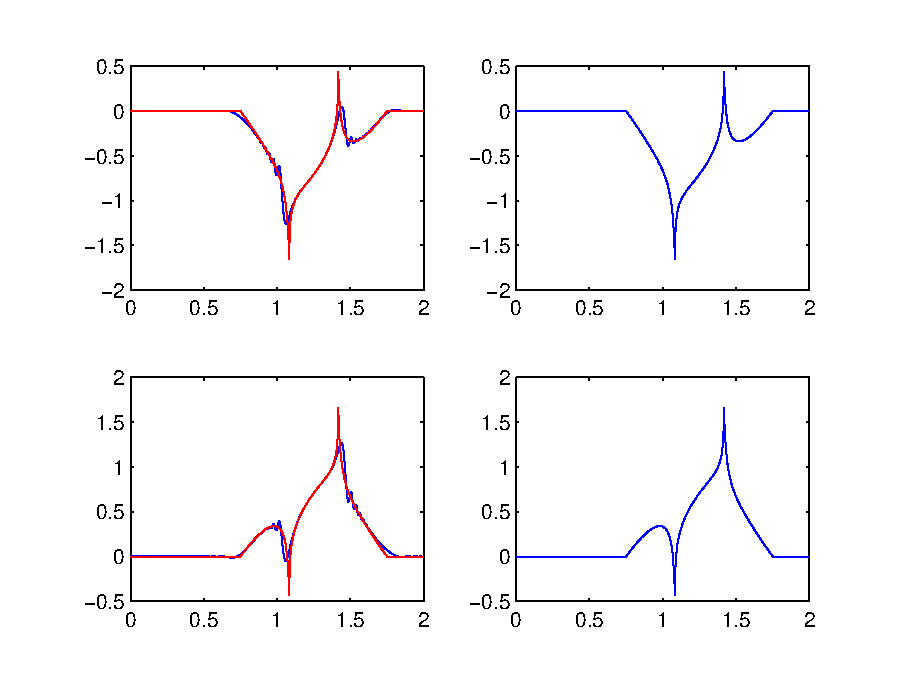
\includegraphics[width=0.8\textwidth]{./graphic/swave_kirchhoff.eps}	
	\caption{$\theta=pi/4$}\label{figure_2}
\end{figure}
\begin{figure}
	\centering
	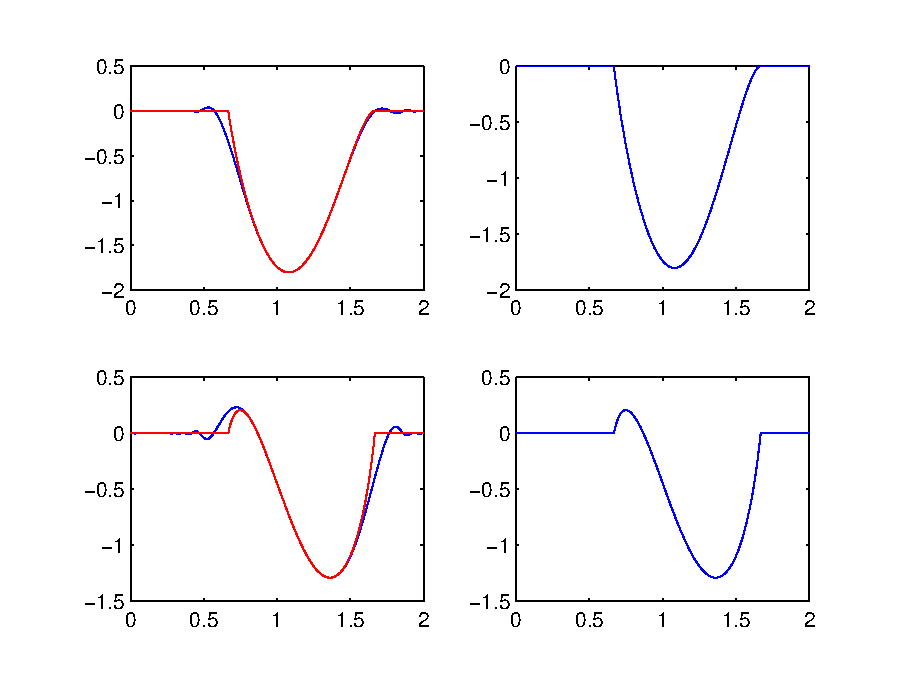
\includegraphics[width=0.8\textwidth]{./graphic/pwave_kirchhoffpi3.eps}
	\includegraphics[width=0.8\textwidth]{./graphic/swave_kirchhoffpi3.eps}	
	\caption{$\theta=\pi/3$}\label{figure_3}
\end{figure}

\section{Difference of solution of naviar equation in full-space and half-space,0105}

For any $0<\ep<1$, we consider the problem
\be {\label{elas_z1}}
\Delta_e u_1^\ep + (1+\i\ep)\omega^2 u_1^\ep=0 \qquad\mbox{\rm in } \R^2_+\bks \bar{D}\\
u_1^\ep= g \ \ \ \ \mbox{\rm on } \Ga_D  \label{elas_zbd}\\
\sigma(u_\eps^1)e_2=0 \ \ \ \ \mbox{\rm on} \Ga_0 \label{elas_zb0}
\ee
and
\be {\label{elas_z2}}
\Delta_e u_2^\ep + (1+\i\ep)\omega^2 u_2^\ep=0 \qquad\mbox{\rm in } \R^2\bks \bar{D}\\
u_2^\ep= g \ \ \ \ \mbox{\rm on } \Ga_D  \label{elas_zbd2}
\ee
Let $w^\ep(x)$ be the solution of the problem:
\be {\label{elas_z3}}
\Delta_e w^\ep + (1+\i\ep)\omega^2 w^\ep=0 \qquad\mbox{\rm in } \R^2_+\\
\sigma(w^\ep)e_2=-\sigma(u_2^\ep)e_2 \ \ \ \ \mbox{\rm on} \Ga_0 \label{elas_zb01}
\ee
Then $u^\ep_1-u^\ep_2-w^\ep$ satisfies (\ref{elas_z1}),(\ref{elas_zb0}) with the boundary condition $u^\ep_1-u^\ep_2-w^\ep=-w^\ep$ on $\Gamma_D$. Thus by the limiting absorption principle, we have
\be\label{diff1}
\|T_x^\nu(u^\ep_1-u^\ep_2)\|_{H^{-1/2}(\Gamma_D)}&\leq& C(\| w^\ep\|_{H^{1/2}(\Gamma_D)}+|T_x^\nu(w^\ep)\|_{H^{-1/2}(\Gamma_D)})\\
&\leq&C \max_{x\in D}(|w^\ep(x)|+d_D|\nabla w^\ep(x|)
\ee
where C is indepandent of $\ep,\om$. By the integral representation formula we have for any $z\in\Ga_0$
\be
u_2^\ep(z)=\int_{\Gamma_D}(T^{\nu}_y \Phi^\ep(y,z))^Tu_2^\ep(y)-\Phi^\ep(z,y)(T^{\nu}_y u_2^\ep(y)) ds(y)
\ee
which yields by using the integral representation again that for $x\in D$
\be
w^\ep(x)=\int_{\Ga_0} N^\ep(x,z)(T_z^{e_2}u_2^\ep(z))ds(z)\\
=\int_{\Gamma_D}ds(y)\int_{\Ga_0} N^\ep(x,z)(T_z^{e_2}((T^{\nu}_y \Phi^\ep(y,z))^T))ds(z)\\
-\int_{\Gamma_D}v^\ep(x,y)(T^{\nu}_y u_2^\ep(y))ds(y)\\
=\int_{\Gamma_D}ds(y)\int_{\Ga_0} N^\ep(x,z)(T_z^{e_2}( \Phi^\ep(y,z)^T(T^{\nu}_y)^T)ds(z)\\
-\int_{\Gamma_D}v^\ep(x,y)(T^{\nu}_y u_2^\ep(y))ds(y)\\
=\int_{\Gamma_D}ds(y)\int_{\Ga_0} N^\ep(x,z)(T^{\nu}_y(T_z^{e_2} \Phi^\ep(z,y))^T)^T ds(z)\\
-\int_{\Gamma_D}v^\ep(x,y)(T^{\nu}_y u_2^\ep(y))ds(y)\\
=\int_{\Gamma_D}(T^{\nu}_y( v^\ep(x,y))^T)^T u_2^\ep(y)
-v^\ep(x,y)(T^{\nu}_y u_2^\ep(y))ds(y)
\ee
where
\be
v^\ep(x,y)=\int_{\Ga_0} N^\ep(x,z)(T_z^{e_2}\Phi^\ep(z,y))ds(z)
\ee
Since $\|T_x^\nu(u^\ep_2)\|_{H^{-1/2}(\Gamma_D)}\leq C \|g\|_{H^{1/2}(\Gamma_D)}$, we obtain
\be
|w^\ep(x)|\leq C \|g\|_{H^{1/2}(\Gamma_D)}\max_{x\in D}(|v^\ep(x,y)|+d_D|\nabla_yv^\ep(x,y)|)
\ee
and
\be
|\nabla w^\ep(x)|\leq C \|g\|_{H^{1/2}(\Gamma_D)}\max_{x\in D}(|\nabla_x v^\ep(x,y)|+d_D|\nabla_x\nabla_yv^\ep(x,y)|)
\ee
By (\ref{diff1}) and letting $\ep\to0^+$, we have 
\be\label{diff2}
\|T_x^\nu(u_1-u_2)\|_{H^{-1/2}(\Gamma_D)}
\leq C\|g\|_{H^{1/2}(\Gamma_D)}\max_{x\in D}\lim_{\ep\to0^+}(|v^\ep(x,y)|\\
+d_D|\nabla_y v^\ep(x,y)|+d_D|\nabla_x v^\ep(x,y)|+d_D^2|\nabla_x\nabla_yv^\ep(x,y)|)
\ee
where $u_1$ is the scattering solution in the half-space and $u_2$ in the full-space. Now, it turns to estimate $v^\ep(x,y)$. Applying the Fourier transformation to the first horizontal variable of $N^\ep(z,x)$ and$T_z^{e_2}\Phi^\ep(z,y)$, we have 
\ben
\hspace{-2cm}
\mathcal{F}[N^\ep](\xi,0;x)
=\frac{\i}{\mu\delta(\xi)} \Bigg[ \Bigg(
\begin{array}{cc}
	2\xi^2\mu_s & -2\xi\mu_s\mu_p\\
	-\xi\beta & \mu_p\beta
\end{array} \Bigg)e^{\i\mu_p x_2}
+ \Bigg(
\begin{array}{cc}
	\mu_s\beta & \xi\beta \\
	2\xi\mu_s\mu_p & 2\xi^2\mu_p
\end{array} \Bigg)e^{\i\mu_s x_2} \Bigg]e^{-\i\xi x_1} \\
\een
\ben \hspace{-2cm}
\mathcal{F}[T_z^{e_2}\Phi^\ep](\xi,0;y)=\frac{\mu}{2\omega^2}
\Bigg[
\Bigg( \begin{array}{cc}
	2\xi^2 & -2\xi\mu_p\\
	-\frac{\beta\xi}{\mu_p} & \beta
\end{array} \Bigg) e^{\i\mu_py_2}+
 \Bigg( \begin{array}{cc}
	\beta & \frac{\xi\beta}{\mu_s} \\
	2\xi\mu_s & 2\xi^2
\end{array} \Bigg)e^{\i\mu_s y_2}  \Bigg]e^{-\i\xi y_1}
\een
Using Parseval identity combined with above two formula, we have
\ben
\lim_{\ep\to0^+}v^\ep(x,y)=\lim_{\ep\to0^+}\int_{\R}\mathcal{F}[N^\ep](\xi,0;x)^T\mathcal{F}[T_z^{e_2}\Phi^\ep](-\xi,0;y)d\xi
\een
\begin{lem}
	For any $x,y\in D$, let
	\ben
	p(x,y)=\lim_{\ep\to0^+}p^\ep(x,y):=\lim_{\ep\to0^+}\int_\R \frac{f(\mu^\ep_p,\mu^\ep_s,\xi)}{\delta^\ep(\xi)}e^{\i\mu^\ep_\alpha x_2+\i \mu^\ep_\beta y_2+\i \xi(y_1-x_1)}d\xi
	\een
	where $f(a,b,c)$ is a homogeneous fifth order polynomial with repect to a,b,c and $\alpha=s,p$, $\beta=s,p$.Then there exists a constant $C>0$ only depandent on $\kappa$ such that
	\ben\hspace{-2.5cm}
	|p(x,y)|+k_s^{-1}|\nabla_x p(x,y)|+k_s^{-1}|\nabla_y p(x,y)|+k_s^{-2}|\nabla_x\nabla_y p(x,y)|\leq C((k_s h)^{-1/2}+e^{-\sqrt{k_R^2-k_s^2}h})
	\een
	uniformly for $x,y\in D$.
\end{lem}
\debproof
Without loss of generality, we assume $k_\alpha\leq k_\beta$. Then we can divide $p(x,y)$ into two parts:
\ben
p(x,y)&=&\lim_{\ep\to0^+}\int_{I_1}+\int_{I_2}\frac{f(\mu^\ep_p,\mu^\ep_s,\xi)}{(k^\ep_\alpha)^2\delta^\ep(\xi)}e^{\i\mu^\ep_\alpha x_2+\i \mu^\ep_\beta y_2+\i \xi(y_1-x_1)}d\xi\\
&=&\int_{I_1}\frac{f(\mu_p,\mu_s,\xi)}{k^2_\alpha\delta(\xi)}e^{\i\mu_\alpha x_2+\i \mu_\beta y_2+\i \xi(y_1-x_1)}d\xi\\
&+&\lim_{\ep\to0^+}\int_{I_2}\frac{f(\mu^\ep_p,\mu^\ep_s,\xi)}{(k^\ep_\alpha)^2\delta^\ep(\xi)}e^{\i\mu^\ep_\alpha x_2+\i \mu^\ep_\beta y_2+\i \xi(y_1-x_1)}d\xi\\
&=&p_1(x,y)+p_2(x,y)
\een
where $I_1=(-k_\alpha,k_\alpha)$, $I_2=(-2k_R+k_\alpha,k_\alpha)\cup(k_\alpha,2k_R-k_\alpha)$ and $I_2=R\bks[-k_\alpha,k_\alpha]$. Substituting $\xi=k_\alpha t$ into $p_1(x,y)$, we get
\ben
p_1(x,y)=\int_{-1}^{1}\frac{ f(\mu_p(k_\alpha t),\mu_s(k_\alpha t),k_\alpha t)}{k_\alpha \delta(k_\alpha t)}e^{\i k_\alpha x_2(\sqrt{1-t^2}+\tau \sqrt{\varsigma^2-t^2} +\gamma t)}dt
\een
where $\tau=y_2/x_2$, $\varsigma=k_\beta/k_\alpha$ and $\gamma=(y_1-x_1)/x_2$. It is easy to see that the phase function $\phi(t)=\sqrt{1-t^2}+\tau \sqrt{\varsigma^2-t^2} +\gamma t$ satifies $|\phi''(t)|\geq 1/(1-t^2)^{3/2}\geq1$ for $t\in(-1,1)$. Then we can obtain $|p_1(x,y)|\leq C 1/(k_s h)^{1/2}$ by lemma \ref{van}.

For $p_2(x,y)$, by changing the integration path and using same argument as in the proof of estimate for psf, we can easily obtain:
\ben
|p_2(x,y)|\leq C(\frac{1}{k_sh}+e^{-\sqrt{k_R^2-k_s^2}}h)
\een
This completes the proof of the esitmate for $|p(x,y)|$. The other estimates can be proved by a similar argument. We omit the details
\finproof
\begin{lem}
	For any $x,y\in D$, let
	\ben
	p(x,y)=\lim_{\ep\to0^+}p^\ep(x,y):=\lim_{\ep\to0^+}\int_\R \frac{f(\mu^\ep_p,\mu^\ep_s,\xi)}{\delta^\ep(\xi)}e^{\i\mu^\ep_\alpha x_2+\i \mu^\ep_\beta y_2+\i \xi(y_1-x_1)}d\xi
	\een
	where $f(a,b,c)$ is a homogeneous fifth order polynomial with repect to a,b,c and $\alpha=s,p$, $\beta=s,p$.Then there exists a constant $C>0$ only depandent on $\kappa$ such that
	\ben\hspace{-3cm}
	|p(x,y)|+k_s^{-1}|\nabla_x p(x,y)|+k_s^{-1}|\nabla_y p(x,y)|+k_s^{-2}|\nabla_x\nabla_y p(x,y)|\leq C(1+k_s d_D)((k_s h)^{-1/2}+e^{-\sqrt{k_R^2-k_s^2}h})
	\een
	uniformly for $x,y\in D$.
\end{lem}
\debproof
Without loss of generality, we assume $k_\alpha\leq k_\beta$. Then we can divide $p(x,y)$ into four parts:
\ben
p(x,y)&=&\lim_{\ep\to0^+}\int_{I_1}+\int_{I_2}+\int_{I_3}\frac{f(\mu^\ep_p,\mu^\ep_s,\xi)}{(k^\ep_\alpha)^2\delta^\ep(\xi)}e^{\i\mu^\ep_\alpha x_2+\i \mu^\ep_\beta y_2+\i \xi(y_1-x_1)}d\xi\\
&=&\int_{I_1}+\mathrm{PV}\int_{I_2}+\int_{I_3}\frac{f(\mu_p,\mu_s,\xi)}{k^2_\alpha\delta(\xi)}e^{\i\mu_\alpha x_2+\i \mu_\beta y_2+\i \xi(y_1-x_1)}d\xi\\
&+&\i\pi(\frac{f(\mu_p(k_R),\mu_s(k_R),k_R)}{k^2_\alpha\delta'(k_R)}e^{\i\mu_\alpha(k_R) x_2+\i \mu_\beta(k_R) y_2+\i k_R(y_1-x_1)}\\
&-&\frac{f(\mu_p(k_R),\mu_s(k_R),-k_R)}{k^2_\alpha\delta'(-k_R)}e^{\i\mu_\alpha(k_R) x_2+\i \mu_\beta(k_R) y_2-\i k_R(y_1-x_1)})\\
:&=&p_1(x,y)+p_2(x,y)+p_3(x,y)+p_4(x,y)
\een
where $I_1=(-k_\alpha,k_\alpha)$, $I_2=(-2k_R+k_\alpha,k_\alpha)\cup(k_\alpha,2k_R-k_\alpha)$ and $I_3=R\bks[-2k_R+k_\alpha,2k_R-k_\alpha]$. Substituting $\xi=k_\alpha t$ into $p_1(x,y)$, we get
\ben
p_1(x,y)=\int_{-1}^{1}\frac{ f(\mu_p(k_\alpha t),\mu_s(k_\alpha t),k_\alpha t)}{k_\alpha \delta(k_\alpha t)}e^{\i k_\alpha x_2(\sqrt{1-t^2}+\tau \sqrt{\varsigma^2-t^2} +\gamma t)}dt
\een
where $\tau=y_2/x_2$, $\varsigma=k_\beta/k_\alpha$ and $\gamma=(y_1-x_1)/x_2$. It is easy to see that the phase function $\phi(t)=\sqrt{1-t^2}+\tau \sqrt{\varsigma^2-t^2} +\gamma t$ satifies $|\phi''(t)|\geq 1/(1-t^2)^{3/2}\geq1$ for $t\in(-1,1)$. Then we can obtain $|p_1(x,y)|\leq C 1/(k_s h)^{1/2}$ by lemma \ref{van}.

Let 
\ben
g_\pm(\xi)=\frac{f(\mu_p,\mu_s,\xi)(\xi\pm k_R)}{\delta(\xi)}e^{\i\mu_\alpha x_2+\i \mu_\beta y_2+\i \xi(y_1-x_1)}d\xi
\een
 Then by the definition of cauchy principle value, we have
\ben
p_2(x,y)=\int_{-2k_R+k_\alpha}^{-k_\alpha}\frac{g_-(\xi)-g_-(-k_R)}{x+k_R}d\xi+\int_{k_\alpha}^{2k_R-k_\alpha}\frac{g_+(\xi)-g_+(k_R)}{x-k_R}d\xi
\een
\finproof
\begin{figure}
	\centering
	\includegraphics[width=0.24\textwidth]{./graphic/peanut_2pi.eps}
	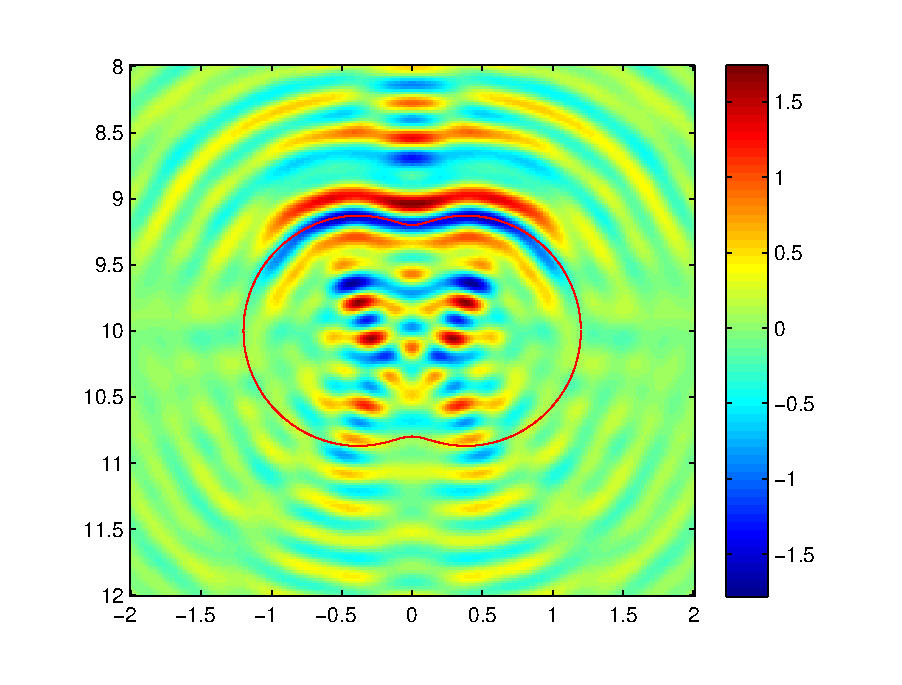
\includegraphics[width=0.24\textwidth]{./graphic/peanut_2pi_neumann.eps}
	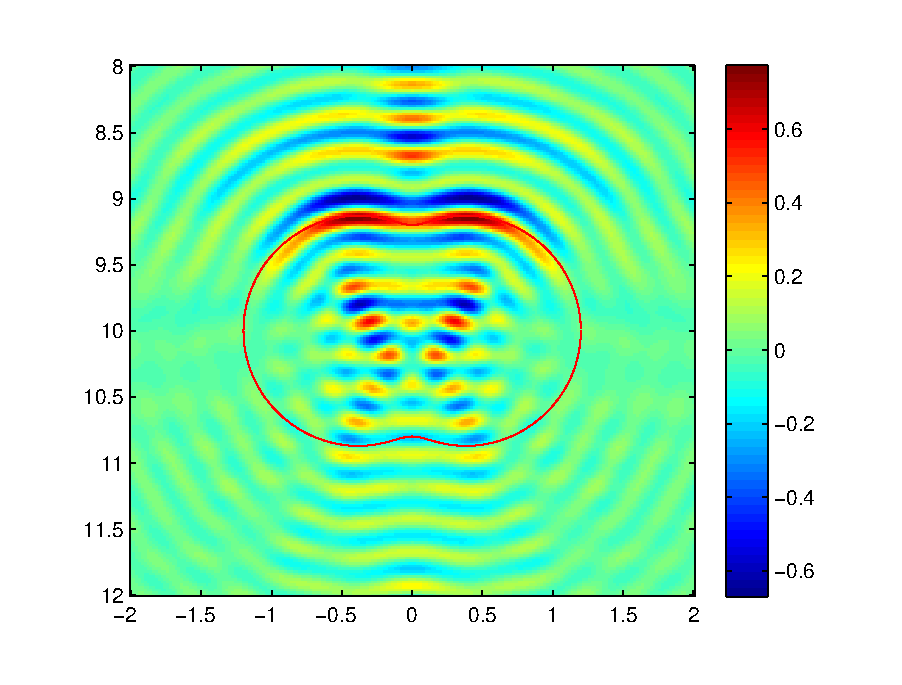
\includegraphics[width=0.24\textwidth]{./graphic/peanut_2pi_impedance_1.eps}
	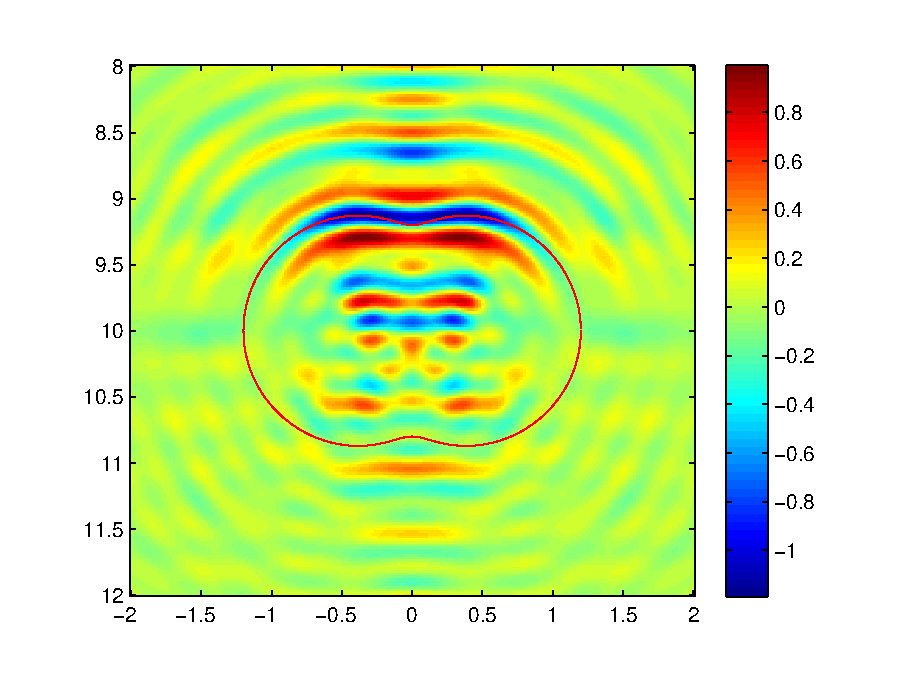
\includegraphics[width=0.24\textwidth]{./graphic/peanut_2pi_transmission.eps}
	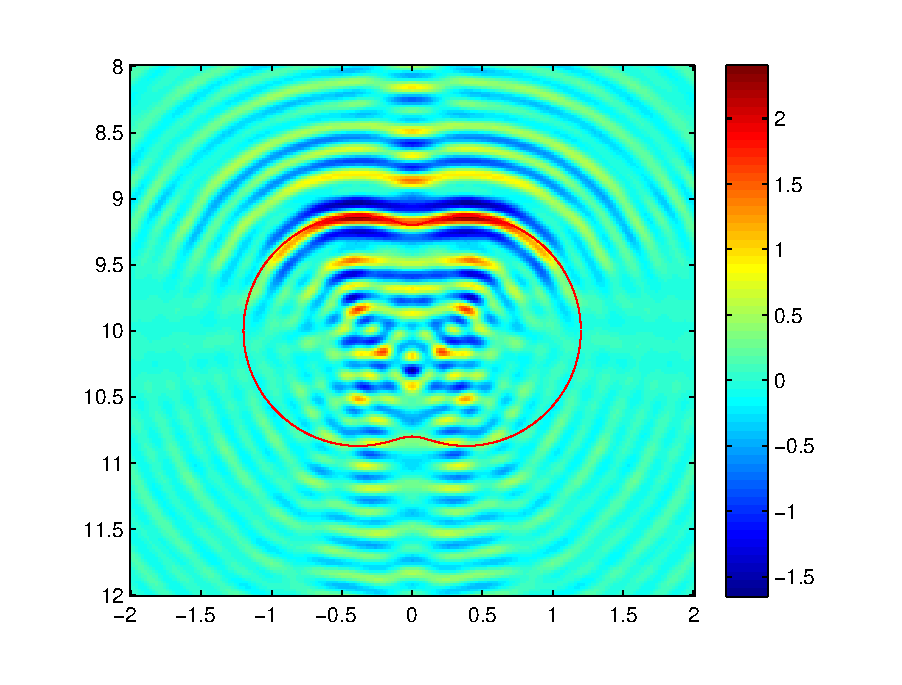
\includegraphics[width=0.24\textwidth]{./graphic/peanut_3pi.eps}
	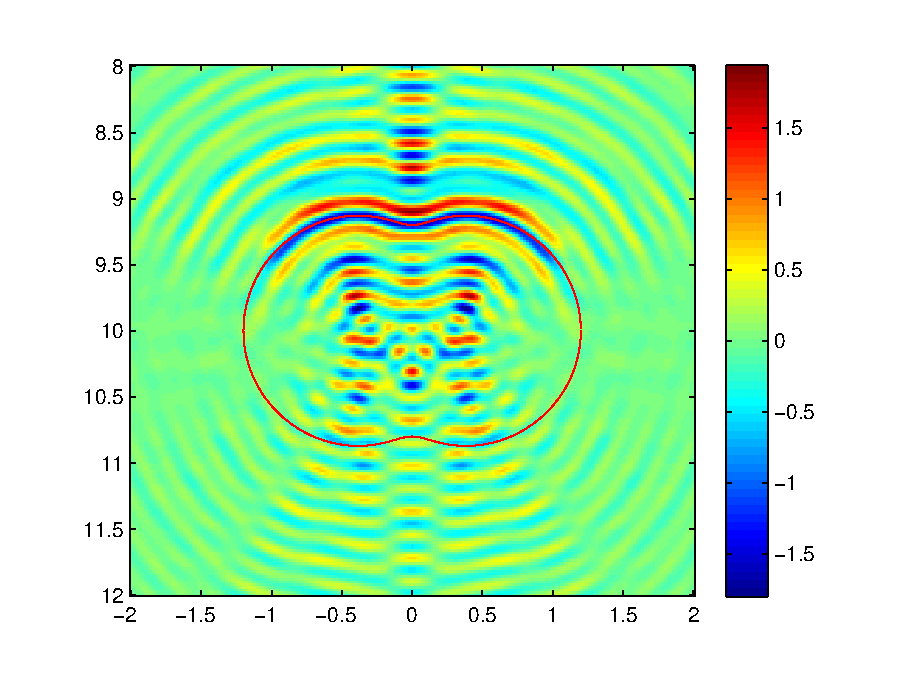
\includegraphics[width=0.24\textwidth]{./graphic/peanut_3pi_neumann.eps}
	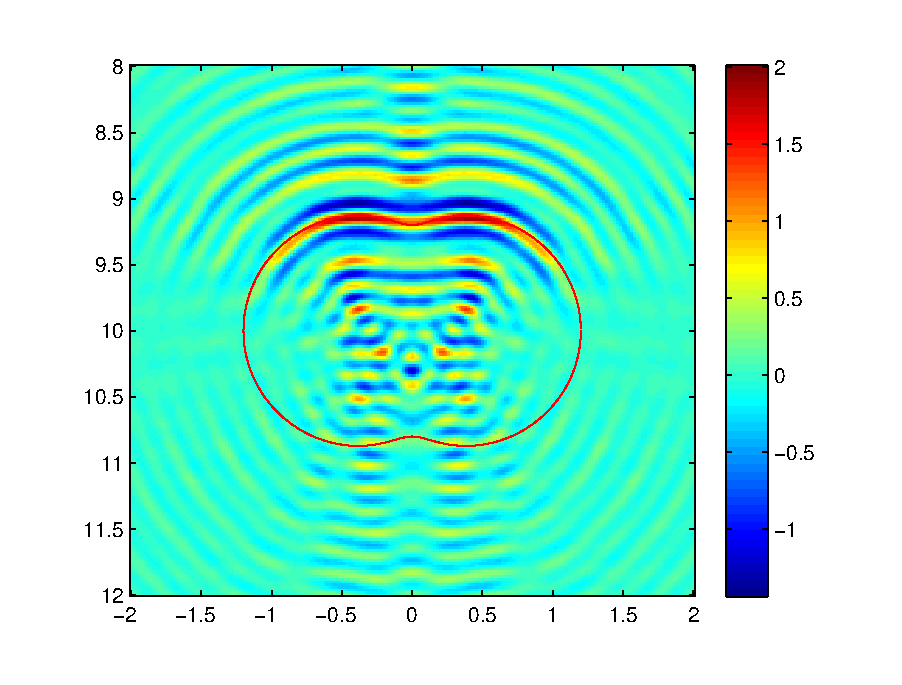
\includegraphics[width=0.24\textwidth]{./graphic/peanut_3pi_impedance_1.eps}
	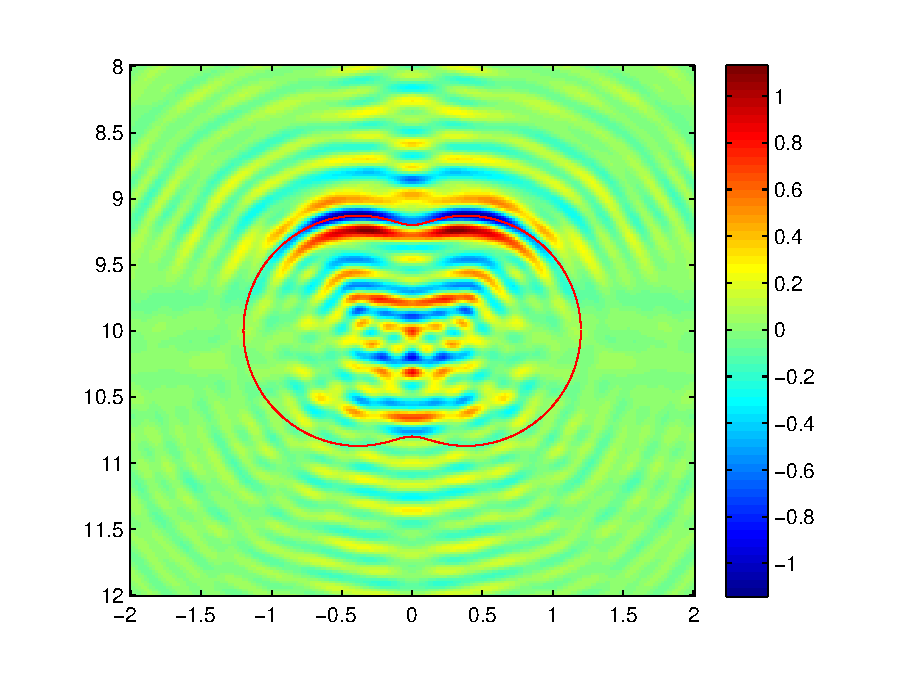
\includegraphics[width=0.24\textwidth]{./graphic/peanut_3pi_transmission.eps}
	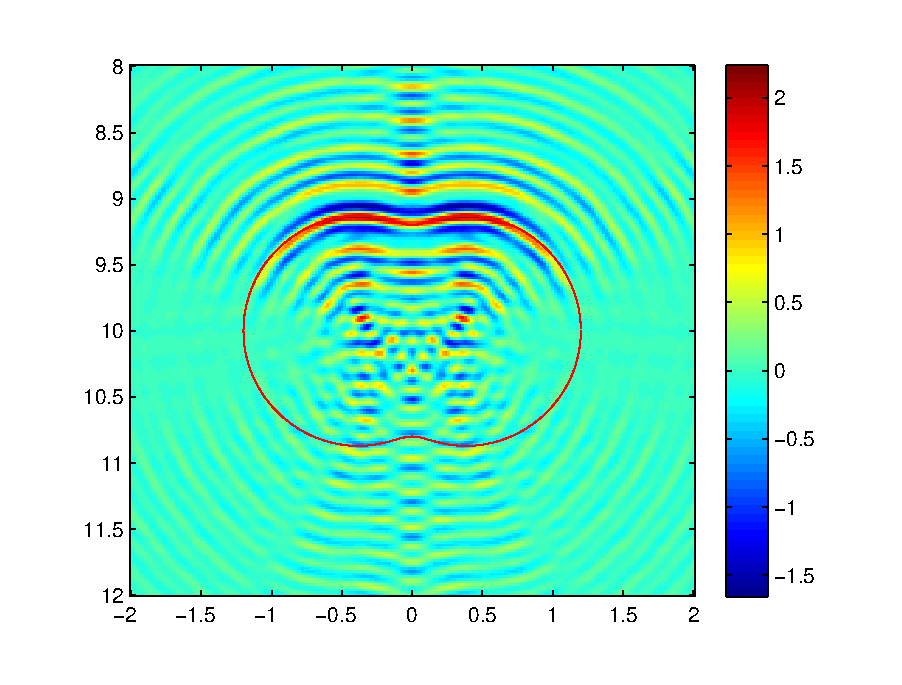
\includegraphics[width=0.24\textwidth]{./graphic/peanut_4pi.eps}
	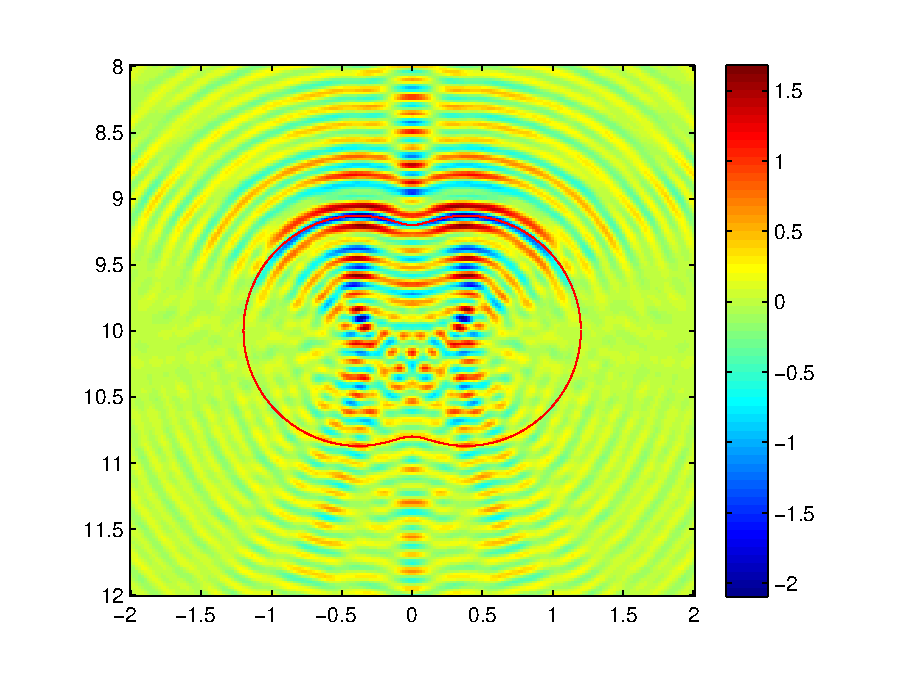
\includegraphics[width=0.24\textwidth]{./graphic/peanut_4pi_neumann.eps}
	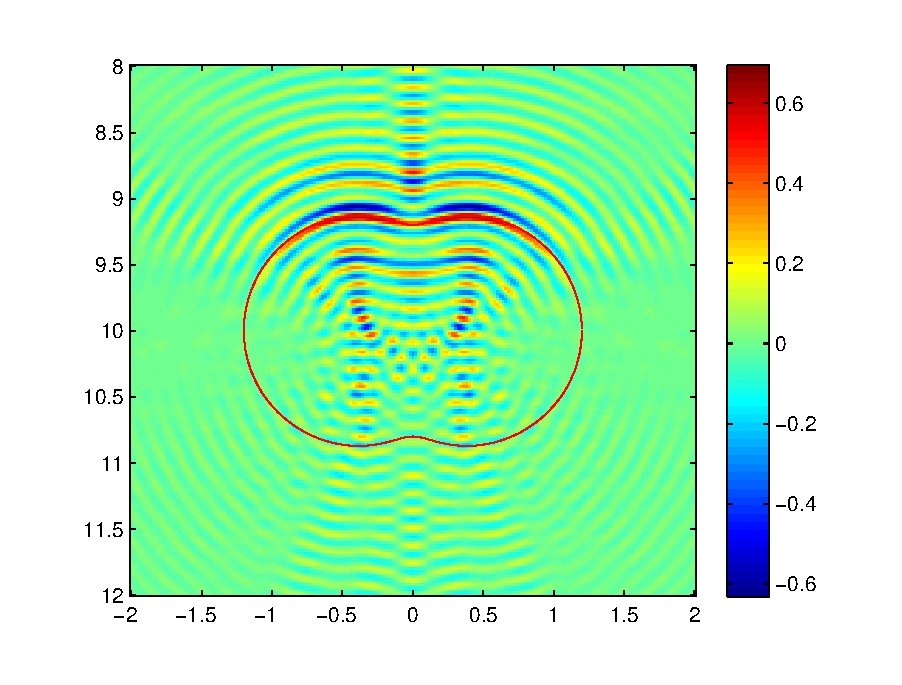
\includegraphics[width=0.24\textwidth]{./graphic/peanut_4pi_impedance_1.eps}
	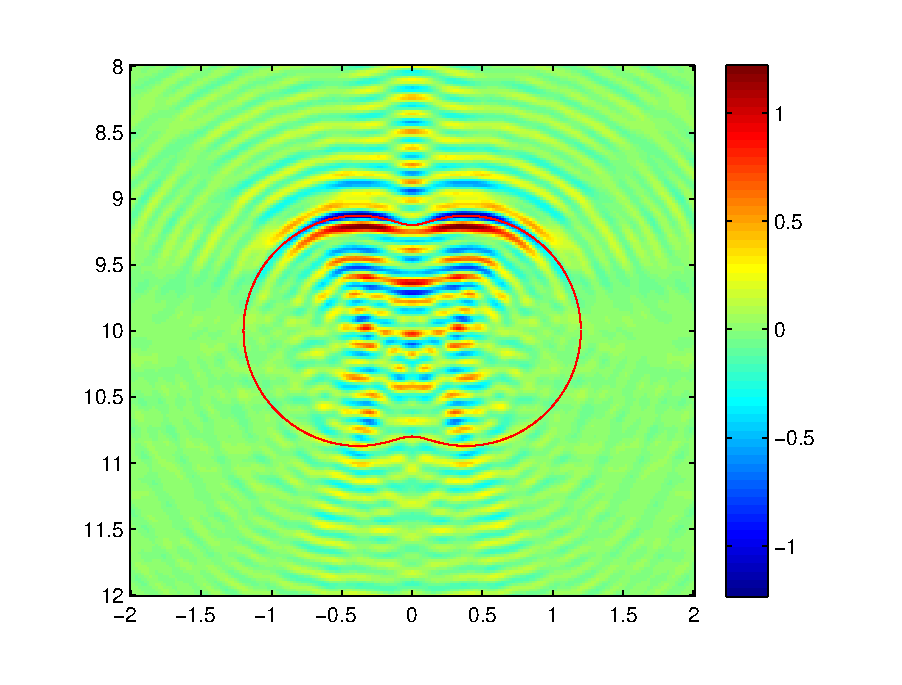
\includegraphics[width=0.24\textwidth]{./graphic/peanut_4pi_transmission.eps}
	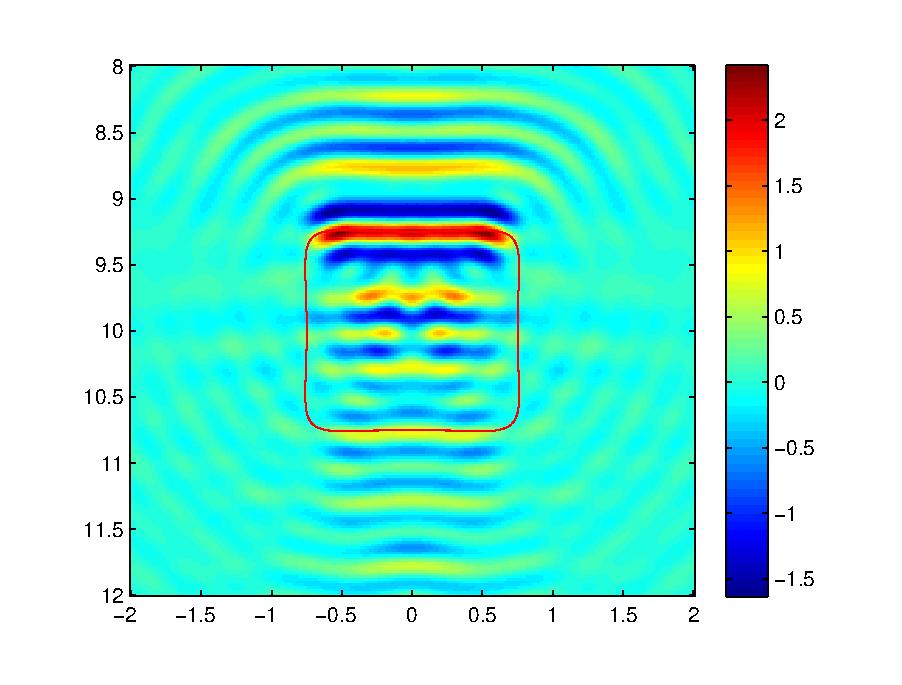
\includegraphics[width=0.24\textwidth]{./graphic/rectangle_2pi.eps}
	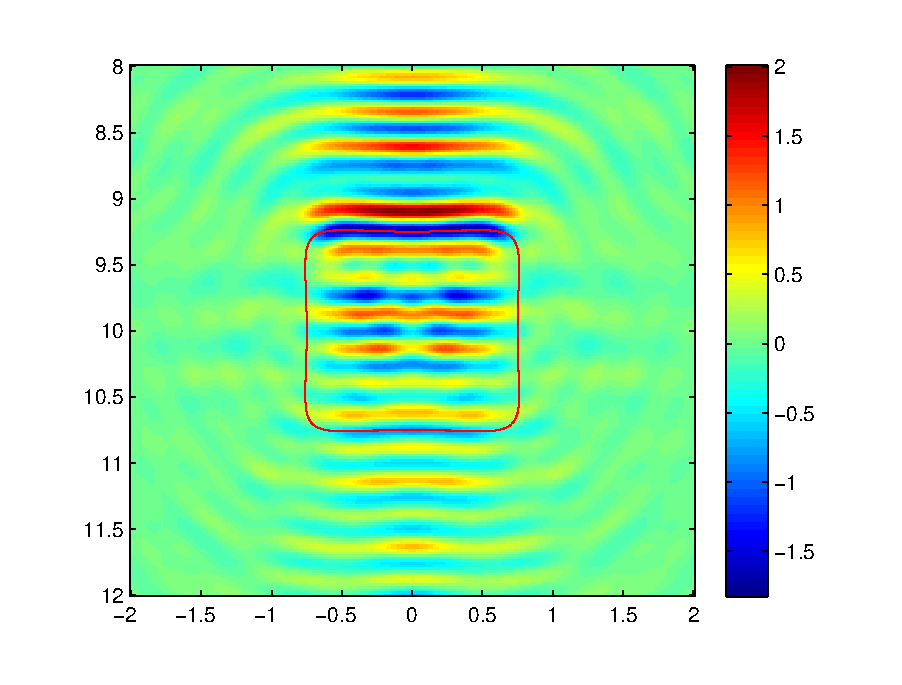
\includegraphics[width=0.24\textwidth]{./graphic/rectangle_2pi_neumann.eps}
	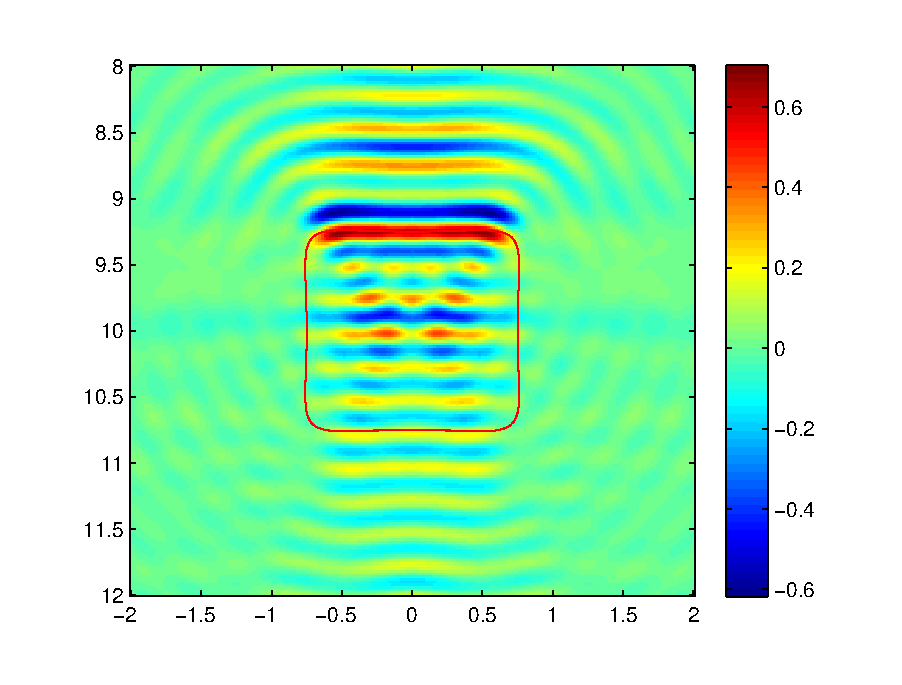
\includegraphics[width=0.24\textwidth]{./graphic/rectangle_2pi_impedance_1.eps}
	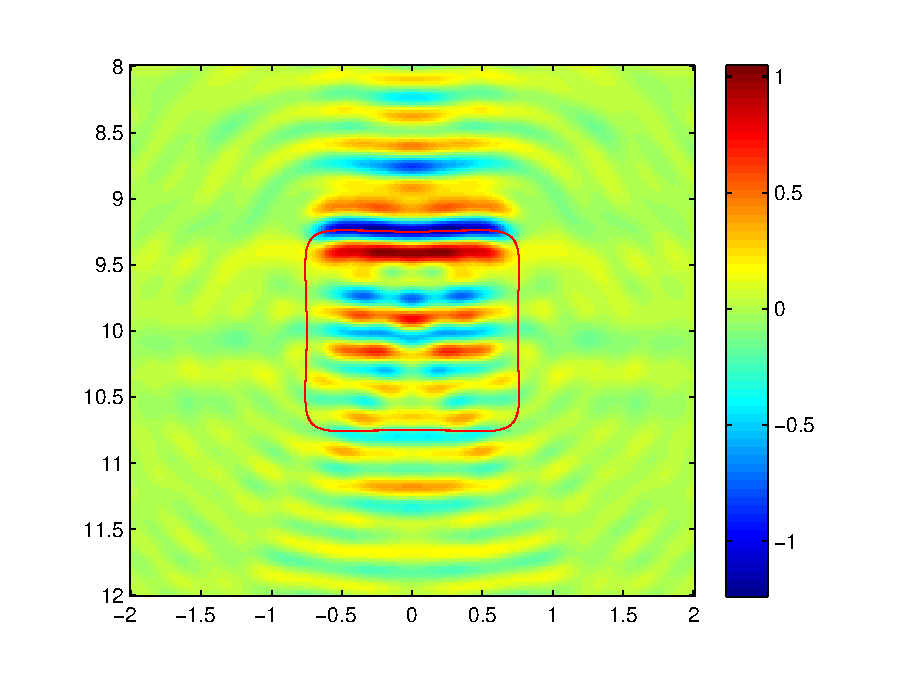
\includegraphics[width=0.24\textwidth]{./graphic/rectangle_2pi_transmission.eps}
	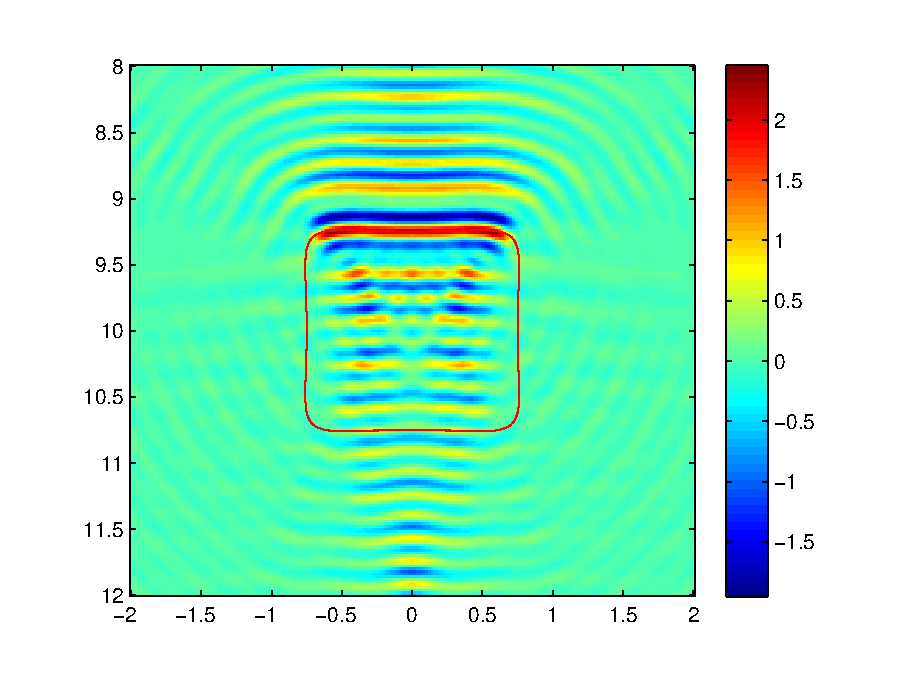
\includegraphics[width=0.24\textwidth]{./graphic/rectangle_3pi.eps}
	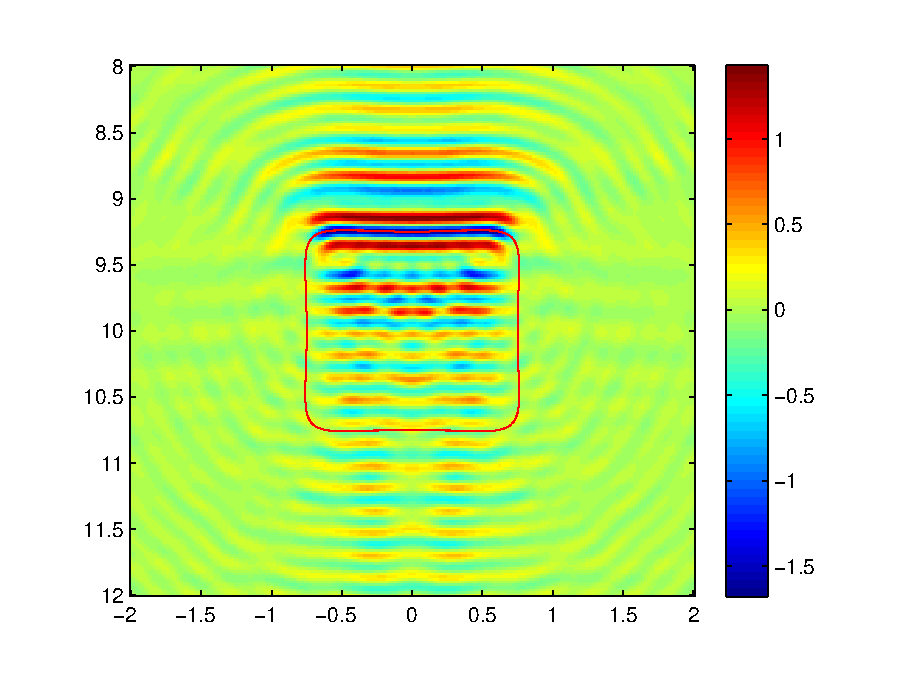
\includegraphics[width=0.24\textwidth]{./graphic/rectangle_3pi_neumann.eps}
	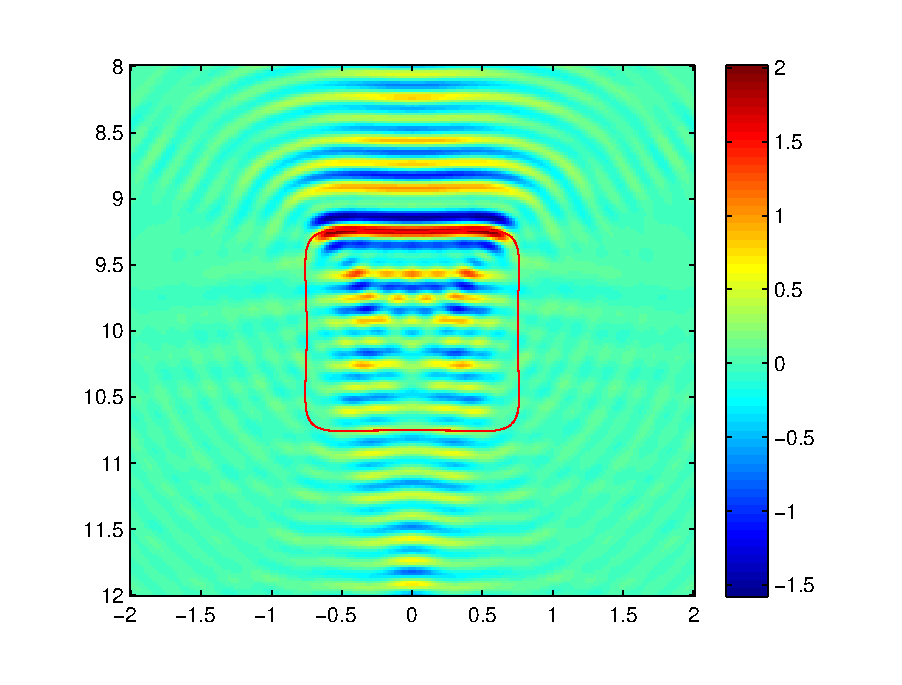
\includegraphics[width=0.24\textwidth]{./graphic/rectangle_3pi_impedance_1.eps}
	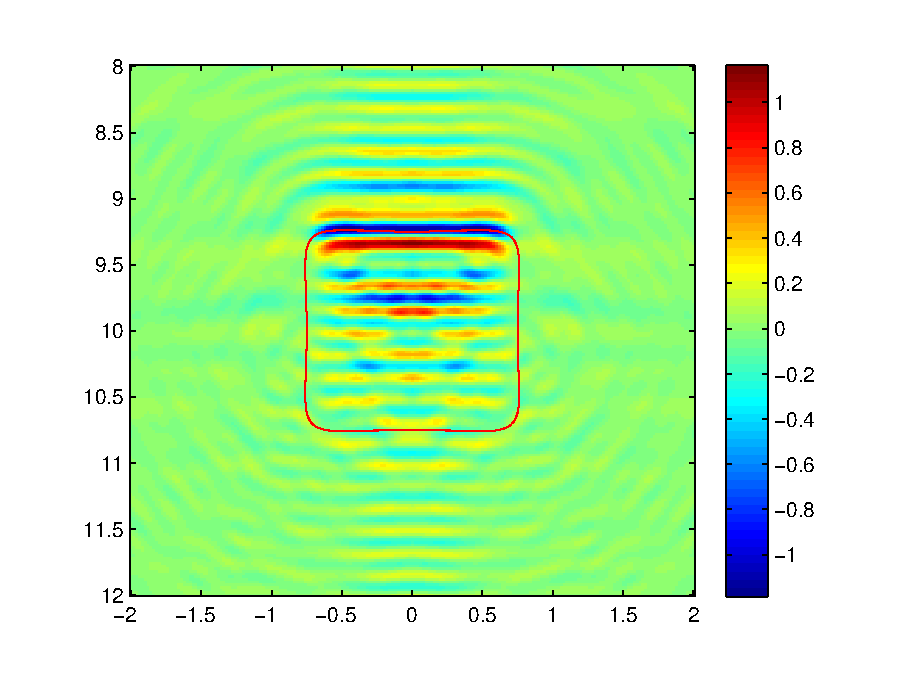
\includegraphics[width=0.24\textwidth]{./graphic/rectangle_3pi_transmission.eps}
	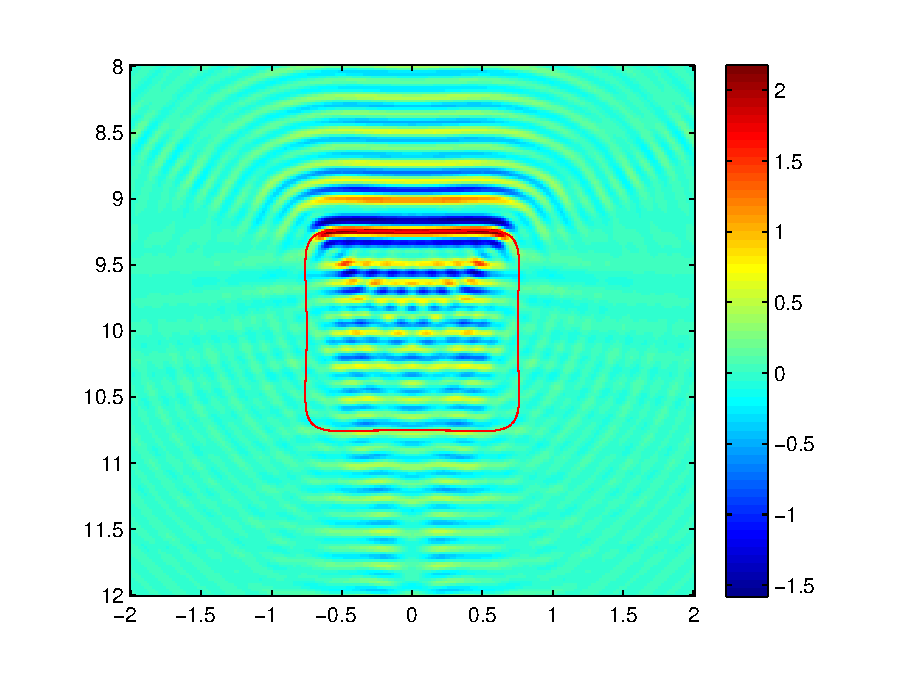
\includegraphics[width=0.24\textwidth]{./graphic/rectangle_4pi.eps}
	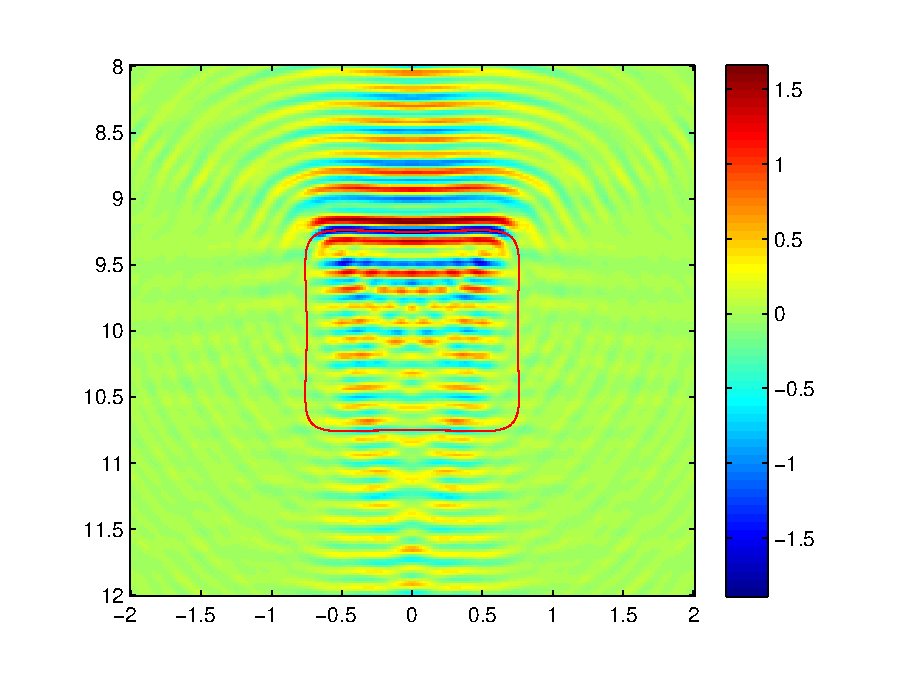
\includegraphics[width=0.24\textwidth]{./graphic/rectangle_4pi_neumann.eps}
	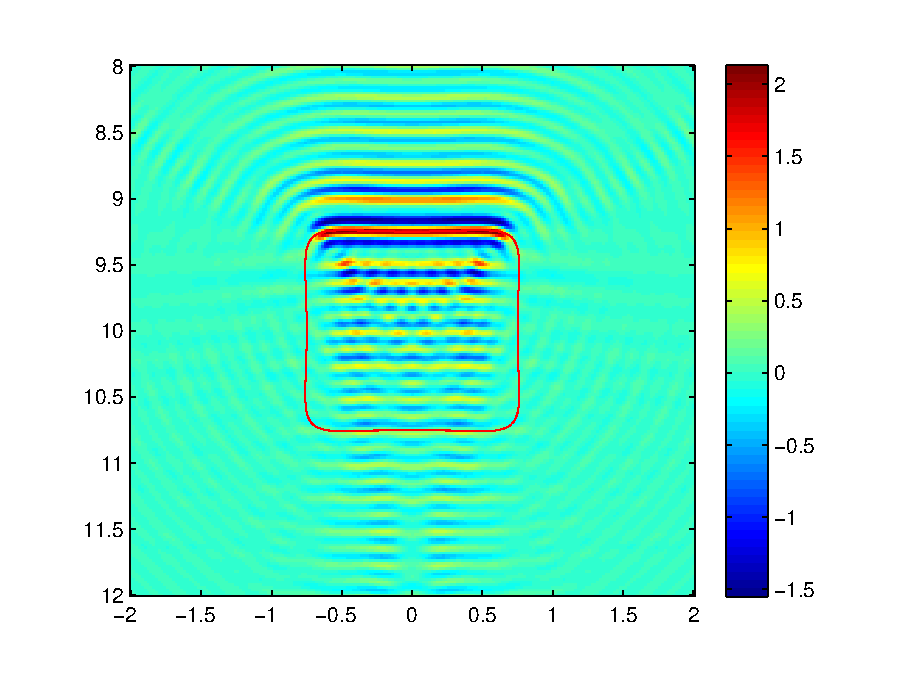
\includegraphics[width=0.24\textwidth]{./graphic/rectangle_4pi_impedance_1.eps}
	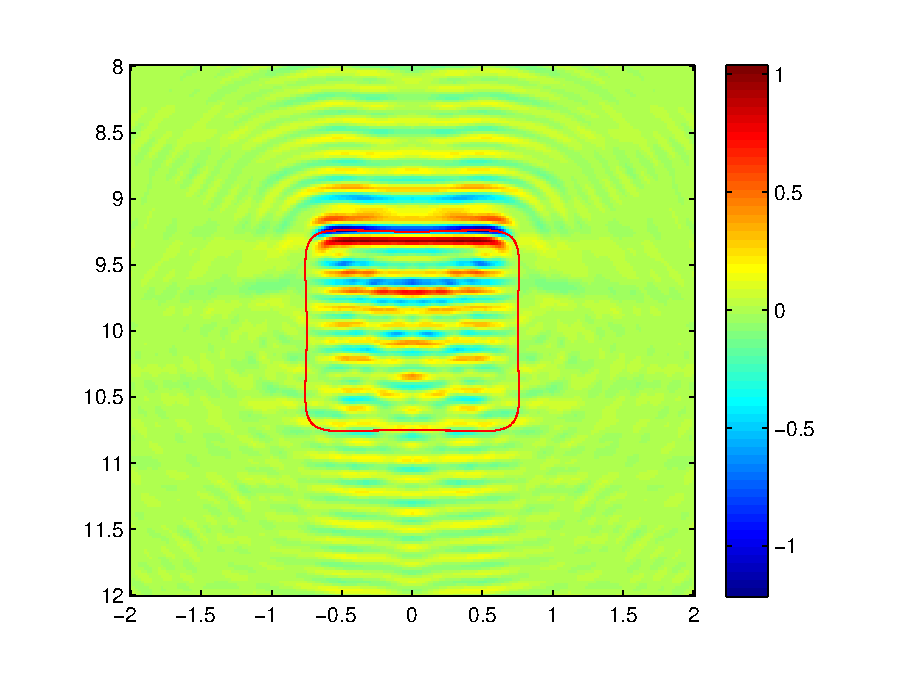
\includegraphics[width=0.24\textwidth]{./graphic/rectangle_4pi_transmission.eps}
	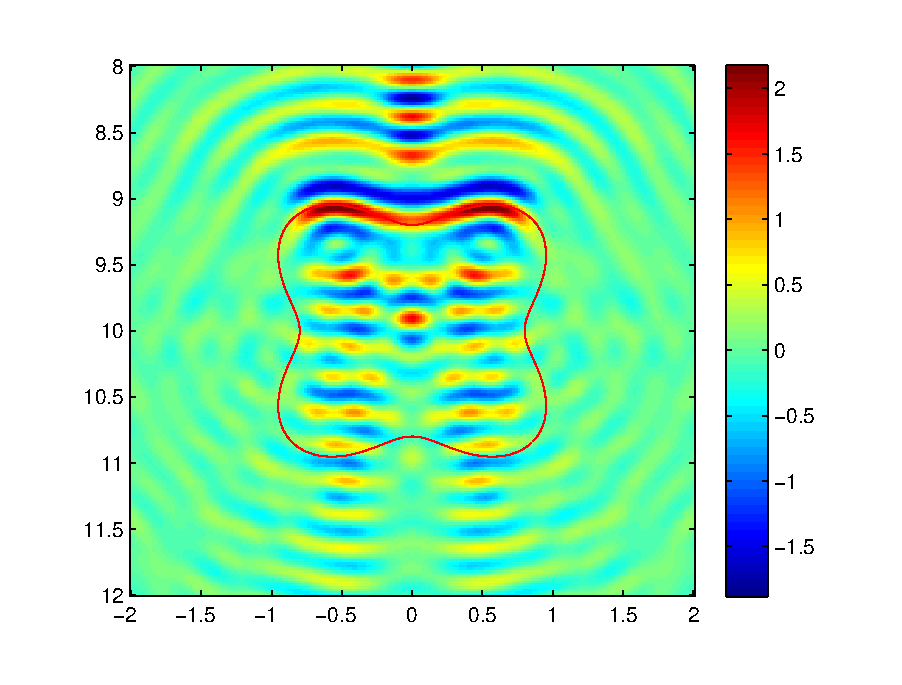
\includegraphics[width=0.24\textwidth]{./graphic/p_leaf_2pi.eps}
	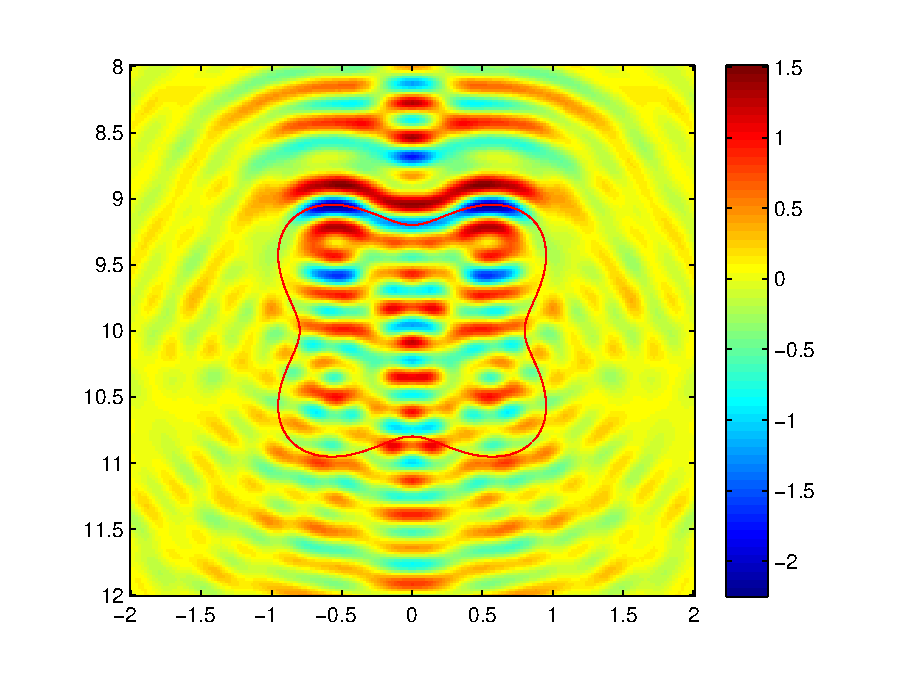
\includegraphics[width=0.24\textwidth]{./graphic/p_leaf_2pi_neumann.eps}
	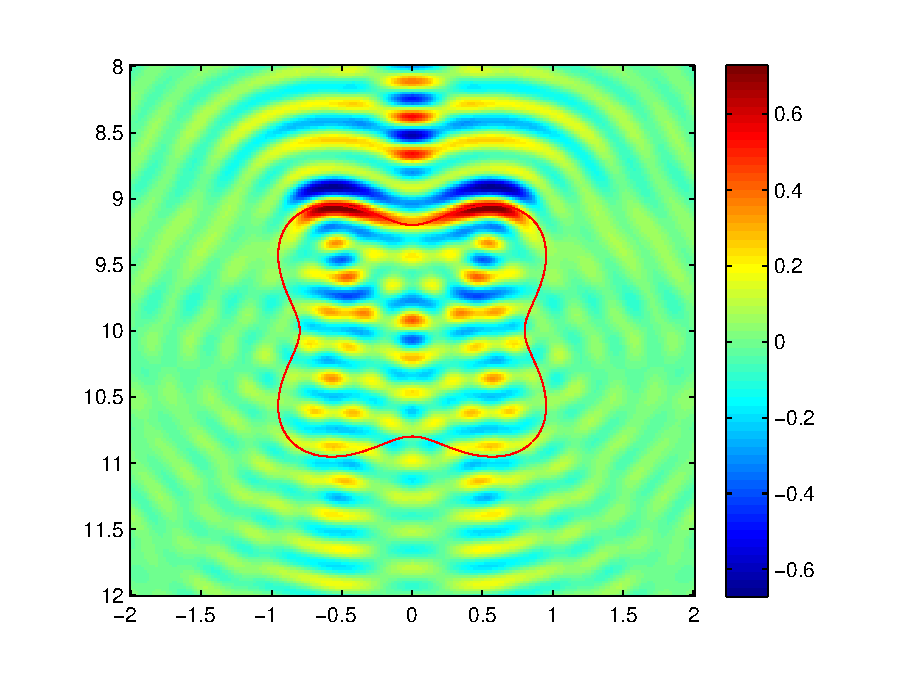
\includegraphics[width=0.24\textwidth]{./graphic/p_leaf_2pi_impedance_1.eps}
	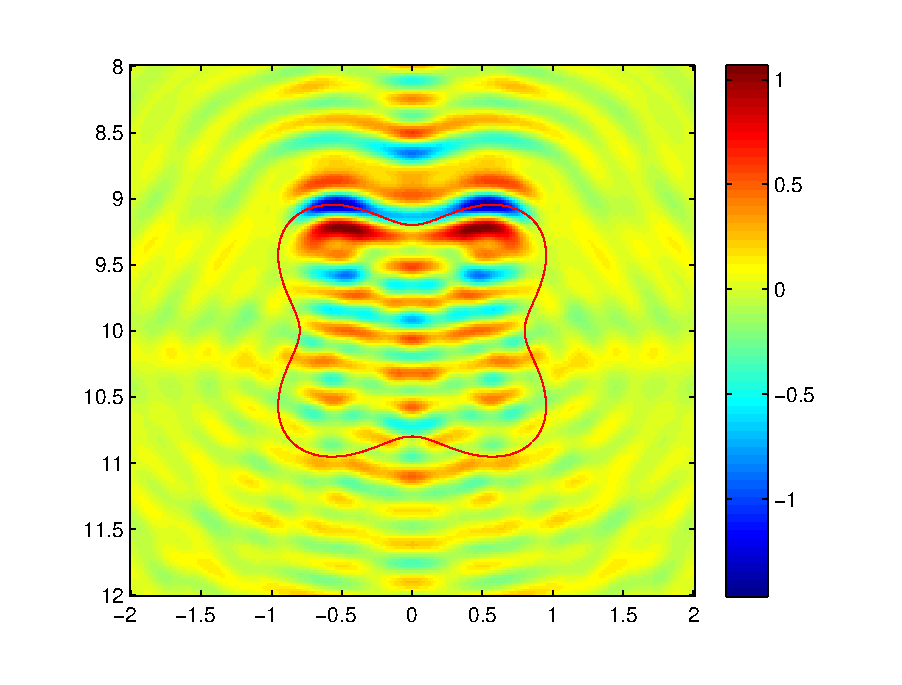
\includegraphics[width=0.24\textwidth]{./graphic/p_leaf_2pi_transmission.eps}
	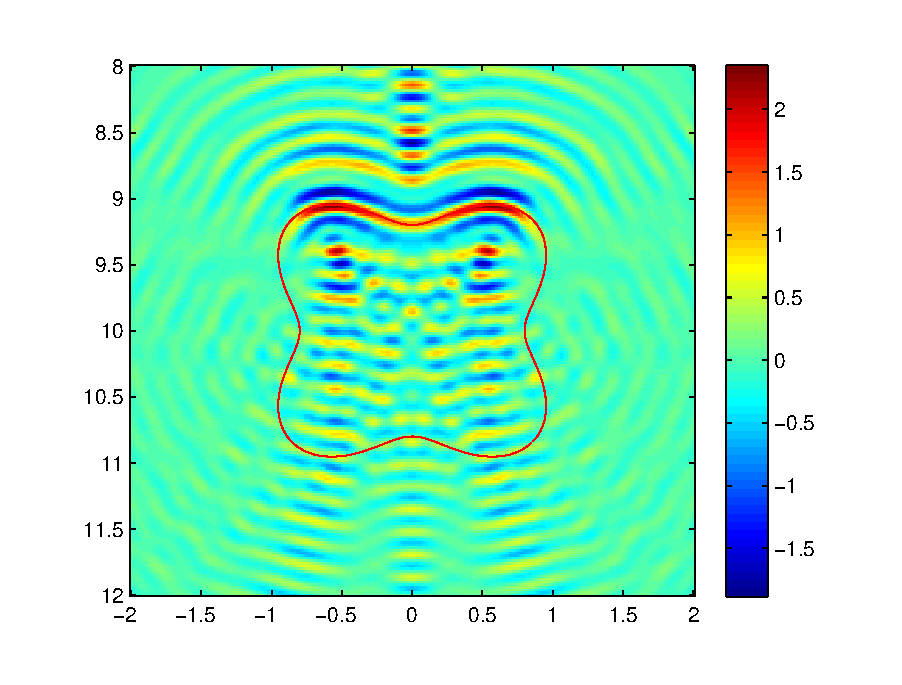
\includegraphics[width=0.24\textwidth]{./graphic/p_leaf_3pi.eps}
	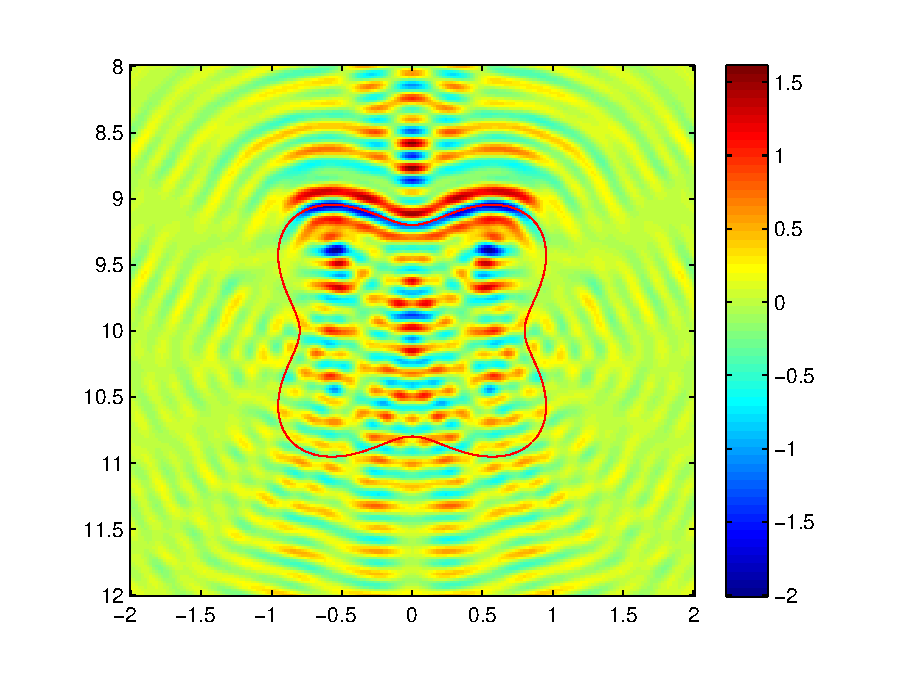
\includegraphics[width=0.24\textwidth]{./graphic/p_leaf_3pi_neumann.eps}
	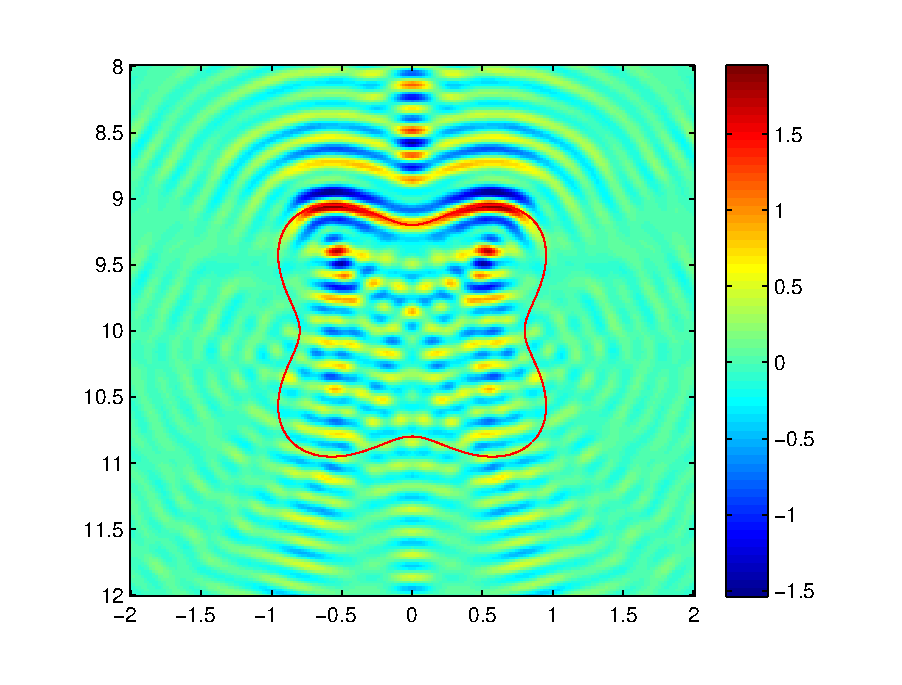
\includegraphics[width=0.24\textwidth]{./graphic/p_leaf_3pi_impedance_1.eps}
	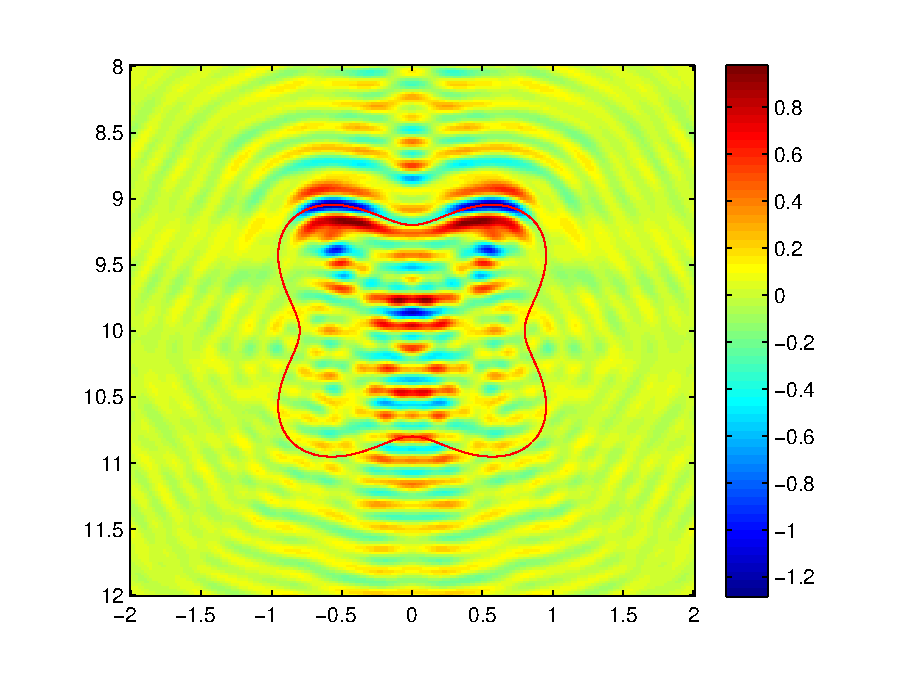
\includegraphics[width=0.24\textwidth]{./graphic/p_leaf_3pi_transmission.eps}
	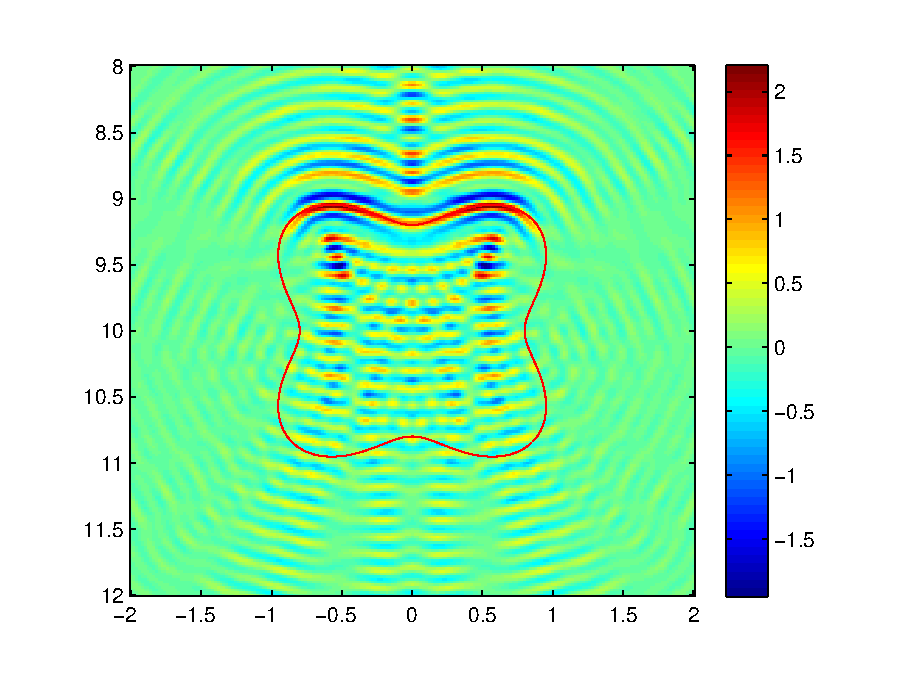
\includegraphics[width=0.24\textwidth]{./graphic/p_leaf_4pi.eps}
	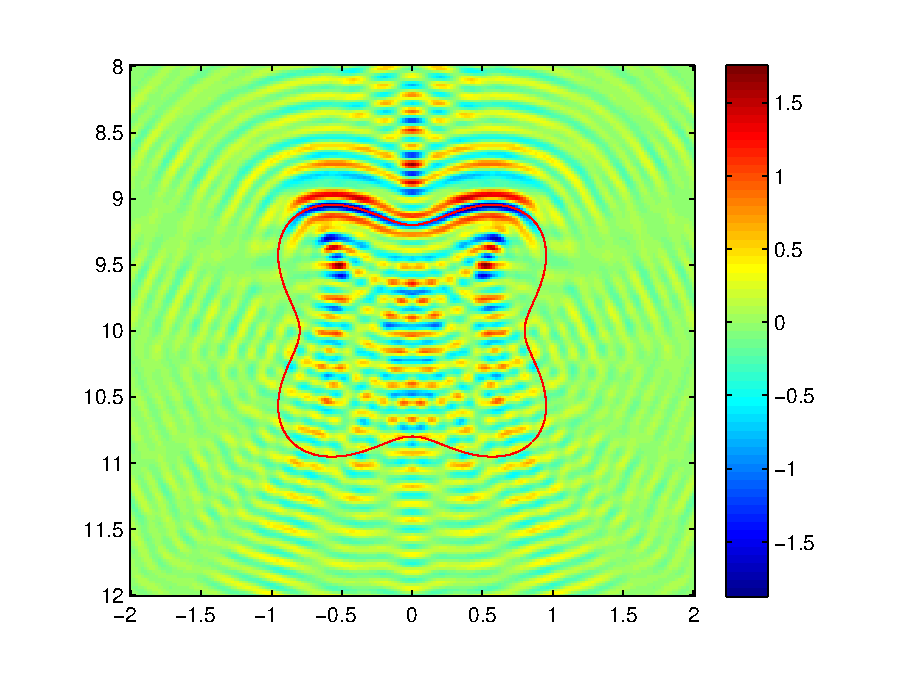
\includegraphics[width=0.24\textwidth]{./graphic/p_leaf_4pi_neumann.eps}
	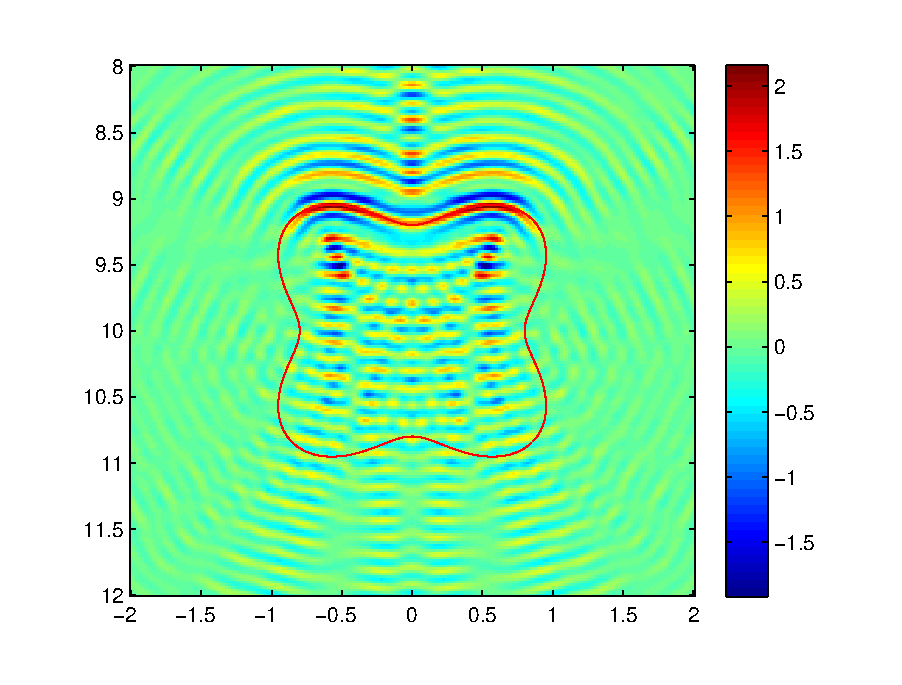
\includegraphics[width=0.24\textwidth]{./graphic/p_leaf_4pi_impedance_1.eps}
	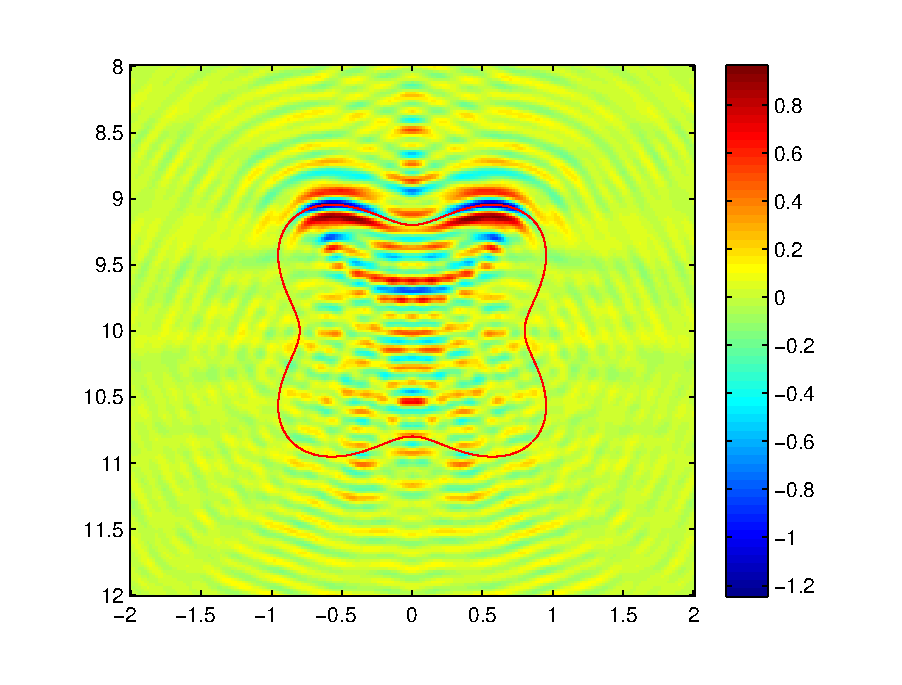
\includegraphics[width=0.24\textwidth]{./graphic/p_leaf_4pi_transmission.eps}
	
	
	\caption{Example 1: From left to right: imaging results of a Neumann, a Robin bounday with impedance $\eta(x)=1$, and a penetrable obstacle with diffractive index $n(x)=0.25$}\label{figure_rtm_half}
\end{figure}
 
\section{Some comment about phaseless imaging, 2018.01.24}

\begin{figure}
	\centering
	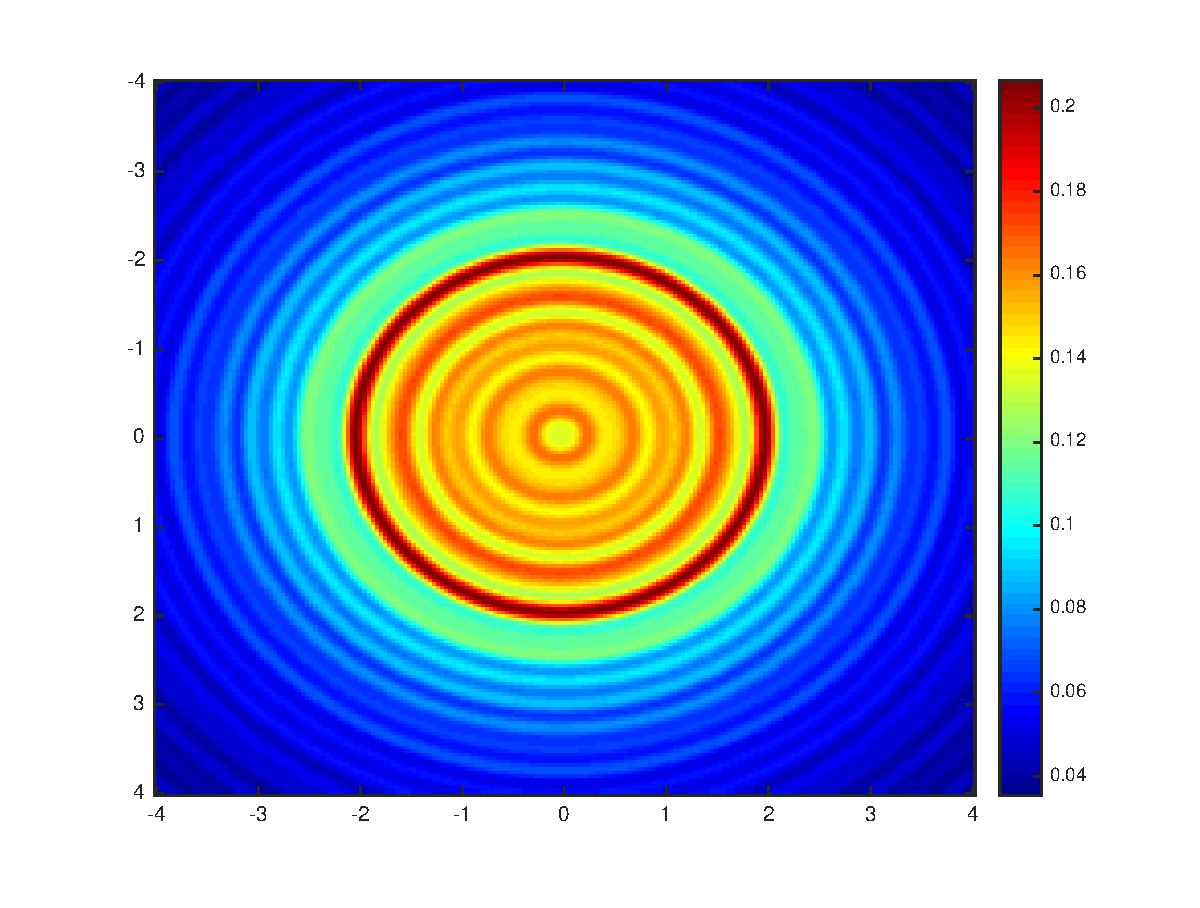
\includegraphics[width=0.24\textwidth]{./graphic_phase/circle_r_10_k_4_vector.eps}
	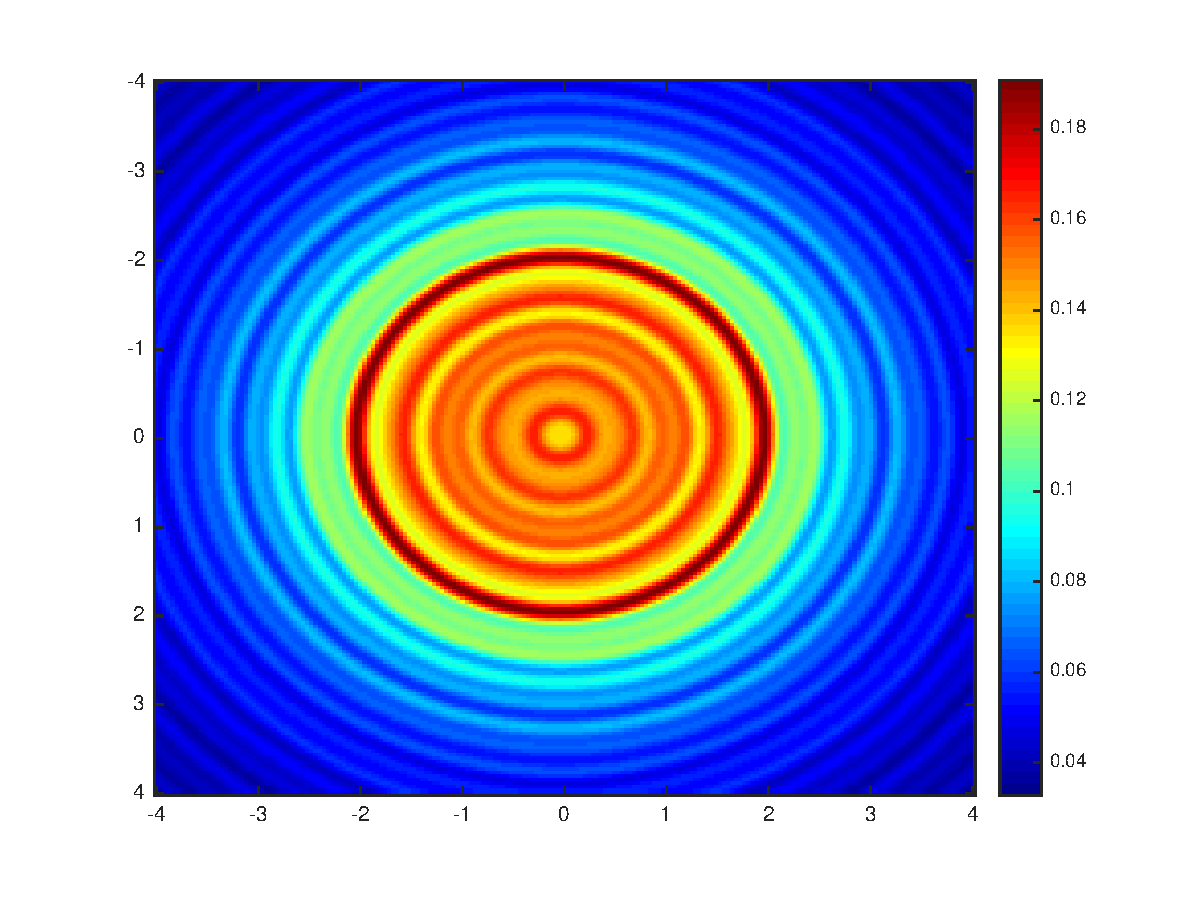
\includegraphics[width=0.24\textwidth]{./graphic_phase/circle_r_10_k_4_scalar.eps}
	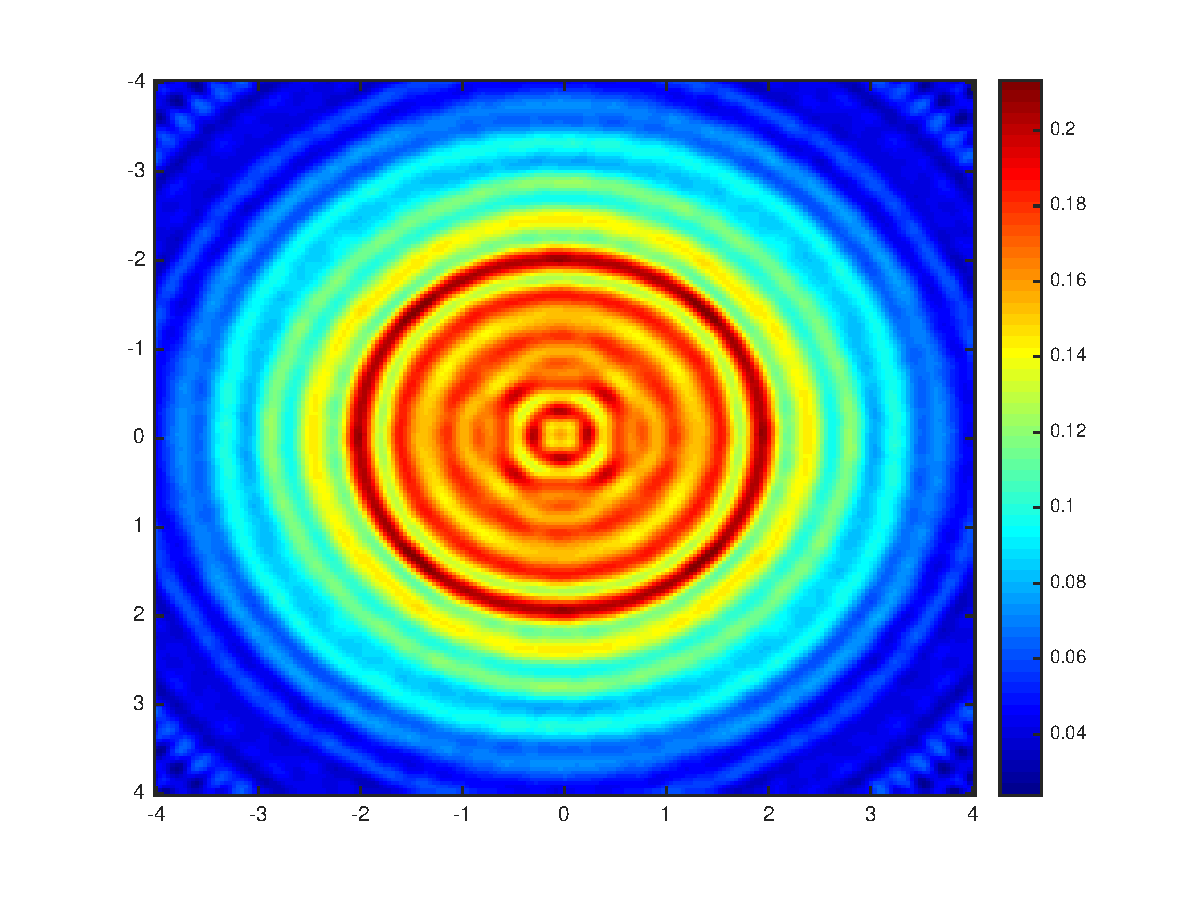
\includegraphics[width=0.24\textwidth]{./graphic_phase/circle_r_10_k_4_phaseless_n_128_bias_100.eps}
	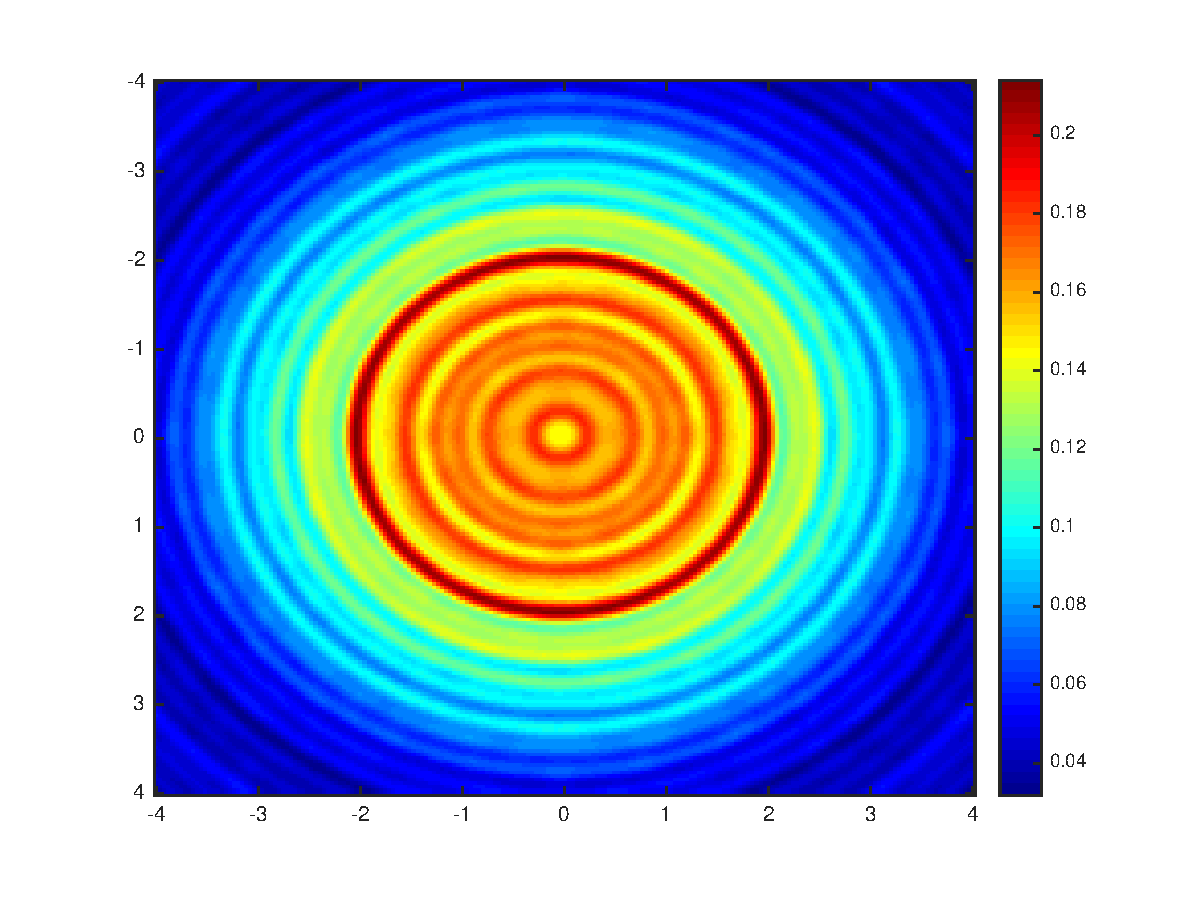
\includegraphics[width=0.24\textwidth]{./graphic_phase/circle_r_10_k_4_phaseless_n_512_bias_100.eps}
	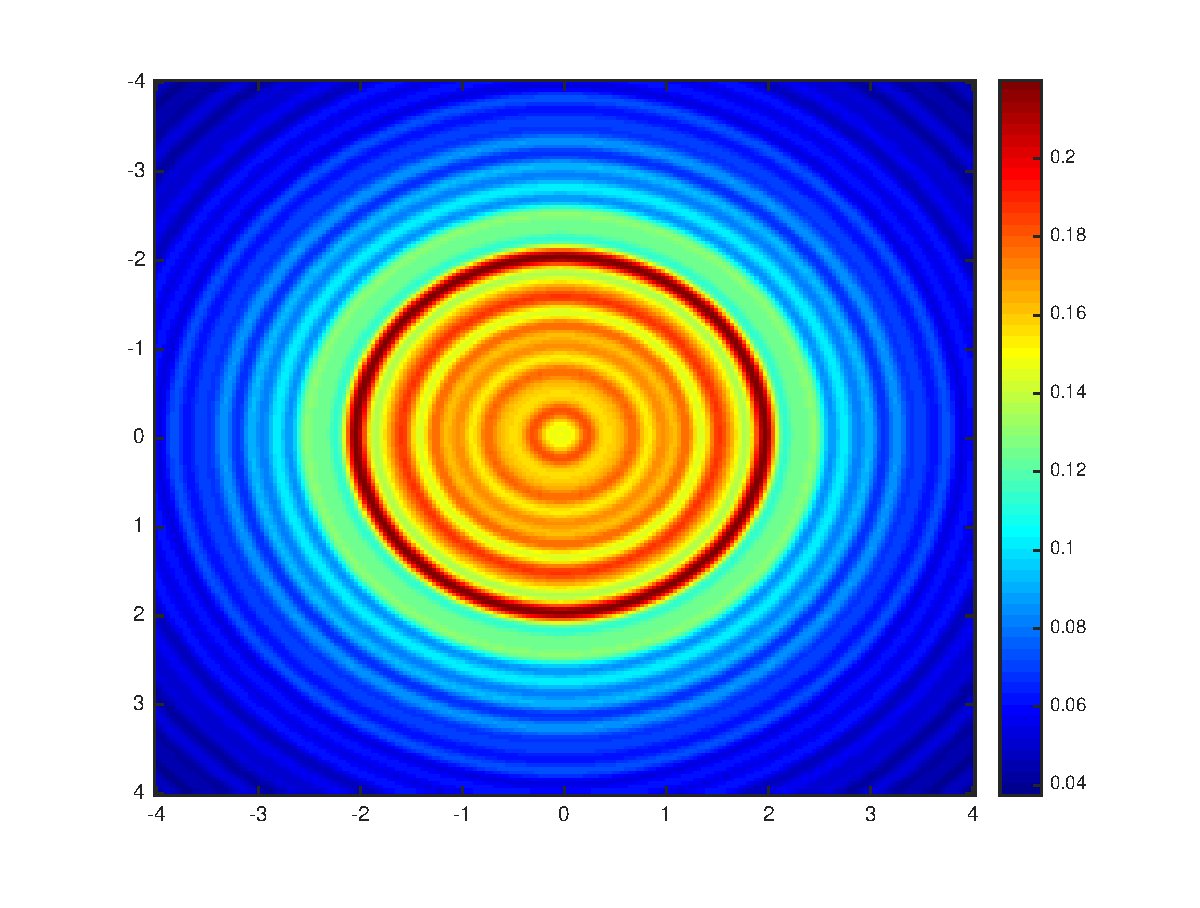
\includegraphics[width=0.24\textwidth]{./graphic_phase/circle_r_100_k_4_vector.eps}
	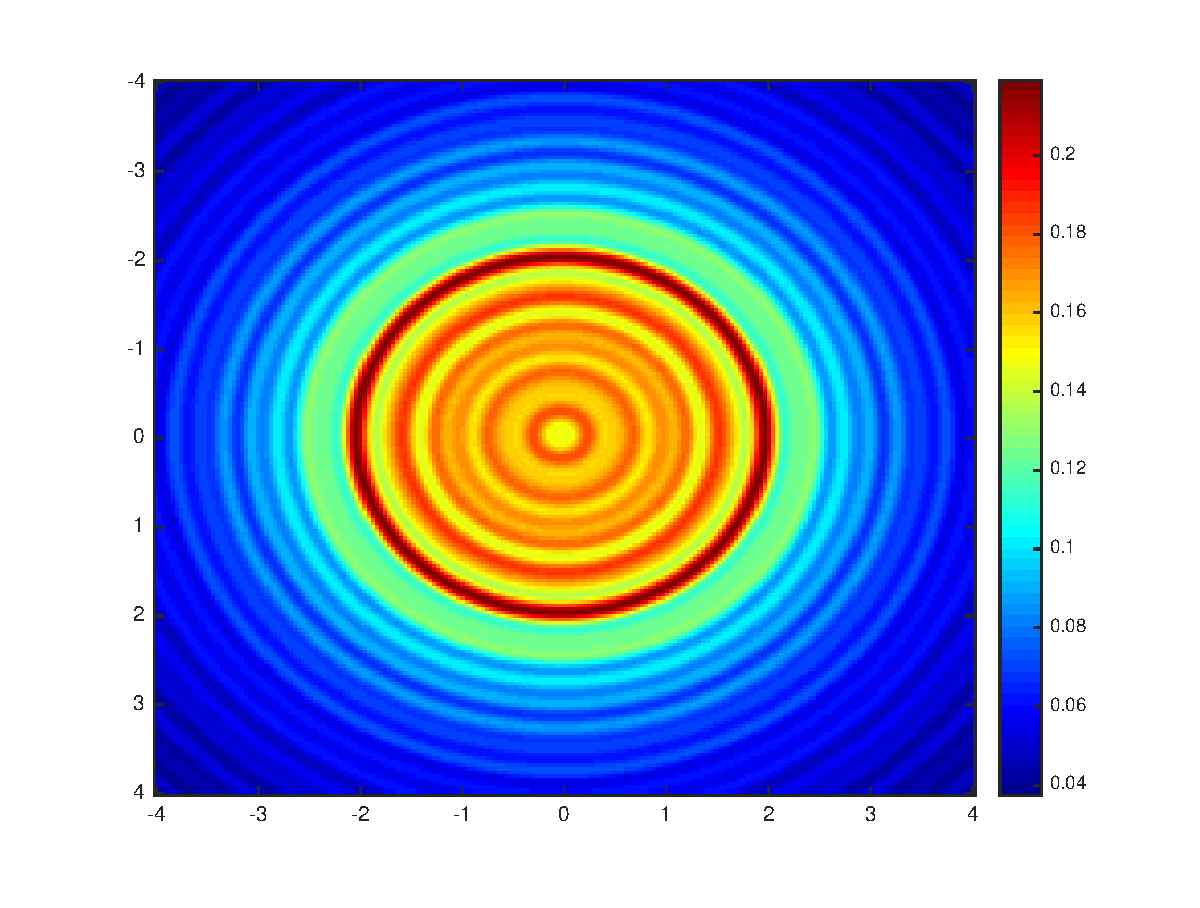
\includegraphics[width=0.24\textwidth]{./graphic_phase/circle_r_100_k_4_scalar.eps}
	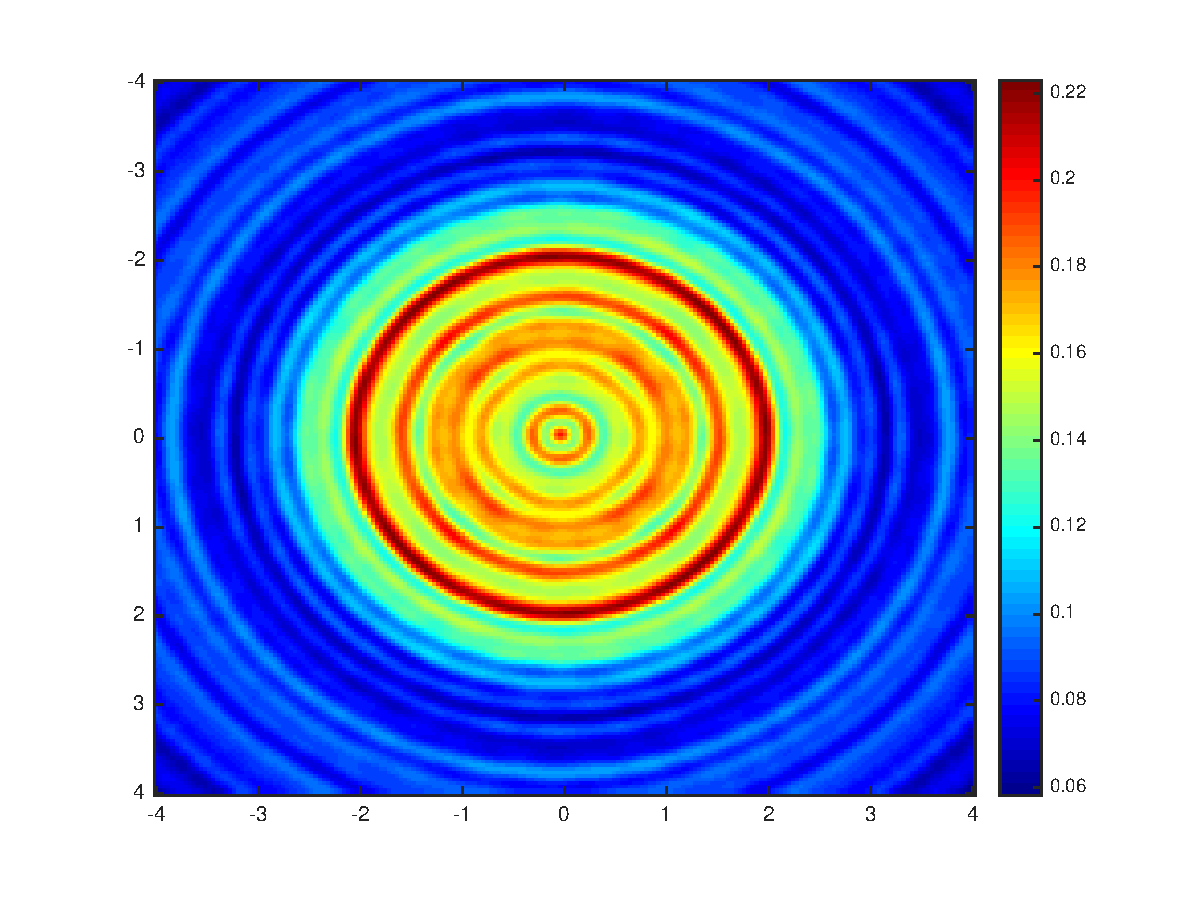
\includegraphics[width=0.24\textwidth]{./graphic_phase/circle_r_100_k_4_phaseless_n_128_bias_100.eps}
	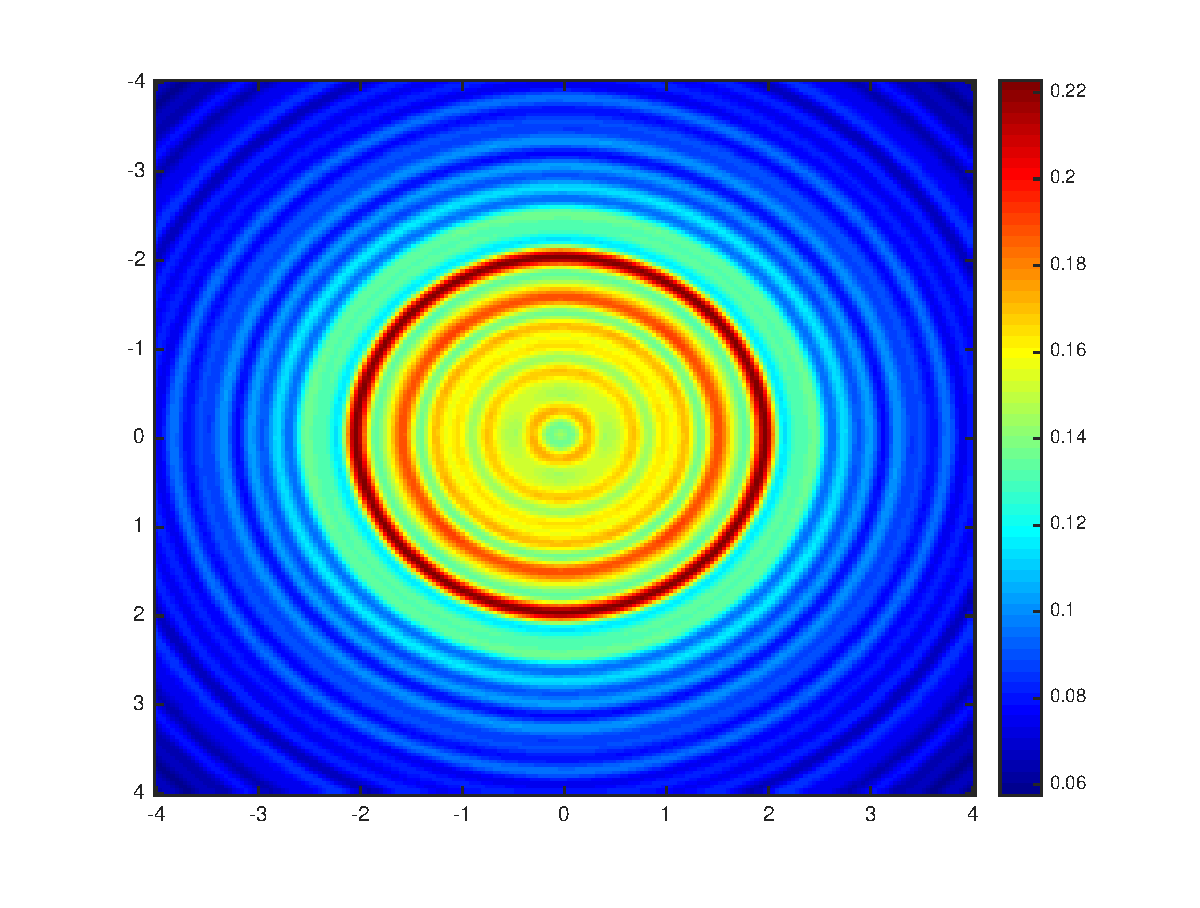
\includegraphics[width=0.24\textwidth]{./graphic_phase/circle_r_100_k_4_phaseless_n_512_bias_100.eps}

	\caption{Circle;From left to right: vector imaging, scalar imaging, phaseless imaging128, phaseless imaging512; From up to down: R=10, R=100 }\label{figure_circle_phaless}
\end{figure}
\begin{figure}
	\centering
	\includegraphics[width=0.24\textwidth]{./graphic_phase/peanut_r_10_k_4_vector.eps}
	\includegraphics[width=0.24\textwidth]{./graphic_phase/peanut_r_10_k_4_scalar.eps}
	\includegraphics[width=0.24\textwidth]{./graphic_phase/peanut_r_10_k_4_phaseless_n_128_bias_100.eps}
	\includegraphics[width=0.24\textwidth]{./graphic_phase/peanut_r_10_k_4_phaseless_n_512_bias_100.eps}
	\caption{Peanut;From left to right: vector imaging, scalar imaging, phaseless imaging128, phaseless imaging512;  }\label{figure_peanut_phaless}
\end{figure}
\begin{figure}
	\centering
	\includegraphics[width=0.24\textwidth]{./graphic_phase/5-leaf_r_10_k_4_vector.eps}
	\includegraphics[width=0.24\textwidth]{./graphic_phase/5-leaf_r_10_k_4_scalar.eps}
	\includegraphics[width=0.24\textwidth]{./graphic_phase/5-leaf_r_10_k_4_phaseless_n_128_bias_100.eps}
	\includegraphics[width=0.24\textwidth]{./graphic_phase/5-leaf_r_10_k_4_phaseless_n_512_bias_100.eps}
	\caption{Peanut;From left to right: vector imaging, scalar imaging, phaseless imaging128, phaseless imaging512;  }\label{figure_5-leaf_phaless}
\end{figure}

\begin{figure}
	\centering
	\includegraphics[width=0.24\textwidth]{./graphic_phase/rectangle_r_10_k_4_vector.eps}
	\includegraphics[width=0.24\textwidth]{./graphic_phase/rectangle_r_10_k_4_scalar.eps}
	\includegraphics[width=0.24\textwidth]{./graphic_phase/rectangle_r_10_k_4_phaseless_n_128_bias_100.eps}
	\includegraphics[width=0.24\textwidth]{./graphic_phase/rectangle_r_10_k_4_phaseless_n_512_bias_100.eps}
	\caption{Peanut;From left to right: vector imaging, scalar imaging, phaseless imaging128, phaseless imaging512;  }\label{figure_rectangle_phaless}
\end{figure}

\begin{figure}
	\centering
	\includegraphics[width=0.24\textwidth]{./graphic_phase/pear_r_10_k_4_vector.eps}
	\includegraphics[width=0.24\textwidth]{./graphic_phase/pear_r_10_k_4_scalar.eps}
	\includegraphics[width=0.24\textwidth]{./graphic_phase/pear_r_10_k_4_phaseless_n_128_bias_100.eps}
	\includegraphics[width=0.24\textwidth]{./graphic_phase/pear_r_10_k_4_phaseless_n_512_bias_100.eps}
	\caption{Peanut;From left to right: vector imaging, scalar imaging, phaseless imaging128, phaseless imaging512;  }\label{figure_pear_phaless}
\end{figure}

\begin{figure}
	\centering
	\includegraphics[width=0.24\textwidth]{./graphic_phase/bi_circle_r_10_k_4_vector.eps}
	\includegraphics[width=0.24\textwidth]{./graphic_phase/bi_circle_r_10_k_4_scalar.eps}
	\includegraphics[width=0.24\textwidth]{./graphic_phase/bi_circle_r_10_k_4_phaseless_n_128_bias_100.eps}
	\includegraphics[width=0.24\textwidth]{./graphic_phase/bi_circle_r_10_k_4_phaseless_n_512_bias_100.eps}
	
	\caption{Circle;From left to right: vector imaging, scalar imaging, phaseless imaging128, phaseless imaging512; From up to down: R=10, R=100 }\label{figure_bicircle_phaless}
\end{figure}

\section{RTM phaseless: elastic; 03.15}
The RTM imaging function studied in \cite{chen2015reverse_elas} for reconstructing extended targets is
\ben
I_1(z)=-\om^2\Im\sum_{q=e_1,e_2}\int_{\Ga_s}\int_{\Ga_r}\bigg(c_pG_p(z,x_rs)q+c_sG_s(z,x_s)q\bigg)\\
\cdot\bigg(c_pG_p(z,x_r)+c_sG_s(z,x_r)\bigg)\overline{u^s_q(x_r,x_s)}ds(x_r)ds(x_s)
\een
For vector $x=(x_1,x_2)^T$, we introduce tow unit vectors $\hat{x}={x}/{|x|}:=(\hat{x}_1,\hat{x}_2)^T$ and $\tilde{x}=(-\hat{x}_2,\hat{x}_1)$. We define $A(x)=\hat{x}\hat{x}^T$ and $B(x)=\tilde{x}\tilde{x}^T$
\ben
I_2(z)=-\om^2\Im\sum_{q=e_1,e_2}\int_{\Ga_s}\int_{\Ga_r}\bigg(k_pg_p(z,x_rs)A(x_s)q+k_sg_s(z,x_s)B(x_s)q\bigg)\\
\cdot\bigg(k_pg_p(z,x_r)A(x_r)+k_sg_s(z,x_r)B(x_r)\bigg)\overline{u^s_q(x_r,x_s)}ds(x_r)ds(x_s)
\een
or
\ben
I_2(z)=-\om^2\Im\sum_{q=e_1,e_2}\int_{\Ga_s}\int_{\Ga_r}\bigg(c_pG_p(z,x_rs)q+c_sG_s(z,x_s)q\bigg)\\
\cdot\bigg(k_pg_p(z,x_r)A(x_r)+k_sg_s(z,x_r)B(x_r)\bigg)\overline{u^s_q(x_r,x_s)}ds(x_r)ds(x_s)
\een
and
\ben
I_3(z)=-\om^2\Im\sum_{q=e_1,e_2}\int_{\Ga_s}\int_{\Ga_r}\bigg(k_pg_p(z,x_rs)A(x_s)q+k_sg_s(z,x_s)B(x_s)q\bigg)\\
\cdot\bigg(k_pg_p(z,x_r)\hat{x_r}D_p(x_r,x_s)+k_sg_s(z,x_r)\tilde{x_r}D_s(x_r,x_s)\bigg)ds(x_r)ds(x_s)
\een
or
\ben
I_3(z)=-\om^2\Im\sum_{q=e_1,e_2}\int_{\Ga_s}\int_{\Ga_r}\bigg(c_pG_p(z,x_rs)q+c_sG_s(z,x_s)q\bigg)\\
\cdot\bigg(k_pg_p(z,x_r)\hat{x_r}D_p(x_r,x_s)+k_sg_s(z,x_r)\tilde{x_r}D_s(x_r,x_s)\bigg)ds(x_r)ds(x_s)
\een
where
\ben
D_p(x_r,x_s)=\frac{|\hat{x_r}^Tu_q(x_r,x_s)|^2-|\hat{x_r}^Tu^i_q(x_r,x_s))|^2}{\hat{x_r}^Tu^i_q(x_r,x_s))} \\
D_s(x_r,x_s)=\frac{|\tilde{x_r}^Tu_q(x_r,x_s)|^2-|\tilde{x_r}^Tu^i_q(x_r,x_s))|^2}{\tilde{x_r}^Tu^i_q(x_r,x_s))}
\een 
Conjecture
\ben
|I_1(z)-I_2(z)|\leq C\frac{1}{k_p R_s}, \ \ |I_2(z)-I_3(z)|\leq C\frac{1}{k_p R_s}
\een
\begin{lem}\label{kir_eq}
	We have
\ben
k_p\int_{|x|=R}g_p(z,x)A(x)\overline{G(x,y)}ds(x)=\Im G_p(z,y) +W_p(y,z)\\
k_s\int_{|x|=R}g_s(z,x)B(x)\overline{G(x,y)}ds(x)=\Im G_s(z,y) +W_s(y,z)
\een
where $|W_\alpha^{ij}(z,y)|+k_\alpha^{-1}|\nabla_z W_\alpha^{ij}(z,y)|\leq C_\alpha R^{-1}$ for some constanc $C_\alpha$ depending on $k_\alpha|z|,k_\alpha|y|$, $\alpha\in\{p,s\}$.
\end{lem}
\debproof
We first recall the following estimate for the first Hankel function in \cite[p.197]{watson1995treatise}, for any $t>0$, we have
\ben\hspace{-2cm}
H^{(1)}_0(t)=\left(\frac 2{\pi t}\right)^{1/2}e^{\i(t-\pi/4)}+R_0(t),\ \ 
H^{(1)}_1(t)=\left(\frac 2{\pi t}\right)^{1/2}e^{\i(t-3\pi/4)}+R_1(t),
\een
where $|R_j(t)|\le Ct^{-3/2}$, $j=0,1$, for some constant $C>0$ independent of $t$. By the defination of Green Tensor, we have
\ben\hspace{-2cm}
G_p(x,y)=\frac{\i}{\sqrt{8\pi}(\lambda+2\mu)}A(x-y)\frac{1}{(k_p|x-y|)^{1/2}}e^{\i k_p|x-y|-\i\frac{\pi}{4}}+O(\frac{1}{(k_p|x-y|)^{3/2}})\\ \hspace{-2cm}
G_s(x,y)=\frac{\i}{\sqrt{8\pi}\mu}B(x-y)\frac{1}{(k_s|x-y|)^{1/2}}e^{\i k_p|x-y|-\i\frac{\pi}{4}}+O(\frac{1}{(k_s|x-y|)^{3/2}})
\een
Some simple manipulation yields:
\ben 
|A(x-y)-A(x)|\leq C_1/|x|, \ \ |B(x-y)-B(x)|\leq C_2/|x| \\
 |\frac{1}{|x-y|}-\frac{1}{|x|}|\leq C_3/|x|^2 , \ \
||x-y|-(|x|-\hat{x}\cdot y)|\leq C_4/|x|
\een
where $C_i$, i=1,2,3,4 depend on $|y|$.
\finproof

Now we turn to the analysisi of the imaging function $I_3(z)$. We first observe that:
\ben
D_p(x_r,x_s)=\hat{x_r}^T\overline{u^s_q}+\frac{|\hat{x_r}^Tu^s_q(x_r,x_s)|^2}{\hat{x_r}^Tu^i_q(x_r,x_s))}+\frac{(\hat{x_r}^Tu^s_q(x_r,x_s))(\hat{x_r}^T\overline{u^i_q(x_r,x_s)})}{\hat{x_r}^Tu^i_q(x_r,x_s))}  \\ 
D_s(x_r,x_s)=\tilde{x_r}^T\overline{u^s_q}+\frac{|\tilde{x_r}^Tu^s_q(x_r,x_s)|^2}{\tilde{x_r}^Tu^i_q(x_r,x_s))}+\frac{(\tilde{x_r}^Tu^s_q(x_r,x_s))(\tilde{x_r}^T\overline{u^i_q(x_r,x_s)})}{\tilde{x_r}^Tu^i_q(x_r,x_s))}
\een

\section{Estimate by hankel methon,03.30}
Preminary:
\ben
\cos\theta=1-2\sin^2\frac{\theta}{2}:=1-t^2\\
t=e^{-\i\frac{\pi}{4}}s\\
\sin\theta(s):=S(s)=e^{-\i\frac{\pi}{4}}s(2+\i s^2)^{-1/2}\cos\phi+(1+\i s^2)\sin\phi \\
\cos\theta(s):=C(s)=(1+\i s^2)\cos\phi-e^{-\i\frac{\pi}{4}}s(2+\i s^2)^{-1/2}\sin\phi \\
\cos\frac{\theta(s)}{2}=(2-(t(s))^2)^{1/2}=(2+\i s^2)^{1/2}
\een
\section{04.02}
Let $f(\xi):=h(\xi,\mu(\xi),\mu_\kappa(\xi))$ be a analytic function with respect to $\xi$ in $\C\bks\{\i\R\cup(-1,1)\}$. For any $a,b>0$, we denote
\ben
I(f;a,b)=\int_{\R}f(\xi)e^{\i a\xi+\i b\mu(\xi)}d\xi
\een
where $\mu(\xi)=(1-\xi^2)^{1/2}$, $\mu_\kappa(\xi)=(\kappa-\xi^2)^{1/2}$.
\begin{lem}\label{new_station_phase}
	Let $a,b >0$, $\rho=\sqrt{a^2+b^2}$, and $f(\xi):=h(\xi,\mu(\xi),\mu_\kappa(\xi))$ be a analytic function in $\C\bks\{\i\R\cup(-1,1)\}$. Then 
	\ben\hspace{-2.5cm}
	I(f;a,b)=\sqrt{\frac{2}{\rho}}e^{\i\rho-\i\pi/4}\int_{\R}F(\frac{t}{\sqrt{\rho}})C(\frac{t}{\sqrt{\rho}})e^{-t^2}dt+
	O(\rho^{-3/2})\|F(\frac{t}{\sqrt{\rho}})C(\frac{t}{\sqrt{\rho}})t^2e^{-t^2}\|_{L^1(\R)}
	\een
	where $F(s)= h(S(s),C(s),\mu_\kappa(S(s))$ and $\sin\phi=a/\rho,\cos\phi=b/\rho$.
\end{lem}
\debproof
 To simplify the integral, the standard substitution $\xi=k_s\sin \theta$ is made, taking the $\xi$-plane to a strip $-\pi/2<\Re \theta <\pi/2$ in the $\theta$-plane, and the real axis in the $\xi$-plane onto the path L from $-\pi/2+\i\infty\rightarrow-\pi/2\rightarrow\pi/2\rightarrow\pi/2-\i\infty$ in the $\theta-plane$. The integral $I(f;a,b)$ then becomes( Let a=$\rho \sin\phi$  and b=$\rho\cos\phi$, $0<\phi<\pi/2$)
\be
 I(f;a,b)=\int_L h(\sin \theta,\cos \theta,\mu_\kappa(\sin \theta))\cos \theta \ e^{\i\rho(\cos (\theta-\phi))} d\theta
\ee
Taking the shift transformation of $\theta$ and using cauchy integral theorem, we can obtain the more useful representation of $I(f;a,b)$:
\be
I(f;a,b)=\int_L f(\sin (\theta+\phi))\cos (\theta+\phi) \ e^{\i\rho\cos \theta} d\theta
\ee
\begin{figure}
	\centering
	\includegraphics[width=0.4\textwidth]{./graphic/transform_th.png}
	\includegraphics[width=0.4\textwidth]{./graphic/transform_t.png}

	\caption{integral path in $\theta-plane$ and t-plane  }\label{transform_t}
\end{figure}
Notice that $\cos\theta=1-2\sin^2\frac{\theta}{2}$, by substituting $\theta(t)=2\arctan\frac{\sqrt{2}t}{2}$, we get:
\ben\hspace{-1.5cm}
I(f;a,b)=e^{\i\rho}\int_{L_1\cup(-1,1)\cup L_2} f(\sin (\theta(t)+\phi))\cos (\theta(t)+\phi)\frac{2}{(2-t^2)^{1/2}} \ e^{-\i\rho t^2} dt
\een
where 
\ben
L1=\{t|(\Re t)^2-(\Im t)^2=1,\Re t <0,\Im t>0\}\\
L2=\{t|(\Re t)^2-(\Im t)^2=1,\Re t >0,\Im t<0\}
\een
and the geometry is depicted in Figure \ref{transform_t}. A simple computation show that the substitution $\theta(t)=2\arctan\frac{\sqrt{2}t}{2}$ transform the domain $\Omega_\theta=\{\theta||\Re\theta|<\pi, \Re\theta\cdot\Im\theta<0\}$ in the $\theta$-plane into $\Omega_t=\{t| \Re t\cdot\Im t<0\}$ in t-plane. Now it is easy to see that $f(\sin(\theta(t)_\phi))$ is analytic in the domain $\Omega_t$. Since $\Omega_t$ is surrounded by $L_1\cup L_2\cup(-1,1)$ and the diagonal line of the second and the fourth quadrants denote by $L3$, by using Cauchy integral theorem, we have
\ben\hspace{-1.5cm}
I(f;a,b)=e^{\i\rho}\int_{L_3} f(\sin (\theta(t)+\phi))\cos (\theta(t)+\phi)\frac{2\cos (\theta(t)+\phi)}{(2-t^2)^{1/2}} \ e^{-\i\rho t^2} dt \\ \hspace{-1.5cm}
=e^{\i\rho-\i \pi/4}\int_{\R} f(\sin (\theta(e^{-\i\pi/4 s})+\phi))\frac{2\cos (\theta(e^{-\i\pi/4 s})+\phi)}{(2+\i s^2)^{1/2}} \ e^{-\rho s^2} ds \\
 \hspace{-1.5cm}
=e^{\i\rho-\i \pi/4}\int_{\R} f(S(s))\frac{2C(s)}{(2+\i s^2)^{1/2}} \ e^{-\rho s^2} ds \\
\hspace{-1.5cm}
=\sqrt{\frac{2}{\rho}}e^{\i\rho-\i \pi/4}\int_{\R} f(S(\frac{t}{\sqrt{\rho}}))C(\frac{t}{\sqrt{\rho}}){(1+\i \frac{t^2}{2\rho})^{-1/2}} \ e^{-t^2} dt
\een
The lemma follows immediately from the fact that $(1+\i s)^{-1/2}=1+O(|s|),s\in\R$. The proof is completed.
\finproof
The following lemma is a directed consequence of lemma \ref{new_station_phase}
\begin{lem}
	Let p(x,y,z) be a homogeneous polynomial of degree 2 and $f(\xi)=p(\xi,\mu(\xi),\mu_\kappa(\xi))/(\xi^2+\mu(\xi)\mu_\kappa(\xi))$. Then for $\rho>1$, we have
	\ben
	|I(f;a,b)|\leq C(\frac{b}{\rho}\rho^{-1/2}+\frac{a}{\rho}\rho^{-5/4}+\rho^{-3/2})
	\een
	where C is a constant independant of $a,b$.
\end{lem}
\debproof
By lemme \ref{new_station_phase}, it suffices to estimate the integral $I(\rho)$ where
\ben
I(\rho)=\int_{\R}F(\frac{t}{\sqrt{\rho}})C(\frac{t}{\sqrt{\rho}})e^{-t^2}dt \\
= \cos\phi\int_{\R}F(\frac{t}{\sqrt{\rho}})(1+\i\frac{t^2}{\rho})e^{-t^2}dt-\frac{1}{\rho}\sin\phi\int_{\R}e^{-\i\pi/4} F(\frac{t}{\sqrt{\rho}})(2+\i\frac{t^2}{\rho})^{1/2}te^{-t^2}dt \\
:=\frac{b}{\rho}\phi I_1(\rho)-\frac{1}{\rho}\frac{a}{\rho} e^{-\i\pi/4} I_2(\rho)
\een
For $s\in\R$, it is easy to check that
\ben
\max\{|S(s)|,|C(s)|\}\leq |s(2+\i s^2)^{1/2}|+|1+\i s^2|\leq C(1+s+s^2)\\
|\mu_\kappa(C(s))|\leq C(1+|S(s)|)\leq C (1+s+s^2) 
\een
where C is independent of $\phi$. Consequently, for $\rho>1$, we obtain
\ben
|I_1(\rho)|\leq\int_\R |p(S(\frac{t}{\sqrt{\rho}}),(\frac{t}{\sqrt{\rho}}),\mu_\kappa(S(\frac{t}{\sqrt{\rho}})))|(1+\frac{t^2}{\rho})e^{-t^2}dt \\
\leq C\int_\R\sum_{k=0}^{6}\frac{t}{\sqrt{\rho}}e^{-t^2}dt\leq C
\een
Before estimating $I_2(\rho)$, we need to deal with term $\mu_\kappa(S(s))$. Let $\kappa=\sin_\kappa,0<\theta_\kappa<\pi/2$, then we have
\ben
|\mu_\kappa(S(s))|^2=|\sin^2\theta(s)-\sin^2(\theta(s)+\phi)|\\
=4|\sin\frac{\theta(s)+\theta_\kappa+\phi}{2}||\cos\frac{\theta(s)+\theta_\kappa+\phi}{2}||\cos\frac{\theta(s)-\theta_\kappa+\phi}{2}||\sin\frac{\theta(s)-\theta_\kappa+\phi}{2}| \\
\geq C|\sin\frac{\theta(s)-\theta_\kappa+\phi}{2}| \\
\geq C(|s\cos\frac{\theta_\kappa-\phi}{2}+\sqrt{\sqrt{4+s^2}+2}\sin\frac{\theta_\kappa-\phi}{2}|+|s\cos\frac{\theta_\kappa-\phi}{2}-\sqrt{\sqrt{4+s^2}-2}\sin\frac{\theta_\kappa-\phi}{2}|) \\
\geq C s
\een
Now using integration by parts and inequality above, we get
\ben
|I_2(\rho)|\leq\frac{1}{\sqrt{\rho}}\int_\R\Big( |F'(\frac{t}{\sqrt{\rho}})||2+\frac{t^2}{\rho}|^{1/2}+|F(\frac{t}{\sqrt{\rho}})|\Big)e^{-t^2}dt \\
\leq C\frac{1}{\sqrt{\rho}}\int_\R |F'(\frac{t}{\sqrt{\rho}})|e^{-t^2}dt + C\frac{1}{\sqrt{\rho}} \\
\leq C\frac{1}{\sqrt{\rho}}\int_\R |\mu_\kappa(S(\frac{t}{\sqrt{\rho}}))|^{-1}e^{-t^2}dt + C\frac{1}{\sqrt{\rho}}\\
\leq C \frac{1}{\rho^{1/4}}
\een
By the smae procedure as above, it is easy to see that
\ben
\|F(\frac{t}{\sqrt{\rho}})C(\frac{t}{\sqrt{\rho}})t^2e^{-t^2}\|_{L^1(\R)}\leq C
\een
This completes the proof.
\finproof
\section*{References}
\bibliography{eee}
\end{document}
